%TODO : Mein eigenes Verwendetes System beschreiben, genauer, welche verschiedenen Interaktionen hatte ich, etc. Warum habe ich was gemacht, eventuell sogar mit UML Diagrammen arbeiten
%
%Auch weitere Hypoethesen in Sachen präsenz als zusätzliches Kapitel "Signifikanzanalyse" oder so mit hineinbringen. Nur die, die Signifikant sind.
%
%Analyse mit Signifikanzniveau von 10% anschauen, damit Ergebnisse schnelller Signifikant sind.
%
%Umbenennung von "VR" und "AVATARE" etc.
%
%Nicht alles so kleingliedrig
%
%Auf Verwendung von nicht parametrische Tests achten.
%
%Leseprobe senden!
%Auswertungen nicht als Screenshot sondern als Tabelle
%Gerichtete Hypothese überprüfen, schauen ob der p-Wert halbiert werden kann
\documentclass[a4paper,11pt]{article}%Schriftgröße

\usepackage{booktabs}
\usepackage{multirow}
\usepackage{rotating}
\newcommand\tabrotate[1]{\begin{turn}{90}\rlap{#1}\end{turn}}
\usepackage{varwidth}
\newcommand\tabvarwidth[2][3cm]{\begin{varwidth}[b]{#1}\centering #2\end{varwidth}}
\usepackage{tabularx}
\usepackage{amsmath}

\usepackage[T1]{fontenc} 
\usepackage[utf8]{inputenc}
\usepackage[ngerman]{babel}%Veröffentlichungssprache
\usepackage{graphicx}
\usepackage{ragged2e}
\usepackage[format=plain,justification=RaggedRight,singlelinecheck=false,font={small},labelsep=space]{caption}
\usepackage{float}
\usepackage{xcolor}	
\usepackage[a4paper]{geometry}
\usepackage{fancyhdr}
\usepackage[onehalfspacing]{setspace}%Zeilenabstand
\usepackage[onehalfspacing]{setspace}%Zeilenabstand
\usepackage{fancyhdr}
\usepackage[authoryear]{natbib}
\usepackage{relsize}
\usepackage[printonlyused, smaller, footnote]{acronym}
%\usepackage[printonlyused, withpage, smaller, footnote]{acronym}
\renewcommand{\\}{\vspace*{0.5\baselineskip} \newline}
\renewcommand*\MakeUppercase[1]{#1}	
\renewcommand{\familydefault}{\sfdefault}
\geometry{left=3.5cm,right=2.5cm,top=2.4cm,bottom=2cm}%Seitenränder
\pagestyle{fancy}
\renewcommand{\headrulewidth}{0pt}
\renewcommand{\footrulewidth}{0pt}
\fancyhead[R]{\footnotesize{\thepage}}
\fancyhead[L]{\footnotesize{\leftmark}}
\fancyfoot{}
\usepackage[colorlinks,pdfpagelabels,pdfstartview = FitH,bookmarksopen = true,bookmarksnumbered = true,linkcolor = black,urlcolor = black,plainpages = false,hypertexnames = false,citecolor = black] {hyperref}

\begin{document}
	\begin{titlepage}
		\begin{flushleft}
			\vspace*{-1cm}
			
\includegraphics[scale=1]{Abbildungen/TH.png}\\
			\vspace*{1cm}
		\end{flushleft}
		
		\begin{huge}
			\noindent
			%Vergleich des Teambuildingerfolgs mittels eines nicht-vollkörpergetracktem- und vollkörpergetracktem Avatars in einer Immersive Virtual Reality anhand einer Escape-Room-Artigen Umgebung. \\
			
%			Vertrauensaufbau einer Teambuildingmaßnahme zwischen eines Hand- und Kopf getracktem Avatar und  eines Hand-, Kopf und Inverskinematisch-simuliertem Torsos getracktem Avatar in einem Shared Virtual Environment anhand einer Escape-Room-Artigen Umgebung. \\
			
%			Auswirkung des Vertrauens auf die Effizienz in einer Teambuildingmaßnahme anhand eines Hand- und Kopfgetracktem und einem Hand-, Kopf und Inverskinematisch-simuliertem Torsos getracktem Avatar ein einem Shared Virtual Environment. //
			
%			Auswirkung von Vertrauen zu Avataren auf die \mbox{Effizienz} in einer Teambuildingmaßnahme in ein einem Shared Virtual Environment.

%Auswirkung des Vertrauens einer Teambuildingmaßnahme anhand eines \dq{}IK-Avatar\dq{}und einem \dq{}Non-IK-Avatar\dq{} in einem Shared-Virtual-Environment. \\
%
%Auswirkung des Vertrauens auf die Effizienz einer Teambuildingmaßnahme anhand eines \dq{}IK-Avatar\dq{}und einem \dq{}Non-IK-Avatar\dq{} in einem Shared-Virtual-Environment. \\
%
%Welche Avatarkondition schafft in meinem Team mehr Vertrauen? Hat dieses geschaffene Vertrauen eine Auswirkung auf die Effizienz meiner Teambuildingmaßnahme? Welche Avatarkondition sollte ich also nutzen, um Vertrauen zu schaffen, sodass in einem Team ein effizienteres Arbeiten stattfinden kann?

%Auswirkung von Vertrauen auf die Anfangsphase einer virtuellen Teamgrün

Einfluss der Vertrauensbildung zwischen \ac{ik} und \ac{nik} Avataren auf die Team-Effektivität in einem kurzzeitig zusammenarbeitendem virtuellem Team.\\
		\end{huge}
		
		Masterarbeit zur Erlangung des Master-Grades \newline
		\textit{Master of Science} im Studiengang Medientechnologie \newline
		an der Fakultät für Informations-, Medien- und Elektrotechnik \newline
		der Technischen Hochschule Köln \\
		~\\
		~\\
		~\\
		\noindent\begin{tabular}{ll}
			vorgelegt von: & Hannes Hinrichs \\
			Matrikel-Nr.: &	11121733 \\
			Adresse: & Zülpicher Straße 19 \\
			~ &	50674 Köln \\
			~ &	hannes.hinrichs@web.de \\
			~ & ~ \\
			eingereicht bei: & Prof. Dr. Arnulph Fuhrmann \\
			Zweitgutachter/in: & Prof. Dr. Stefan Grünvogel
		\end{tabular}	
		~\\
		~\\
		Ort, TT.MM.JJJJ
	\end{titlepage}
	\pagenumbering{Roman}
	\pagestyle{fancy}
	\newpage
\section*{Erklärung}\markboth{Erklärung}{Erklärung}\addcontentsline{toc}{section}{Erklärung}
	Ich versichere, die von mir vorgelegte Arbeit selbstständig verfasst zu haben. Alle Stellen, die wörtlich oder sinngemäß aus veröffentlichten oder nicht veröffentlichten Arbeiten anderer oder der Verfasserin/des Verfassers selbst entnommen sind, habe ich als entnommen kenntlich gemacht. Sämtliche Quellen und Hilfsmittel, die ich für die Arbeit benutzt habe, sind angegeben. Die Arbeit hat mit gleichem Inhalt bzw. in wesentlichen Teilen noch keiner anderen Prüfungsbehörde vorgelegen.\\
	Anmerkung: In einigen Studiengängen steht die Erklärung am Ende des Textes.\\
	~\\
	~\\
	\rule{0.35\textwidth}{0.4pt} \hspace*{3cm} \rule{0.45\textwidth}{0.4pt} \newline
	Ort, Datum	\hspace*{6.3cm}	Rechtsverbindliche Unterschrift
	\newpage
\section*{Kurzfassung/Abstract}\markboth{Kurzfassung/Abstract}{Kurzfassung/Abstract}\addcontentsline{toc}{section}{Kurzfassung/Abstract}
	Virtual Reality \ac{vr} hat in den letzten Jahren aufgrund von verbesserter Technologie und sinkenden Kosten an Bedeutung gewonnen. Verschiedene Felder, wie Medizin, Wirtschaft, Training oder die Industrie greifen auf diese Technologie zurück. Voranschreitende Forschung in diesem Feld, ist aufgrund von wachsendem Interesse von großer Bedeutung. Vertrauensbildung und das gesamte Konstrukt von Vertrauen ist in vielen Feldern eine wichtige Grundlage, wurde in der Forschung im Zusammenhang mit \ac{vr} jedoch in den letzten Jahren wenig betrieben. Diese Arbeit zielt darauf ab, das Konstrukt des Vertrauens in der Virtuellen Welt besser zu verstehen und mit diesem umzugehen. Dafür wurde eine Studie der Technischen Hochschule zu Köln durchgeführt, um einen Zusammenhang der Vertrauensbildung in einer Teambuildingmaßnahme zwischen einem Menschenähnlichen Avatar und einem nicht-Menschenähnlichen Avatar, darzustellen.
	
			\paragraph{Virtual-Reality, Vertrauen, Teambuilding, Avatar}
	\newpage
	\tableofcontents
	\newpage
	
\section*{Abkürzungsverzeichnis}\markboth{Abkürzungsverzeichnis}{Abkürzungsverzeichnis}\addcontentsline{toc}{section}{Abkürzungsverzeichnis}
	\begin{acronym}[NIK-T.Lvl.Rounds]
	\acro{hmd}[HMD]{Head-Mounted-Display}
	\acro{sve}[SVE]{Shared-Virtual-Environment}
	\acro{vr}[VR]{Virtual-Reality}
	\acro{ivr}[IVR]{Immersive-Virtual-Reality}
	\acro{ipo}[IPO]{Input-Process-Output}
	\acro{fov}[FOV]{Field-of-View}
	\acro{bip}[BIP]{Break-in-Presence}
	
	\acro{ik}[IK]{Invers-Kinematisch - (Hand-, Kopf und Inverskinematisch-simulierter Torso)}
	\acro{nik}[NIK]{Nicht-Invers-Kinematisch (Hand- und Kopf getrackter Avatar)}
	
	\acro{gt}[GT]{Generelles Vertrauen}
	\acro{gti}[GTI]{Generelles Vertrauen - IK}
	\acro{gtn}[GTN]{Generelles Vertrauen - NIK}
	
	\acro{ct}[CT]{Kognitives Vertrauen}
	\acro{cti}[CTI]{Kognitives Vertrauen - IK}
	\acro{ctn}[CTN]{Kognitives Vertrauen - NIK}
	
	\acro{tc}[TC]{Team-Kommunikation}
	\acro{tci}[TCI]{Team-Kommunikation - IK}
	\acro{tcn}[TCN]{Team-Kommunikation - NIK}
	
	\acro{tRound}[T.Lvl.Rounds]{Erfolgreich abgeschlossene Runden auf Team-Level}
	\acro{tRoundIK}[IK-T.Lvl.Rounds]{Erfolgreiche abgeschlossene Runden auf Team-Level - IK}
	\acro{tRoundNIK}[NIK-T.Lvl.Rounds]{Erfolgreiche abgeschlossene Runden auf Team-Level - NIK}
	
	\acro{te}[TE]{Teameffektivität}
	\acro{tei}[TEI]{Teameffektivität - IK}
	\acro{ten}[TEN]{Teameffektivität - NIK}
	
	\acro{cp}[CP]{Co-Präsenz}
	\acro{cpi}[CPI]{Co-Präsenz - IK}
	\acro{cpn}[CPN]{Co-Präsenz - NIK}
	
	\acro{tlx}[NTLX]{Nasa-TLX}
	\acro{tlxi}[NTLXI]{Nasa-TLX - IK}
	\acro{tlxn}[NTLXN]{Nasa-TLX - NIK}
	
	\acro{teamCog}[T.Lvl.Cog]{Kognitives Vertrauen auf Team-Level}
	\acro{teamCogIK}[IK-T.Lvl.Cog]{Kognitives Vertrauen auf Team-Level - IK}
	\acro{teamCogNIK}[NIK-T.Lvl.Cog]{Kognitives Vertrauen auf Team-Level - NIK}
	
	\acro{teamGen}[T.Lvl.Gen]{Generelles Vertrauen auf Team-Level}
	\acro{teamGenIK}[IK-T.Lvl.Gen]{Generelles Vertrauen auf Team-Level - IK}
	\acro{teamGenNIK}[NIK-T.Lvl.Gen]{Generelles Vertrauen auf Team-Level - NIK}
	
	\acro{scp}[SCP]{Self-Co-Präsenz}
	\acro{scpi}[SCPI]{Self-Co-Präsenz - IK}
	\acro{scpn}[SCPN]{Self-Co-Präsenz - NIK}	
	
	\acro{ocp}[OCP]{Other-Co-Präsenz}
	\acro{ocpi}[OCPI]{Other-Co-Präsenz - IK}
	\acro{ocpn}[OCPN]{Other-Co-Präsenz - NIK}	
	
	\acro{ipq}[IPQ]{Fragebogen des Anstrengungsmaß}
	\acro{ipqi}[IPQI]{Fragebogen des Anstrengungsmaß - IK}
	\acro{ipqn}[IPQN]{Fragebogen des Anstrengungsmaß - NIK}
	
	\acro{tp}[TP]{Telepresence}
	\acro{tpi}[TPI]{Telepresence - IK}
	\acro{tpn}[TPN]{Telepresence - NIK}	
	
	\acro{sp}[SP]{Social-Presence}
	\acro{spi}[SPI]{Social-Presence - IK}
	\acro{spn}[SPN]{Social-Presence - NIK}
	
	\acro{vts}[VT's]{Virtuelle Teams}
%	iktc teamCogIK
%	niktc teamCogNIK
%	tCog teamCog
\end{acronym}

	
	%\newpage
	%\listoftables\addcontentsline{toc}{section}{Tabellenverzeichnis}
	%\newpage
	%\listoffigures\addcontentsline{toc}{section}{Abbildungsverzeichnis}
	\newpage
	\pagenumbering{arabic}
	
%\section{Abgrenzung zu anderen Studien}
%	\begin{itemize}
%	\item{Team besteht aus 3! Personen}
%	\item{Es wird die initiale Anfangsphase eines Teams untersucht}
%	
%	\item{Es wird geschaut, ob das geschaffene Vertrauen eine Auswirkung auf die Team-Effizienz hat}
%	\item{Es wird schaut, mit welcher Kondition ( Self-Avatar vs. non Self-Avatar ) mehr Vertrauen in das Team geschaffen wurde}
%	\item{Es wird geschaut, mit welcher Kondition ( Self-Avatar vs non Self-Avatar ) eine höhere Team-Effizienz wird}
%	\end{itemize}		
	
	
\section*{Einleitung}\markboth{Einleitung}{Einleitung}\addcontentsline{toc}{section}{Einleitung}
	Mit voranschreitender technologischer Entwicklung, rückt die digitale Kommunikation immer mehr in den Mittelpunkt. Unternehmen weltweit setzen schon seit langem darauf, räumliche und zeitliche Grenzen zu überwinden. Begonnen mit der Implementierung eines Telegrafennetz in den 1840er Jahren über das Telefon in den 1870er Jahren bis hin zur E-Mail 1970 und dem World-Wide-Web einige Jahre später.
	Seit den 1990er Jahren ist die Kommunikation mittels Computer nicht mehr wegzudenken. Der Computer steht in jedem Büro, in nahezu jedem Haushalt. Chats, E-Mails, das World-Wide-Web sowie Video- und Sprachkommunikation sind zu Standartkommikationsmittel der heutigen Zeit geworden. \citep[p. 14-16]{thurlow2004computer} \\ 
Neue Generationen von Sozialen-Netzwerksystemen werden mit der Prämisse erstellt, die Kommunikation zu entfernten Personen zu verbessern.
Einsatzfelder sind dabei :
\begin{itemize}
	\item{\textbf{Gemeinsame Arbeitsumgebungen}: Gemeinsame Arbeitsumgebungen sind zunehmend auf digitale Kommunikation angewiesen.}
	\item{\textbf{Die Mobil- und Internettelefonie:} Die Mobil- und Internettelefonie bieten zunehmend ständigen, von Raum und Zeit unabhängigen, sozialen Kontakt zu anderen Nutzern}
	\item{\textbf{Agentenbasierte Hilfsschnitstellen:} Hilfsagenten auf Websites, Charaktere in \ac{sve}'s sowie Charaktere in Computerspielen bieten \dq{}quasi\dq{}-sozialbeziehungen. Diese \dq{}quasi\dq{}-sozialen Beziehungen bieten eine neue Formen von Mensch-Maschinen-Kommunikation in \ac{sve}'s.} 
	\item{\textbf{FOIP/VOIP-Telefonkonferenzen:} Telekonferenzen ermöglichen eine simulierte Kommunikation von Angesicht zu Angesicht und weitere Soziale-Interaktionmöglichkeiten.}
	\item{\textbf{Sprach-interfaces:} Simulationen von sozialen Interaktionen mit dem Computer durch die menschlichen Sprache.}
	\item{\textbf{Soziale virtuelle 3D-Umgebungen:} Ermöglichen eine soziale Interaktion mit vollständig dargestellten Avataren.}
\end{itemize}

All diese Technologien teilen das selbe Ziel : \\ \dq{}Die Verbesserung der Social-Presence, so dass der Nutzer das Gefühl hat zu einem gewissen Grad Einblicke in die kognitiven und affektiven Zustände des anderen zu haben.\dq{} \citep{biocca2002defining} \citep[p.407–447]{biocca2001plugging}

Teambuilding und Zusammenarbeit zwischen entfernten Personen wird heute immer wichtiger für die Effizienz von Unternehmen. Mitarbeiter befinden sich sehr häufig nicht am selben Ort, wobei viele Unternehmen sich trotzdem eine effektive Gestaltung ihrer Teams wünschen.\citep[p.791-792]{jarvenpaa1999communication} Virtuelle Teams können hierbei Abhilfe schaffen. 
	
Erst seit ungefähr 10-15 Jahren sind Virtuelle Teams aus der bis dahin vorhandenen Nische in den Alltag von Unternehmen eingezogen. \citep{gilson2015virtual}

Im Jahr 2020, vor der Corona Pandemie im 2. Quartal 2020, haben 40\% aller Angestellten in Deutschland von zu Hause im \flqq Homeoffice\dq{} gearbeitet. Dieser Anteil hat sich im Laufe des Jahres - Stand 03.08.2020 - auf 60\% gesteigert und es könnten theoretisch 80\% der Belegschaften von zu Hause aus arbeiten. \citep{statistaCorona2020} Durch diese Entwicklung, mussten Unternehmen sich zwangsläufig mit der Funktionsweise von virtuellen Teams beschäftigen.

Trifft sich ein virtuelles Team in einer \ac{vr}, können Avatare \footnote{Grafikfigur, die die Onlinerepräsentation eines Nutzers in einer virtuellen Umgebung darstellt. \citep[p.1]{neustaedter2009presenting}} zur Repräsentation des eigenen Individuums eingesetzt werden. Durch diese wird mit anderen Teilnehmern des \ac{sve} interagiert und kommuniziert.

Diese Ausarbeitung zielt auf einen Teilaspekt dieser verbesserten Kommunikation ab. Genauer darauf, herauszufinden, wie sich Vertrauen zu den Personen hinter den in einem \ac{sve} genutzen Avatar auf die Effektivität eines Teams auswirkt, wenn sich die Teammitglieder untereinander nicht kennen und sich somit in der \dq Kennenlernphase\dq{} befinden. Dazu muss ein drei-Personen Team in einem \ac{sve} ein gemeinsames Teambuildingspiel bestreiten.
Anschließend wird der Generelle Hang zum Vertrauen, das Kognitive Vertrauen sowie die Team-Effektivität zwischen den Avatarkonditionen \ac{ik} oder \ac{nik} analysiert. 

% Das hier hin?

\newpage
	\subsection{Motivation}
	Um ein gutes Arbeitsklima für zukünftige Zusammenarbeiten in einem Team zu schaffen, ist die Anfangsphase einer Teamgründung von großer Bedeutung. In dieser Zeit werden wichtige Richtungsweisende Grundsteine gelegt, die den Erfolg oder Misserfolg eines Teams bestimmen können. Charakterzüge der Mitglieder werden kennengelernt und es werden Beziehungen untereinander aufgebaut. \\	
	Viele Unternehmen setzen, aufgrund der wachsenden Globalisierung, auf geografisch trennte Teams um Aufgaben effizient zu bearbeiten. Die Teambuilding in einem räumlich getrenntem Team spielt eine ebenso große Rolle wie in einem Team, das die Möglichkeit hat sich in Persona kennenzulernen. \\
	In einem räumlich getrenntem Team zu arbeiten, das sich gegenseitig nicht Vertraut oder nicht richtig Zusammenarbeitet, hemmt die Performance dieses. \citep[p. 98-107]{huang1998supporting} \citep[p. 399-417]{turoff1993distributed} \\	
	Teambuilding steht jedoch nicht nur in der Kennenlernphase eines Teams im Fokus, denn es wird unter anderem besonders dann benötigt, wenn ein Team beispielsweise zu langsam arbeitet, die individuelle Leistung eines Teammitglieds nicht genügt, Konflikte entstehen oder die Gruppendynamik nicht dem soll entspricht. \citep[p. 1-3]{biech2007pfeiffer}\\
	Durch voranschreitende Forschung, ist es heutzutage möglich, dass sich viele Personen gleichzeitig in einem \glqq \ac{sve} \grqq befinden. Dadurch ist es in \ac{sve}'s möglich, auch Teambuildingmaßnahmen durchzuführen, wenn sich Teams räumlich getrennt voneinander befinden.\\
	Die Repräsentation eines Individuums innerhalb des \ac{sve} kann von \ac{sve} zu \ac{sve} unterschiedlich sein.
	
	\subsection{Ziele der Arbeit}
		Es gilt herauszufinden, welche Art der Repräsentation des Individuums einer Gruppe von Personen in einem \ac{sve} einen größeren zwischenmenschlichen Vertrauensaufbau gewährt.
Dabei wird der Fokus auf die beiden Konditionen \ac{ik} sowie \ac{nik} gelegt um zu analysieren, bei welcher dieser Konditionen eine größere Effektivitätssteigerung innerhalb des Teams vorhanden ist.
Es wird ein spezieller Fokus auf das kognitive Vertrauen in die Teammitglieder, den generellen Hang zum Vertrauen eines Individuums sowie die daraus resultierende Team-Effektivität gelegt.

	Durch diese Forschung soll es leichter möglich sein, eine Entscheidung über die Darstellungsweise der Repräsentation eines Avatars in einem \ac{sve} zu treffen, um Teambuilding über \ac{vr} Effektiver zu gestalten.\\
	Es sind verschiedene Hypothesen aufgestellt, anhand denen es möglich ist, das kognitive Vertrauen in das Team, den generellen Hang zum Vertrauen eines Individuums, die Teameffektivität und deren Wechselwirkung zu analysieren.
%	Anhand verschiedener Faktoren, die zum Erfolgreichem messen von Teambuildingmaßnahmen ausgewählt wurden, werden die zuvor definierten Hypothesen ausgewertet.\\
	Diese Arbeit ist dem Gebiet der Virtuellen Realität und Sozialpsychologie zuzuordnen, speziell des Teambuilding in der Virtuellen Realität.
	In diesem Bereich gibt es noch nicht viel Literatur, weshalb eine Zeitgemäße Betrachtung und Analyse der Kombination von Virtueller Realität und Teambuilding als Sinnvoll erachtet wird.\\

%Repräsentationen in der virtuellen Welt haben einen großen Einfluss auf unterschiedliche Faktoren. Sie helfen dabei die andere Person in der \ac{vr} zu Lokalisieren, diese Wahrzunehmen, zu Identifizieren und zu verstehen, was eine andere Person aktuell tut. \citep[p.{pan2017impact} Daher gilt es herauszufinden, ob verschiedene Repräsentationen in einem \ac{sve} einen unterschiedlichen Einfluss auf die Team-Effektivität und das Vertrauen in das Team haben.\\


%	\subsection{Inhaltlicher Aufbau der Arbeit}
%	Diese Masterarbeit ist im wesentlichen in \textit{6 Kapitel} aufgeteilt.
%	Im \textbf{Kapitel 1} die Grundlagen der \ac{vr} und des Teambuilding erklärt. in der \ac{vr} wird speziell auf die Punkte .... eingegangen.\\
%	Im Teambuilding wird auf die Punkte ... eingegangen.\\
%	Anschließend werden im \textbf{Kapitel 2} zu dem zu untersuchendem Gegenstand \textbf{3.4.5?} Hypothesen aufgestellt anhand dessen das im \textbf{Kapitel 3} beschriebene Experiment im \textbf{Kapitel 4} ausgewertet werden kann.\\
%	\textbf{Kapitel 3} Beschäftigt sich mit der Vorgehensweise der Datenerhebung.
%	Es werden die Teilnehmer, Abhängigen sowie die unabhängigen Variablen erläuter und die Untersuchungsmethode sowie die Aufgabe der Teilnehmer dargestellt.\\
%	Das \textbf{Kapitel 4} beschäftigt sich Hauptsächlich mit der Analyse der Ergebnisse die im Kapitel 3 beschrieben wurden.\\
%	\textbf{Kapitel 5} fasst alle Ergebisse zusammen.\\
%	\textbf{Kapitel 6} beschäftigt hauptsächlich mit der Diskussion der Ergebnissen, der Eingesetzten Methoden und der Auswirkung der Ergebnisse auf den aktuellen Stand der Technik.\\
%	
%	\subsection{Verwandte Arbeiten}
	%https://www.researchgate.net/publication/320312582_AMELIO_Evaluating_the_Team-building_Potential_of_a_Mixed_Reality_Escape_Room_Game
	
	%https://www.ncbi.nlm.nih.gov/pmc/articles/PMC5730128/
	
	%https://pdfs.semanticscholar.org/5a82/6c0d065ef551ce7d8477dc5bbc475c8a9300.pdf
	
%https://www.researchgate.net/publication/323594629_Trusting_Strangers_in_Immersive_Virtual_Reality/link/5d3d981fa6fdcc370a666bb3/download
	
%https://d1wqtxts1xzle7.cloudfront.net/30602859/Presence_202004_20-_20Valencia.pdf?1361179740=&response-content-disposition=inline%3B+filename%3DOn_the_importance_of_reliable_real_time.pdf&Expires=1600803758&Signature=VH~~iWA9W1I3kVcnQySsr3qL0-2xMaNabSR76dVecHZv-icRMoouWAKZ6MDkHXfcTy56wkD31~TogcEPLHpBJgek0u8wj-Q6l2uKXvyqcXJO05r-fLGaeZ~Qxl--Mp~4C5ZyS9~DWbcAGK~40WMitvhrQZDhor-VWiVGp1wzn6~-xc1bW9BtlTJqSK4h0Q~5zeqeZSV9mXOuKN5AIQ8Qz1xLwC9KGhHqtDAc5pe8Mczf8uJFzaIfzMi5kwgGV-E1A~7upXbkuO1cktiHi2GhTADTVNsN7Ml~Bn3qNJeb4SoIvkEanhZfvuXY9SJIewThSFVImjfZrRMfTWqlhwxYnA__&Key-Pair-Id=APKAJLOHF5GGSLRBV4ZA#page=54

	\subsection{Das Framework}
Dieses Framework zeigt die einzelnen Komponenten sowie die Zusammenhänge, auf die in dieser Masterarbeit eingegangen werden. 

\paragraph{Generelles Vertrauen}
Es wird, wie in Abbildung \ref{Framework} zu entnehmen ist, der Zusammenhang zwischen dem generellen Vertrauen (\ac{gt}) und dem kognitiven Vertrauen (\ac{ct}) analysiert.
Weiterhin wird analysiert, ob der \ac{gt} einen Einfluss auf die Anzahl der abgeschlossenen Runden \ac{tRound} hat.

\paragraph{Kognitives Vertrauen}
Es wird der Zusammenhang zwischen dem durch Einfluss des Teams gebildete Kognitive Vertrauen \ac{ct} und der Anzahl der abgeschlossenen Runden \ac{tRound} analysiert.

\paragraph{Avatararten}
Es wird der Einfluss der verschiedenen Avatararten \ac{ik} und \ac{nik} auf das gebildete \ac{ct} sowie auf die Anzahl der abgeschlossenen Runden (\ac{tRound}) analysiert.

Da die teilnehmenden Personen als Team arbeiten, sind einige Zusammenhänge auf Individuallevel, einige auf Konditionslevel (\ac{ik} und \ac{nik}) sowie einige auf Teamlevel zu betrachten.

Anhand dieses Frameworks wurden Hypothesen entwickelt, die im Kapitel \textit{\nameref{Versuchshypothesen}} genauer definiert und erklärt werden.

	\begin{figure}[H]
		\begin{footnotesize}
			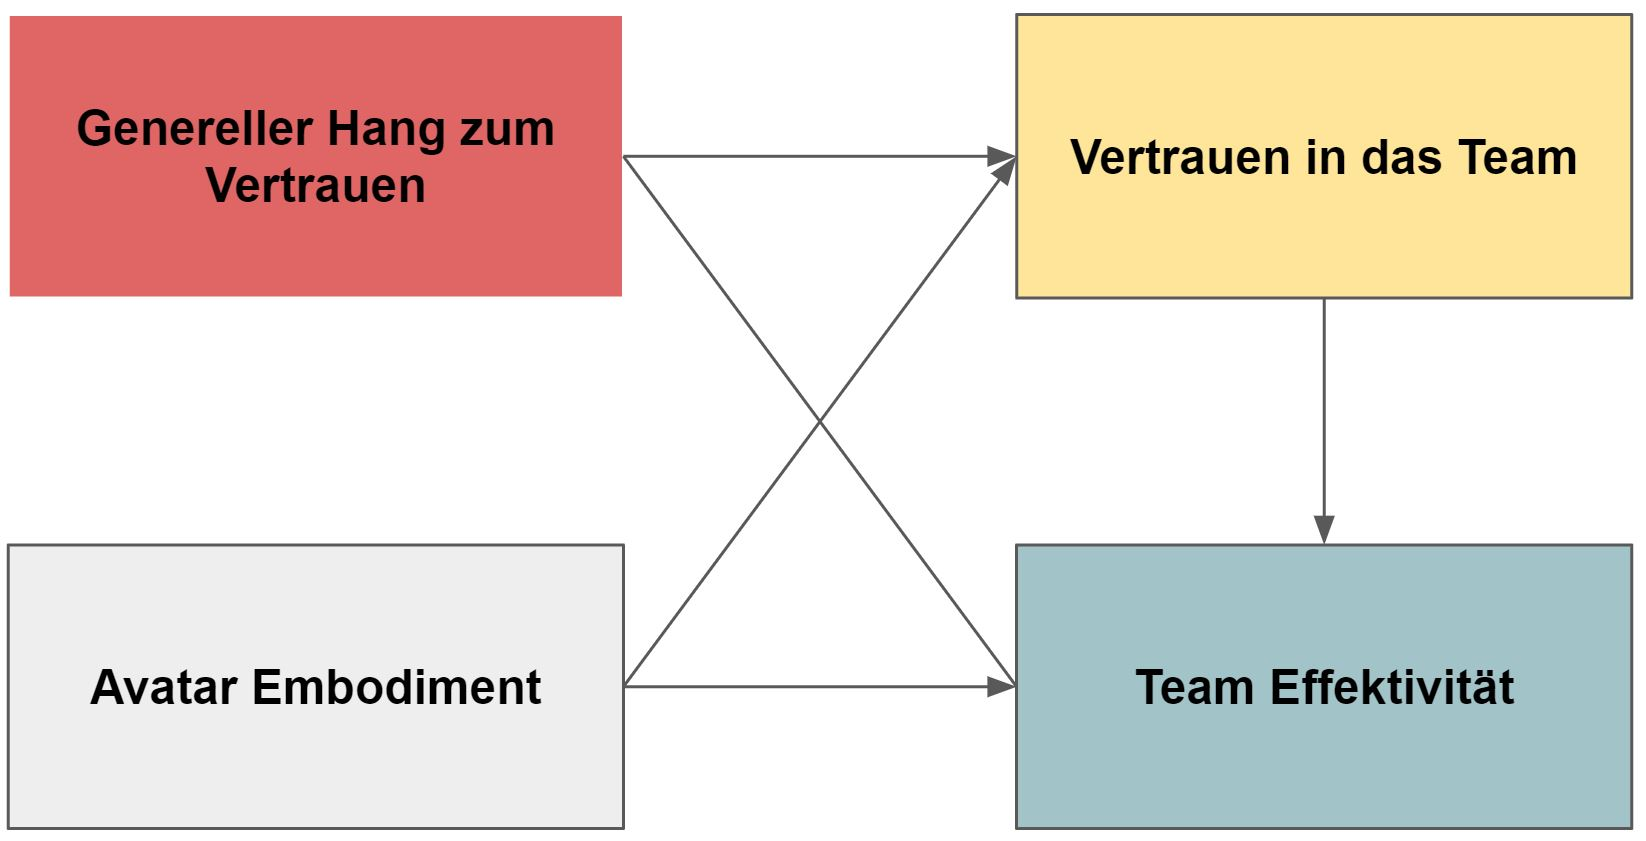
\includegraphics[width=\textwidth]{Abbildungen/Framework_02.JPG}\\
			\caption[Abbildung 1]{Das Framework}
			\label{Framework}
		\end{footnotesize}
	\end{figure}

Da dieses Framework nicht validiert ist, kann es sein, dass die verschiedenen Faktoren nicht zu gleichen oder auch gar keinen Einfluss auf die Team-Effektivität haben.
%
%Grundlage für das Framework \autoref{Framework} sind verschiedene wissenschaftlich basierten Quellen, die sich mit der \ac{vr} sowie zwischenmenschlichem Vertrauen befassen. Diese beiden Teilbereiche wurden kombiniert und soll versuchen, die Team-Effektivität anhand variierendem zwischenmenschlichen Vertrauen und verschiedenen Avatar-Verkörperungen zu messen.
%
%Wie an dem Framework zu erkennen ist, wird davon ausgegangen, dass die beiden Faktoren \dq{}Generelles Vertrauen\dq{} sowie \dq{}Vertrauen in das Team\dq{} das \dq{}Zwischenmenschliche Vertrauen\dq{} zu gleichen Teilen beeinflussen. 
%
%Weiterhin hat die Kombination des \dq{}Avatar-Embodiment\dq{} sowie des \dq{}Zwischenmenschlichem Vertrauen\dq{} ebenfalls einen Einfluss zu gleichen Teilen.
%
%Da dies jedoch das erste mal ist, dass dieses Framework theoretisch Aufgestellt wurde, kann es sein, dass die verschiedenen Faktoren nicht zu gleichen oder auch gar keinen Einfluss auf die Team-Effektivität haben.

	\newpage
\section{Grundlagen}

%\subsection{Team und Gruppen}

	\subsection{Virtual Reality}
	\label{Virtual Reality}
%		\subsubsection{VR - Wozu brauchen wir Virtual Realitky?}
		\subsubsection{VR - Virtuelle 3D-Welten}
Virtual-Reality ist eine Realität, die durch den Computer, geschriebenen Computercode sowie erstellte 3D-Welten, abgebildet und zum Leben erweckt wird. Dabei Spielt der Nutzer, das umschließende Erlebnis sowie die Interaktivität in der \ac{vr}, eine Zentrale Rolle. \citep[p.6-12]{sherman2018understanding}
	Seit vielen Jahren sind \ac{sve}'s Forschungsgrundlage der Virtuellen Realität. Siehe \citep{shuffler2011there} \citep{steed1999leadership} und \citep{de2011level} \\
	\ac{sve}'s bieten die Möglichkeit, geographisch getrennte Personen in einer virtuellen Umgebung zu verbinden. Dadurch wird den Nutzern der virtuellen Realität die Möglichkeit bereit gestellt miteinander zu kommunizieren und zu interagieren. \citep[p. 1-3]{pettifer1999designing} Eine gute Übersicht der Anwendungsgebiete eines \ac{sve} wurde von Richard Waters dargestellt. Siehe \citep{waters1997rise}.
	Zur Durchführung und zur Datenerhebung dieser Studie wurde ein \ac{sve} entwickelt, welches den Nutzern ein \dq{}Hand- und Kopf getrackten Avatar\dq{} (\ac{ik}) oder ein \dq{}Hand-, Kopf und Inverskinematisch-simuliertem Torso getrackten Avatar\dq{} (\ac{nik}), je nach Anwendungsfall, zur Verfügung stellt. Innerhalb des \ac{sve} können sich die Nutzer frei bewegen, andere Avatare Wahrnehmen und mit diesen interagieren.
	
	
		\subsubsection{VR - Vorbedingungen für Presence}
Um die bestmöglichste Umschlossenheit in einer \ac{vr} zu erreichen, wird eine Schnittstelle zur Interaktion zwischen den Sinnen und der Außenwelt benötigt. Dies kann ein \ac{hmd} sein, welches ein computergeneriertes Bild erzeugt, durch das die \ac{vr} wahrgenommen werden kann. Darüber hinaus muss das \ac{hmd} in der Lage sein, den Kopf des Benutzers frei im Raum zu Verfolgen und die gewonnenen Positionsdaten auf die \ac{vr} abzubilden. Optimalerweise werden Controller benötigt, durch deren Einsatz es möglich ist, auch die Handbewegungen der realen Personen zu Verfolgen und die gewonnenen Positionsdaten in der \ac{vr} darzustellen. Das \ac{hmd}, die Controller, eventuelle zusätzliche Körpertracker, Kopfhörer, eventuell wahrgenommener Geruch etc. definieren, zu welchem Ausmaß Sinnesmodalitäten in der \ac{vr} generiert werden können. Der Grad der Immersion hängt somit direkt mit der Anzahl der angesprochenen Sinnesmodalitäten zusammen. Je mehr Sinnesmodalitäten auf einmal angesprochen werden, desto mehr ist der Wahrnehmungsapparat in der Lage, die virtuelle Umgebung auf die reale Welt abzubilden. \\
Somit lässt sich sagen, dass die Voraussetzungen um \dq Presence\dq{} zu erreichen in der \ac{vr} die Korrelation zwischen den Sinneseindrücken, der Propriozeption und dem Grad der wahrgenommenen Realität der Illusion, sich in einem stabilen räumlichen Ort zu befinden, darstellt. Sind diese Voraussetzungen gegeben, kann der Nutzer einen plausiblen Vergleich zwischen realen sensorischen und virtuellen, durch Illusion erzeugten Daten, aufstellen. Vgl. \citep{slater2009we}

		\subsubsection{VR - Presence in Virtual Reality}
			
	Dank heutiger Technologien ist es uns möglich, zu jeder Zeit mit Personen an verschiedenen Orten zu interagieren und zu kommunizieren. Kommunikation nicht mehr nur auf die Personen in unserer unmittelbaren Umgebung beschränkt. 
	Das Voranschreiten der Technologie ermöglicht es, uns nicht mehr nur auf soziale Interaktionen mit physischen Wesen zu beschränken, sondern erweitert diese auch auf Repräsentationen geschaffen aus Pixeln, E-Mails, Film oder durch das Telefon. Je nachdem, wie Stark diese Repräsentation von uns Wahrgenommen wird, schafft Sie es, kraftvolle Emotionen in uns auszulösen.\citep[p. 4-6]{biocca2002defining}\\
	Nur wenn eine gewisse \dq Presence\dq{} dieser Repräsentation besteht, kann \textbf{Vertrauensbildung} funktionieren. Somit definiert das Vorhandensein des Gefühls von \dq Presence \dq{} den Grundbaustein für alle weiteren Schritte.\\
	Der Begriff \dq Presence\dq{} ist nicht genau definiert. Am ehesten trifft die Beschreibung zu, dass \dq Presence\dq{} das subjektive empfinden ist, an einem anderen Platz zu sein, obwohl man physikalisch eigentlich woanders ist. \citep[p. 1]{witmer1998measuring} 

	Wenn eine Person eine andere Person in einer \ac{ivr} als Präsent wahrnimmt, werden die Wahrnehmenden, vestibulären, propriozeptiven und autonomen Nervensysteme in einen Zustand gebracht, der einem realen Zustand gleicht. Obwohl die betroffene Person weiß, dass Sie sich nicht in einer realen Lebenssituation befindet, wird diese dazu neigen, sich so zu verhalten, als ob diese in einer ist und ähnliche Gedanken und Gefühle haben. \citep{slater2003note}

Diesbezüglich kann \dq Presence\dq{} als eine Art von Illusion angesehen werden, da die erzeugte Stimuli in der \ac{vr}, wie in der Realen Welt auch auf unsere Rezeptoren projiziert werden.

Somit lässt sich \dq Presence\dq{} in der \ac{vr} in 4 verschiedene Teilbereiche unterteilen.

\begin{itemize}
	\item{Die Illusion, sich in einem stabilen räumlichen Ort zu befinden} : Alle Stimuli zur räumlichen Wahrnehmung - wie zum Beispiel keine Restriktionen des \ac{fov} \footnote{Sichtfeld}, keine Kabel am \ac{hmd} - sollten sich möglichst wie in der realen Welt verhalten. \citep[p.47]{jerald2015vr}
	\item{Die Illusion der Selbstverkörperung} : Beschreibt das Gefühl einen Körper in der virtuellen Umgebung zu haben. Studien fanden heraus, dass durch einen virtuellen Körper die \dq Presence\dq{} in der \ac{vr} stark steigt. \citep[p.756]{botvinick1998rubber} Der virtuelle Körper muss nicht unserem eigentlichem ähnlich sehen. \citep[p.7]{maxwell1960psycho}
	\item{Die Illusion von körperlichen Interaktionen} : Beschreibt beispielsweise das vorhanden sein von Audio Feedback oder die Vibration des Controllers. Diese Kleinigkeiten tragen eine große Menge dazu bei, \dq Presence \dq{} in der \ac{vr} zu steigern. \citep[p.48]{jerald2015vr}
	\item{Die Illusion von sozialer Kommunikation} Sozialer-Realismus kann vom Physischen-Realismus abgetrennt werden. Social-Presence beschreibt das Gefühl, wirklich mit jemandem in einem \ac{sve} zu kommunizieren. Sei es verbal oder durch Körpersprache. Je mehr Nutzer der virtuellen Welt sich so verhalten, als ob diese real wäre, desto mehr steigt auch die \dq Social-Presence\dq{}. \citep[p.49]{jerald2015vr} \citep[p.12]{guadagno2007virtual}
\end{itemize}

%\begin{figure}[H]
%		\begin{footnotesize}
%		\centering
%			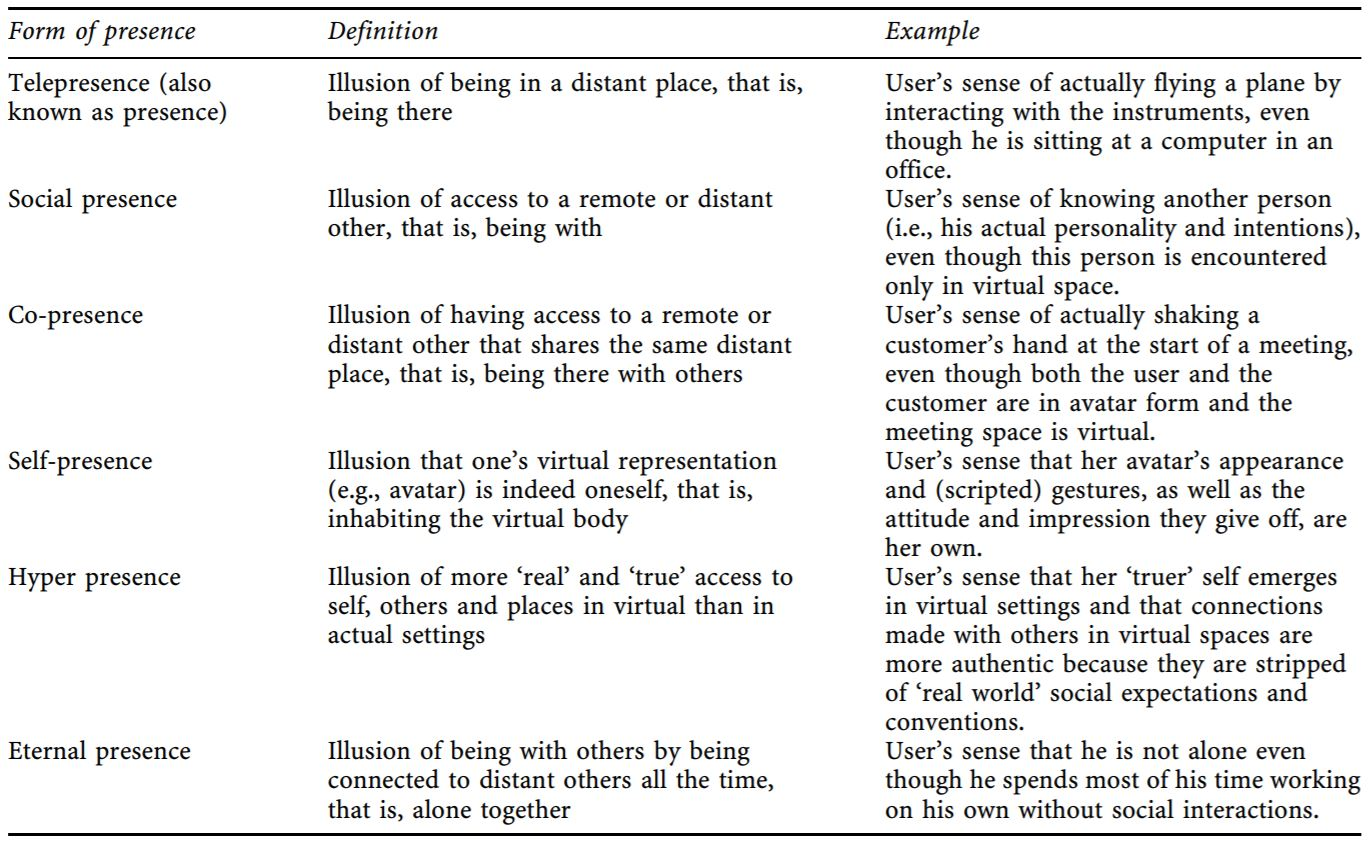
\includegraphics[scale= 0.4]{Abbildungen/forms_presence.JPG}
%			\caption[Abbildung 1]{Forms of Presence}
%			\textit{Die Verschiedenen Formen von Presence laut U.  Schultze \citep{schultze2010embodiment} }
%			\label{vertical_horizontal}
%		\end{footnotesize}
%	\end{figure}


\dq Presence\dq{} ist ein Konstrukt aus Immersion und dem Nutzer. Immersion kann ein Gefühl von \dq Presence\dq{} erschaffen, muss es aber nicht zwangsläufig. Je Immersiver ein \textbf{System} ist, desto höher ist das Potential dieses Systems, dass der Nutzer ein Gefühl von \dq Presence\dq{} entwickelt.
			
Dementsprechend unterscheidet Lombard 6-Arten von \dq Presence\dq{} :
	\begin{itemize}
		\item \textbf{Sozialer Reichtum} : Das Medium wird als empfindlich oder persönlich wahrgenommen, wenn es zur Interaktion mit anderen Menschen verwendet wird.
		\item \textbf{Der Realismus} : Beschreibt die Wahrnehmung oder/und den Realismus der \dq Presence\dq{} und bis zu welchem Grad dieser als "Real" dargestellt werden kann.
		\item \textbf{Das Transportmedium} : Dies beschreibt das Gefühl "Du bist da", "Es ist da", oder/und "Wir sind Zusammen".
		\item \textbf{Die Immersion} : Beschreibt, wie Flächendeckend die Sinne des Benutzers angesprochen werden.
		\item \textbf{Der soziale Akteur innerhalb des Mediums} : Beschreibt die Reaktion auf eine Repräsentation einer Person durch ein Medium, auch wenn diese Irrational begründet ist.
		\item \textbf{Das Medium als sozialer Akteur} : Beschreibt die Situation wo der Akteur ( z.B. Computer ) selber als ein soziales Wesen wahrgenommen wird.					
				\citep{lombard1997heart}
			\end{itemize}
			
Um Vertrauen optimal aufbauen zu können, sollte das gesamte \ac{sve} so real wie möglich abgebildet sein. Diesbezüglich richtet sich diese Arbeit an nahezu alle Arten der hier genannten \dq Presence \dq{}.

%Telepresence
%Co-Präsenz
%Selbst wahrgenommene Copräsenz
%Others Co-Präsenz
%wie im Fragebogen halt!

%https://scihubtw.tw/10.1057/jit.2010.25

%Telepresence
%Telepresence is the origin of the concept of presence as
%adopted by most of the research on virtual environments.
%The prefix ‘tele’ was initially used to signal the conceptualization of presence in a computer-mediated rather than a
%physical environment (Lee, 2004). The term telepresence
%was coined by NASA and the robotics community to refer
%to the illusion of being transported via telecommunication
%systems to a real, physical location, which could then be
%experienced synchronously from afar (Minsky, 1980).
%Over time, the meaning of telepresence was relaxed to
%include virtual settings also, especially single-user VR.
%Soon the prefix was dropped or adapted. For instance,
%what was previously labeled telepresence, namely the
%perceptual illusion of ‘being there’ in the virtual setting
%(Biocca, 1997), became merely ‘presence’ or virtual,
%physical, spatial, mediated and subjective personal presence (Heeter, 1992; Ijsselsteijn et al., 2001), to name a
%few. Some of these descriptors were technology specific.
%For instance, virtual presence was used to define presence
%in virtual environments specifically. Others were related
%to the diverse disciplinary backgrounds of the researchers from computer science, business, IS, engineering,
%education and psychology, who were attracted to the interdisciplinary research into computer-mediated environments (Lee, 2004). For instance, applying a cognitive
%lens to their study of presence, Regenbrecht and Schubert
%(2002) coined the term spatial presence to separate the
%user’s mental representation of his body being part of the
%virtual space from the attentional component of presence,
%namely involvement.
%
%Social presence
%If telepresence is the illusion of being in a distant place
%(being there), then social presence is the illusion of access
%to a remote or distant other (being with). Even though
%social presence was originally conceptualized as a property
%of the communication medium (Lombard and Ditton,
%1997), specifically the medium’s ability to increase others’
%salience in an interaction (Short et al., 1976), in the
%research on virtual environments, social presence became
%a psychological construct that reflected the subjective
%experience of closeness to and connectedness with others
%in mediated communication (Biocca, 1997). This definition
%seems appropriate given the more social nature of persistent virtual environments such as MUDs. Compared to
%media like bulletin boards, web pages and blogs, virtual
%worlds required synchronous presence (Kolko, 1999). As
%such, the focus of social presence increasingly moved to
%the user’s experience of virtual others, leading Blascovich
%(2002, p. 130) to defines it as ‘a psychological state in which
%the individual perceives himself or herself as existing within
%an interpersonal environment’.
%Avatars, with their ability to convey social cues, are
%deemed to enhance social presence, in that they convey
%agency (i.e., control by human means) and behavioral
%realism (Blascovich, 2002). As such, they make an expanded
%definition of social presence possible, namely one that
%relies on the user’s access to the other’s intelligence so as to
%read the other’s mind and infer his intentional states
%(Biocca et al., 2003). Bente et al. (2008) thus conceptualize
%social presence as a multi-dimensional continuum, wherein
%low social presence pole denotes the communicator’s sense
%of spatial co-presence and high social presence is associated
%with gaining access to others’ intentional, cognitive and
%affective states. Bente et al. (2008) found that high levels of
%social presence correlated significantly with interpersonal
%trust.
%Social presence can apply to both human and non-human
%forms of intelligence, either real or imagined (Biocca, 1997).
%To the extent that these real or imagined others (e.g., people,
%animals, fantastical creatures or robots) populate the virtual
%world and react to the communicator, she is assured that she
%and the world exist (Heeter, 1992). If the individual is
%ignored, doubts about her and the world’s existence are likely
%to arise. Social presence thus supports an individual’s sense
%of ‘being there.’

%Co-presence
%If telepresence focuses on being there (in a space), and
%social presence focuses on being in the presence of real or
%imagined others, then co-presence is the sense of being in a
%shared virtual setting with remote others (Ijsselsteijn et al.,
%2001). As such, co-presence is conceptualized at the intersection between tele- and social presence. It is the virtual
%equivalent to Goffman’s (1959) definition of co-presence as
%collocation of embodied – not merely imagined – others
%that become available and accessible to each other. This
%form of presence is made possible by shared virtual
%environments.
%Durlach and Slater (2000), who refer to co-presence as
%virtual togetherness, view it as the socially shared counterpart to an individual’s experience of (tele)presence. One key
%determinant of co-presence is the ability to touch virtual
%others and to jointly manipulate shared space and shared
%objects (e.g., documents). Unlike audition and vision, touch
%requires proximity. To the extent that one person’s actions
%affected by touching people, things and spaces in the environment are clearly perceived by the other participants,
%co-presence is enhanced (Durlach and Slater, 2000).

%Self presence
%Self presence derives from our experience of ourselves in
%everyday life (Goffman, 1959). In persistent virtual environments in particular, this experience of the self can become
%virtual when the user is represented through an avatar or,
%as in first person shooter games, a hand or gun. Lee (2004)
%maintains that self presence occurs when users do not
%notice the virtuality of the representation of their own
%selves. In other words, self presence is high when users
%inhabit their avatar and feel no distinction between themselves and their digital representation (also Eastwick and
%Gardner, 2008; Gee, 2008).
%In his conceptualization of self presence, Biocca (1997)
%highlights that the whole concept of presence in virtual
%worlds is only possible because of the distinction users
%make between their actual/physical, their virtual/avatar and
%their phenomenal bodies. The phenomenal body is the
%user’s mental model or schema of her body. It consists of
%perceived shape, size and capabilities, among other bodily
%attributes. Self presence is the users’ mental model of
%themselves inside the virtual world; it is their awareness of
%self-identity. As such, it plays an important role in users’
%self-discovery, which in turn shapes their mental model.


		\subsubsection{VR - Presence und Co-Presence}
Wenn Personen sich zusammen in einer \ac{ivr} befinden und die andere Person wahrnehmen, wird dieses Gefühl mit  \dq Co-Presence bzw. Social-Presence\dq{} bezeichnet. \citep{schuemie2001research}\\
\textbf{\dq Co-Presence\dq{}} bezeichnet das Gefühl, mit einer anderen Person in Verbindung zu stehen.
Es wird die Anwesenheit der anderen gespürt und es wird wahrgenommen, dass die andere Person ebenfalls spürt, dass man Selbst anwesend ist. 
Co-Presence dementsprechend als eine psychologische Verbindung \textit{zu und mit} dem anderem Charakterisiert werden.  \\
Fühlt sich ein Nutzer einer \ac{ivr} \dq{}innerhalb\dq{} des Mediums \ac{vr}, so wird dies als \textbf{Telepresence} bezeichnet. Telepresence bezeichnet das Gefühl \dq{}da zu sein\dq{}. Je höher das Level wahrgenommener Telepresence ist, desto weniger fühlt sich der Nutzer an dem Ort seines physikalischem Körpers und mehr an einem anderem Ort. \citep[p.482]{nowak2004effect}\\
Der Begriff der \dq{}\textbf{Social-Presence} \dq{} beschreibt, wie stark ein Nutzer eine Person, mit der dieser nur mittels Kommunikationstechnologie kommuniziert, als \dq{}real\dq{} bezeichnet. Social-Presence wird dabei auf die Kommunikationstechnologie an sich bezogen. Je mehr Social-Presence vorhanden ist, desto besser ist ein Kommunikationsmittel geeignet um Informationen über den Interaktionspartner zu übermitteln. So erzeugt ein Videochat durch die zusätzliche Übertragung eines Videos mehr Social-Presence als eine Telefonkommunikation.  \citep[p.151]{gunawardena1995social}
Es wird davon ausgegangen, dass eine \ac{sve}'s mehr Social-Presence erwecken kann als Beispielsweise ein Telefonat. Dies sei damit begründet, dass \ac{sve} die Eigenschaften und Interaktionen des anderen besser darstellen und einfangen kann. Desto mehr Eigenschaften einer Person dargestellt werden können, desto höher ist der wahrgenommene Realitätsgrad des anderen. \citep[p. 5-8]{biocca2002defining}
Somit reicht das gesamte Kontinuum der Presence von der räumlichen Komponente bis hin starken psychiologischen Beteiligungen. Dies macht es möglich, auch auf die affektiven und kognitives Zustände von Personen aufzudecken. Höhere wahrgenommene Presence führt dazu, dass die Person sich mehr mit der \ac{vr} engagieren kann, was zu Handlungen führt, die als verbunden und voneinander abhängig wahrgenommen werden. \citep{biocca2001criteria}
		\subsubsection{VR - Presence und Teambuilding}

\newpage

\subsection{Avatare}
\label{Avatare}
\subsubsection{AVATARE - Repräsentationen von Avataren}

Das Menschliche Gehirn ist in der Lage, computergenerierte Darstellungen in \dq{}Lebend und Nicht-Lebend\dq{} zu kategorisieren. Einige Forschungen gehen davon aus, dass das menschliche Gehirn semantische Unterschiede im Zusammenhang mit der \dq{}Social-Presence\dq{} feststellen kann. So kann eine menschenähnliche Form als biologisch oder nicht-Lebend erkannt werden. 

	\begin{figure}[H]
		\begin{footnotesize}
		\centering
			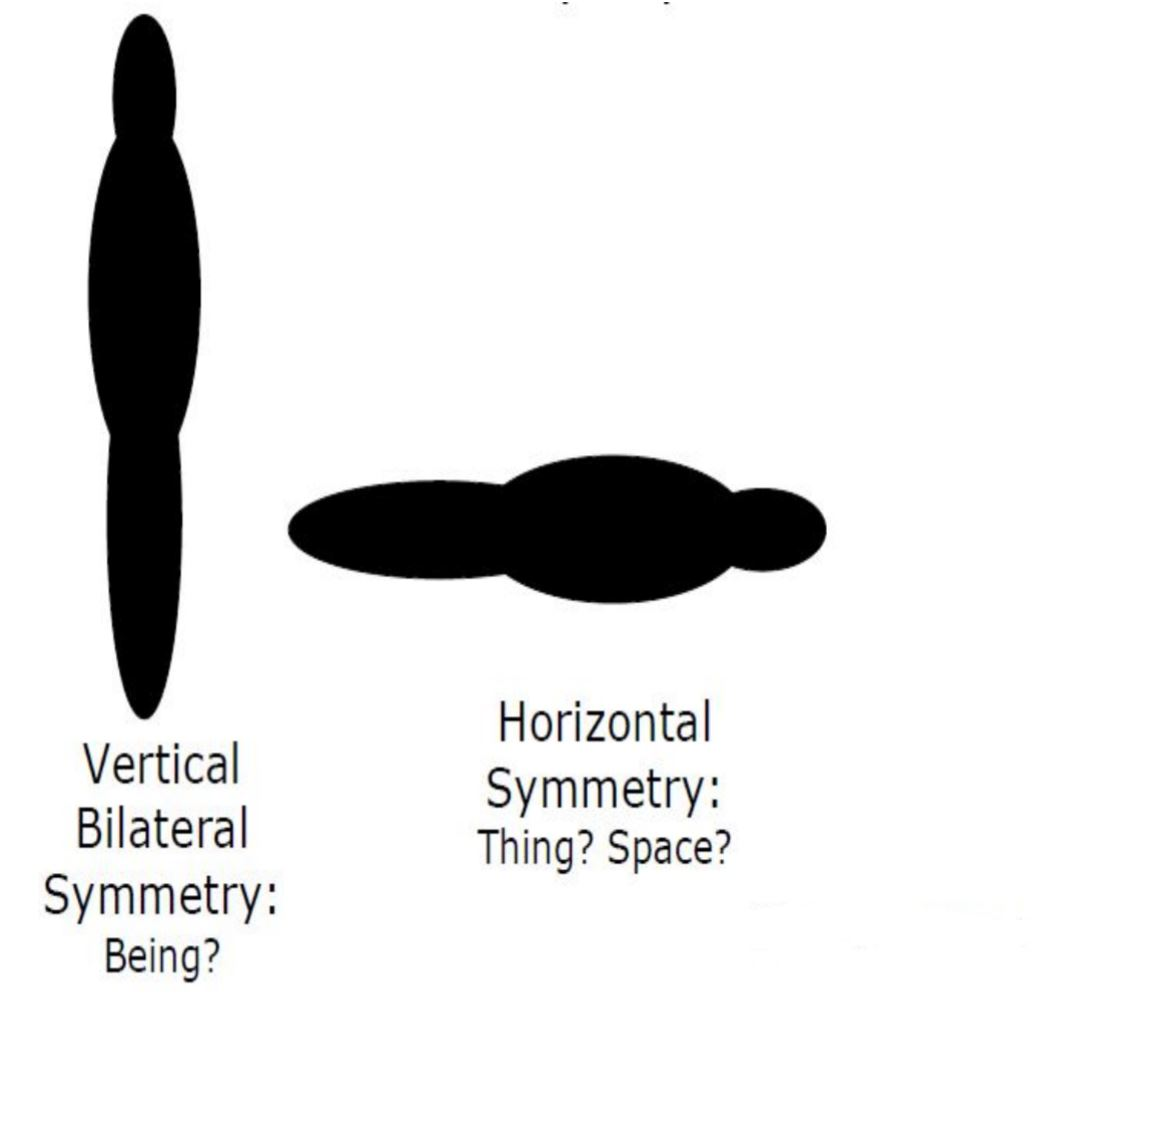
\includegraphics[scale= 0.3]{Abbildungen/Symmetry.JPG}
			\caption[Abbildung 1]{Social presence response to vertical and
horizontal beings}
			\textit{Menschen interpretieren symmetrische Formen um eine vertikale Achse eher als \dq{}Menschlich\dq{} als Formen um die horizontale Achse. \citep{biocca2002defining} }
			\label{vertical_horizontal}
		\end{footnotesize}
	\end{figure}

In \autoref{vertical_horizontal} ist zu erkennen, dass eine menschenähnliche vertikale, bilateral Symmetrische Repräsentation mehr \dq{}Co-Presence\dq{} erweckt als die horizontale bilateral Symmetrische Repräsentation. \citep[p.546-551]{thornhill1998relative}
Bilateral-Vertikale Symmetrie wird mit der körperlichen Gesundheit eines Menschen in Verbindung gebracht. Sogar Weibchen verschiedener Spezies neigen dazu, Partner mit einem höheren Grad an bilateraler Symmetrie für die Fortpflanzung auszuwählen. \citep[p. 659–669]{rhodes1998facial} \citep{biocca2002defining} \citep[p.233–242]{grammer1994human} \ \\

\begin{figure}[H]
		\begin{footnotesize}
		\centering
			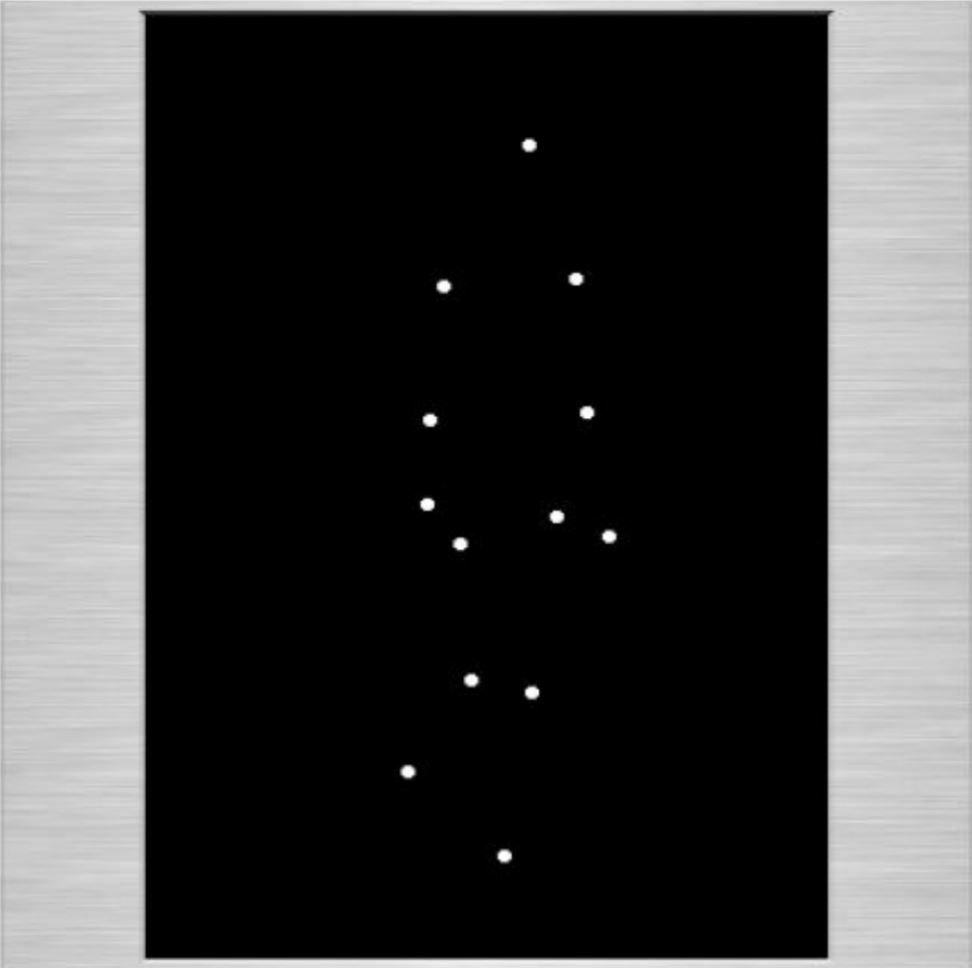
\includegraphics[scale= 0.5]{Abbildungen/moving_dots.JPG}
			\caption[Abbildung 1]{Social presence response to vertical and
horizontal beings}
			\textit{Stationäre punkte, bei denen der Mensch eine lebendige Bewegung ausmachen kann, wenn diese Anfangen sich zu bewegen. Es ist sogar möglich einen Menschen zu erkennen, dessen Art der Aktivität sowie den emotionalen Zustand. \citep{biocca2002defining} \citep[p.76-89]{johansson1975visual}}

			\label{moving_dots}
		\end{footnotesize}
	\end{figure}

Schon sich nur bewegende Punkte können als intelligente Wesen wahrgenommen werden. Johannson \citep[p.76-89]{johansson1975visual} führte eine Studie durch, in der die Teilnehmer dreizehn \autoref{moving_dots} sich bewegende Punkte sahen und sofort die Darstellung einer menschlichen Bewegung erkannten. Als die Teilnehmer Punkte sahen, die stationär waren, ist es ihnen nicht möglich gewesen, diese Punkte als menschliche Repräsentation zu erkennen. Wenige Punkte reichen aus, um Informationen zu erzeugen, die Aufschluss über die Aktivität, das Geschlecht, die Bewegung, den emotionalen Zustand oder die Anzahl der Personen zu geben.

		\subsubsection{AVATARE - Selbst-Avatar und Nicht-Selbst-Avatare}

In der \ac{vr} und in einigen anderen computerbasierten Medien, kann der Nutzer sich Avatare erstellen und mit diesen interagieren. Ein Avatar bezeichnet eine Grafikfigur, die die Onlinerepräsentation eines Nutzers in einer Virtuellen Umgebung darstellt. \citep[p.1]{neustaedter2009presenting} \\
\ac{hmd}'s beeinflussen das Sichtfelds des Nutzers so stark, dass diese Ihre eigenen Körper nichtmehr sehen können. Um diesem Nachteil entgegenzuwirken, kann einem Nutzer ein virtueller Körper zur Verfügung gestellt werden. Dieser Körper wird Selbst-Avatar genannt.
Es ist schwierig einen Selbst-Avatar hoher Qualität zu simulieren. Dazu wäre im Idealfall das Verfolgen und Animieren mehrerer Körperteil unabdingbar. Ist der Selbst-Avatar schlecht animiert oder es entstehen während der Nutzung Trackingfehler, die der Nutzer erkennt, kann sehr leicht zu einem \ac{bip} kommen. Bei diesem \ac{bip} bricht die gesamte Illusion der \ac{vr} für den Nutzer in sich zusammen. 
Dies ist auch der Grund, weshalb relativ wenige \ac{vr}-Anwendungen einen menschlichen Körper als Avatar darstellen.
Sind jedoch genügend Körperteile getracked und animiert, muss der Avatar nicht unverwechselbar menschlich aussehen um einen glaubwürdigen Selbst-Avatar zu vermitteln. Selbst grobe Avatar-Darstellungen schaffen es, ausreichende Informationen über die Glaubwürdigkeit eines menschlichen Körpers zu Vermitteln. \citep{lok2003effects}

Biocca forschte Umfangreich über den Einfluss von Self-Avataren auf den Nutzer in der \ac{vr}. \citep[421-427]{construal2014connected} 
\newline So beispielsweise, wie sich die Interaktion mit der Welt verändert, wie sich soziale Interaktionen verändern und wie Aufgaben wahrgenommen und erledigt werden. \citep{benford1995user} \citep{bowers1996talk}
Bioccas Studien gehen davon aus, dass ein menschenähnlicher Körper als Avatar die Self-Presence stark erhöht. Um die Self-Presence noch stärker zu erhöhen, wird ein Inverse-Kinematisch simulierter Avatar als Self-Avatar genutzt werden.

Die Ursprünge der Inverse-Kinematic liegen in der Robotik. Es geht darum, herausfinden, wie Gelenke eines Roboterarms bewegt und gedreht werden müssen, um Beispielsweise einen Gegenstand von Punkt A nach Punkt B zu bewegen. Dies ist besonders Sinnvoll bei Self-Avataren in einem \ac{sve}. Inverse-Kinematische Berechnungen können nicht nur auf Arme angewandt werden, sondern auch auf den Torso, die Füße, den Kopf, die Beine, etc.. Benutzt ein Nutzer in einem \ac{sve} einen Inverse-Kinematisch dargestellten Self-Avatar, kann dieser Beispielsweise die Torsorotation, Armbewegungen oder Beinbewegungen des eigenen Avatars sehen.

Yee und Bailenson fanden heraus, dass die Selbst-Presence Einfluss auf den Proteus-Effekt hat. Je stärker die Selbst-Presence eines Nutzers, desto stärker ist auch der Proteus-Effekt. Der Proteus-Effekt beeinflusst den Nutzer so, dass sozialen Interaktionen des Nutzers denen der sozialen Identifikation seines Avatars ähneln. So nimmt eine Person, das Verhaltensmuster entsprechend zu dem Aussehen des Avatars ein. Je nachdem, wie der Nutzer glaubt, dass bestimmte Verhaltensweisen von ihm, aufgrund des Avatars, erwartet werden. \citep{ratan2015leveling} 
Diese Abbildung der Verhaltensweisen lässt sich auch auf den Gruppenkontext beobachten. Der Nutzer wird sich in einer Gruppe so Verhalten, wie die Gruppenkonformität es vorgibt.
Dieser Effekt kommt nicht nur bei unverwechselbar Menschenähnlichen Avataren vor, sondern kann auch bei anderen Avatararten auftreten. Solche identitätsbezogenen Avatar-induzierten Effekte, können die \dq{}Kognitiven-Einstellungen\dq{} (siehe Kapitel \textit{\nameref{Vertrauen}}) und Verhaltensweisen anderer Personen gegenüber beeinflussen. \citep{lok2003effects}

Weiterhin wurden zahlreiche weitere Forschungen durchgeführt, um den Einfluss von Avataren zu erforschen. So gibt es Experimente, die den Einfluss des Geschlechts \cite{slater2010first}, der Hautfarbe \cite{peck2013putting} oder des Grades des Realismus \cite{roth2016avatar}, als Inhalt ihrer Forschungen haben.

Es stellt sich die Frage, ob ein Avatar menschenähnlich Aussehen sollte. Diese Frage stellten sich George, Eiband, Hufnagel und Hussman \cite{george2018trusting} in Ihrer Forschung und verglichen, ob sich mehr Vertrauen zwischen einem Menschenähnlichem oder einem Roboterartigen Avatar aufbauen lässt.
Dazu schufen Sie ein Szenario, in dem Probanten mittels eines \ac{hmd}, ein Social-Dilemma-Scenario \footnote{Situationen, in denen - die rationale Verfolgung von Eigeninteressen zu einer kollektiven Katastrophe führen kann} erlebten. Sie fanden keinen signifikanten unterschied in der Vertrauenswürdigkeit zwischen Menschenähnlichen und Roboterartigen-Avataren. Jedoch wurde ein größeres Gefühl von Zusammenheit festgestellt, wenn mit einem Menschenähnlichem Avatar interagiert wurde. \citep{kerr1983motivation}
Sie erwähnten weiterhin in Ihrer Studie, dass gute Grafik und Realistisches Verhalten durch beispielsweise Mikrogestikulationen, soziale Interaktionen sowohl die Co-Presence fördern. \citep{george2018trusting}

Um den den Einfluss des Grades des Realismus unter Avataren zu erforschen, führten Riedl, Mohr und Kenning \cite{riedl2014trusting} eine Studie zum Vertrauensaufbau unter Menschen im Vergleich zu Avatare mit menschenähnlichen Gesichtern, durch. Sie fanden heraus, dass es Personen leichter fällt einzuschätzen, dass eine reale Person, im Gegensatz zu einem Avatar mit menschenähnlichen Gesicht, vertrauenswürdig ist. Es wurde der Frontalkortex - die Gehirnregion, der dafür Verantwortlich ist einzuschätzen, wie die Gedanken und Gefühle des gegenüber sind - bei Interaktionen mit Menschen mehr angeregt, als bei Interaktionen mit Avataren mit menschenähnlichen Gesichtern.
Jedoch ist die Lernrate des Vertrauensaufbau zwischen Menschen und Avataren gleich. Somit wird Vertrauen zwischen Menschen in der gleichen Geschwindigkeit aufgebaut wie zwischen Avataren. \cite{riedl2014trusting}

Somit lässt sich feststellen, dass ein höherer Grad an Realismus den Vertrauensaufbau fördert, jedoch kein signifikanter Unterschied zwischen einem menschenähnlichem sowie Roboterähnlichem Avatar besteht. Diese Vermutung bestätigten auch Bente, Rüggenberg und Krämer \citep[p.54-59]{bente2004social} indem sie eine Studie zur Social-Presence von Avataren in einem \ac{sve} durchführten. Das \ac{sve} war ähnlich einer Videokonferenz aufgebaut. Es waren keine \ac{hmd}'s vorhanden und die Teilnehmer haben sich während des Experiments nicht gesehen. Sie verglichen die Kommunikationarten, Face-to-Face, Chat und Avatarbasierte Kommunikationsmedien untereinander, um Unterschiede in der Social-Presence sowie dem zwischenmenschlichen Vertrauen festzustellen.
Es wurde festgestellt, dass wenig Kognitives-Vertrauen während der Nutzung des \ac{sve} zu Avataren aufgebaut werden konnte, während Face-to-Face, Telefon und Chatkommunikationen besser abschnitten. Weiterhin wurde weniger Affektives-Vertrauen im \ac{sve} als bei der Telefon oder Face-to-Face kommunikation aufgebaut.
Bente, Rüggenberg und Krämer \citep[p.54-59]{bente2004social} gehen davon aus, dass dies mit der Neuheit der Technologie zusammenhängt.

Da in dieser Studie lediglich die beiden Controller sowie das \ac{hmd} getrackt werden, wurde sich dazu entschieden, keine Darstellung eines Selbst-Avatars zu wählen. Stattdessen sehen die Nutzer des \ac{sve} menschenähnliche Hände \underline{ohne} ihre Extremitäten. Die Avatare, die von den anderen teilnehmenden Personen angenommen werden, können jedoch einen Körper besitzen. In dieser Studie wurde dafür zwischen der Kondition \ac{ik} sowie \ac{nik} der Avatare unterschieden.

%Connected to My Avatar:
%Effects of Avatar Embodiments on User Cognitions, Behaviors,
%and Self Construal 
%
%421
%https://sci-hub.do/10.1007/978-3-319-07632-4 
%file:///B:/Chrome%20Downloads/Biocca2014_Chapter_ConnectedToMyAvatar.pdf 


%Emotional Contagion with Artificial Others. Effects
%of Culture, Physical Appearance, and Nonverbal Behavior
%on the Perception of Positive/Negative Affect in Avatars 	

%412

%https://sci-hub.do/10.1007/978-3-319-07632-4
	

%https://dl.acm.org/doi/fullHtml/10.1145/223904.223935?casa_token=B8tEKM39OVQAAAAA:VNilOxaXG3_2Bw-bEClS10xyOXLBxB8ymyo4B-d1kUoAmCgWC1MDdVKSptRADsBaGw19nzE15dwIWQ

%http://mcneilllab.uchicago.edu/pdfs/dmcn_vietri_sul_mare.pdf

%https://sci-hub.ren/https://doi.org/10.1371/journal.pone.0025759 SEITE 2


\newpage

	\subsection{Vertrauen}
	\label{Vertrauen}
Der Begriff \textbf{Vertrauen} ist in viele Bereiche des alltäglichen Lebens eingezogen. Er beschreibt ein Psychologischen Konzept, dass jeden Menschen ständig begleitet.
Ein Politiker wirbt um das Vertrauen seiner Wähler, Unternehmer beschreiben sich selbst als Geschäftspartner des Vertrauens oder es \dq wird der Arzt des Vertrauens\dq empfohlen.

Vertrauen in die \ac{vr} kann auf zwei unterschiedliche Art und Weisen betrachtet werden. Das Vertrauen in die \ac{vr}-Technologie sowie das zwischenmenschliche Vertrauen, das in der \ac{vr} zwischen 2 oder mehreren Personen gebildet wird.
%Mangelndes Vertrauen in eine Technologie, kann Nutzer dran hindern, diese zu Nutzen. \citep{trustInVRTechnology}

Da diese Arbeit sich mit dem zwischenmenschlichem Vertrauen beschäftigt, wird das Vertrauen in die Akzeptanz der \ac{vr} nicht weiter behandelt.
Vertrauen wird in dieser Ausarbeitung als bilaterales Konstrukt zwischen einer vertrauenden Person und einer zu vertrauenden Person definiert.
% https://sci-hub.ren/10.4337/9781847202819.00008
% https://sci-hub.ren/10.4337/9781847202819.00008
Aufgrund der Vielseitigkeit von Vertrauen, gibt es unterschiedliche Definitionen. \newline
Eine der ersten Definitionen von Vertrauen wurde 1967 von Rotter aufgestellt. Er definiert Vertrauen als 
\\
\dq die Erwartung eines Individuums oder einer Gruppe, dass man sich auf das Wort, das Versprechen, die mündliche oder schriftliche Aussage eines anderen Individuums oder einer Gruppe verlassen kann\dq{}. \citep[p.651]{rotter1967new}
\\
Die jedoch meist verbreitetste und akzeptierteste Definition stammt von Meyer.\citep[p.712]{mayer1995integrative} So definiert er Vertrauen als 
\\ 
\dq die Bereitschaft einer Person, für die Handlungen einer anderen Person anfällig zu sein, basierend auf der Erwartung, dass die zu vertrauende Person eine bestimmte, für den Vertrauensgeber wichtige Handlung ausführen wird, unabhängig von der Möglichkeit, diese Person zu überwachen oder zu kontrollieren.\dq{}
\\
Jede zwischenmenschliche Beziehung beginnt mit einer frühen Phase der Vertrauensbildung. Diese frühen Phase kann mit Unsicherheiten und Zweifel geprägt sein. Das gegenseitige Vertrauen, das man sich anschließend schenkt, muss erst einmal ausgelotet werden. 
%\citep[p.166-168]{meyerson1996swift}

Während der frühe Phase der Vertrauensbildung entscheidet sich, ob eine Beziehung aufrecht erhalten wird oder nicht. Unterbewusst bildet sich ein Gefühl von Zuversicht und Sicherheit oder ein Gefühl von Spannung, Zweifel und Skepsis dem Interaktionspartner gegenüber. 
Dabei ist es egal, ob sich dafür entschieden wird, jemandem zu vertrauen, oder nicht. Auf jeden Fall beeinflusst die Stärke des positiven oder negativen Vertrauensgefühls die Effektivität der Zusammenarbeit. Vertrauen kann es einfach oder schwierig machen, mit einer anderen Person zu arbeiten und Ziele in einer Gruppe oder einem Team zu erreichen.
Früher Vertrauensaufbau ist daher der Schlüssel zur erfolgreichen Zusammenarbeit \citep[p.405-406]{bigley1998straining}
Die initiale Phase der Vertrauensbildung wirkt sich auf das Kognitive und das Affektive Vertrauen aus, welche einen starken Einfluss auf das sich entwickelnde Vertrauensmodell zu einer Person hat. In dieser Phase sind diese beiden Vertrauensarten anfällig für Veränderungen. \citep[p.461-462]{baldwin1992relational}
Meinungen und Annahmen, die sich frühzeitig bilden, prägen sich somit auch stark auch auf die zukünftige Meinung über der zu vertrauenden Person aus.

Auch im Unternehmertum muss sich mit dem Konzept des Vertrauens beschäftigt werden um Erfolgreich arbeiten zu können. Ohne Vertrauen in ein Team oder in Unterschiedliche Personen, fällt es schwer Risiken einzugehen. Ist Vertrauen vorhanden, wird man nicht mit der Angst konfrontiert, dass andere Personen einen ausnutzen könnten. \citep[p.1152]{breuer2016does}.

Betrachtet man Vertrauen im Unternehmen auf der Ebene von Teams, setzen sich die Vertrauenden Personen sowie die zu Vertrauenden Personen aus mehreren Teammitgliedern zusammen.
 
% "a willingness of a party to be vulnerable to the actions of another party based on the expectation that the other will perform a particular action important to the trustor, irrespective of the ability to monitor or control that party"

		\subsubsection{Zwischenmenschliches Vertrauen}
%	https://sci-hub.tw/https://doi.org/10.1177/1046496408323569
Während Vertrauen in die \ac{vr}-Technologie sich mit der Akzeptanz der Technologie an sich beschäftigt, beschäftigt sich zwischenmenschliches Vertrauen mit dem Vertrauen zwischen zwei oder mehreren Personen. \citep{mcknight2011trust}

Vertrauen wird nicht statisch und einseitig betrachtet. Eine Person kann nicht nur entweder \dq Vertrauen\dq oder \dq Nicht Vertrauen\dq. Vertrauen ist ein dynamisches Konstrukt, welches sich mit der Zeit verändert. Vertrauen kann somit in eine Bildungs-, Stabilisierungs- und Abnehmphase unterteilt werden. \citep[p.396]{rousseau1998not}

Viele Forschungen, die sich mit dem Thema Vertrauen beschäftigen, gehen heute davon aus, dass zwischenmenschliches Vertrauen aus einem zweidimensionalem Konstrukt besteht. \citep{johnson2005cognitive} \citep{cook1980new}. So ist Mooradian \citep[p.524-525]{mooradian2006trusts} der Ansicht, dass Vertrauen als \dq Eigenschaft\dq{} oder als \dq Zustand\dq{} gesehen werden.

	\subsubsection{Vertrauen als Eigenschaft - Hang zum Vertrauen}

Wird Vertrauen als Eigenschaft betrachtet, spiegelt dies die Einstellung zum Vertrauen einer Personen wieder. Diese Einstellung zum Vertrauen ist Langlebig und wird nicht all zu schnell auf oder abgebaut. Unabhängig von einer Situation in dem sich diese Person befindet. Es wird davon ausgegangen, dass diese Eigenschaft aus dem Temprament oder der Lebenserfahrung einer Person entsteht. Dieses Vertrauen ist das Grundlevel an Vertrauen, die eine Person in eine neue zwischenmenschliche Beziehung von beginn an einbringt.\\
Der Generelle Hang zum Vertrauen ist nicht Situationsabhängig, sondern Stellt eine längerfristige Konstante auf Basis des Grundvertrauens einer Person dar.
Grundvertrauen setzt sich dabei aus der individuellen Eigenschaft des Hangs zum Vertrauen einer einzelnen Person, sowie die Grundstimmung gegenüber Personen im Allgemeinen, zusammen. \citep{couch1996assessment} 
\\
In dieser Studie wird mit einem Team von drei Leuten gearbeitet. In diesem Kontext, spiegelt der Hang zum Vertrauen einer Person den generellen Vertrauensvorschuss wieder, den eine Person dem Team gewährt. 

Der Hang zum Vertrauen ist das Grundvertrauen einer Person und bei der Neugründung eines virtuellen Teams sind keine Vorkenntnisse über einzelne Teammitglieder vorhanden. Der Hang zum Vertrauen kann daher als  Hilfsmittel eingesetzt werden, um auf eine Zunahme oder Abnahme in das Vertrauen in die Fähigkeiten eines Team zu analysieren.
Es lässt sich vermuten, dass, wenn Personen ein hohes Grundvertrauen hat, auch ein hohes Kognitives Vertrauen bildet. Hat eine Person ein niedriges Grundvertrauen, bildet es auch weniger Kognitives Vertrauen. 
\\
Da ein höheres Kognitives Vertrauen in das Team wünschenswert ist, wird aus der vorherigen Erkenntnis die Hypothese H1$_{0}$ definiert.
%Diese Annahme wird auch von Brown citep[p.121]{brown2004interpersonal} bestätigt und weitet diese Annahme ebenfalls auf das Vertrauen in virtuelle Teams aus.
\\
\textbf{Hypothese H1$_{0}$} : \textit{Ein hoher General-Trust-Score (\ac{gt}) wirkt sich \textbf{nicht positiv} auf den Cognitiven-Trust-Score (\ac{ct}) aus.}

	\subsubsection{Vertrauen als Zustand - Kognitives und Affektives Vertrauen}

Wird Vertrauen als \dq Zustand\dq{} betrachtet, so kann sich dieses Vertrauen im Laufe der Zeit, z.B. durch Interaktion mit einer anderen Person, ändern. Dieser \dq Zustand\dq{} des Vertrauens, spiegelt sich auch in Meyers \citep[p.712]{mayer1995integrative} vorherig erwähnter Definition von Vertrauen wieder :\\ \dq die Bereitschaft einer Person, für die Handlungen einer anderen Person anfällig zu sein, basierend auf der Erwartung, dass die zu vertrauende Person eine bestimmte, für den Vertrauensgeber wichtige Handlung ausführen wird, unabhängig von der Möglichkeit, diese Person zu überwachen oder zu kontrollieren.\dq{} \\
Es wird einer Person oder einem Team ein Vertrauensvorschuss gewährt, der sich jedoch zu jederzeit ändern kann wenn dieser gebrochen wird.

%Cook und Wall beschreiben diese Zwei Dimensionen als  \begin{itemize}
%\item{ “faith in the trustworthy intentions of others”, sowie}
%\item{“confidence in the ability of others, yielding ascriptions of capability and reliability”.}
%\end{itemize}

Das Konzept des Vertrauens als Zustand lässt sich laut Lewis \citep[p.970-971]{lewis1985trust} in zwei Teile unterteilen.\newline
Laut seinen Forschungen basiert Vertrauen \dq auf einem kognitiven Prozess, der zwischen vertrauenswürdigen, misstrauischen und unbekannten Personen und Institutionen unterscheidet. In diesem Sinne wählen wir kognitiv aus, wem wir in welcher Hinsicht und unter welchen Umständen vertrauen, und wir stützen die Wahl auf das, was wir als \dq gute Gründe\dq{} ansehen, die einen Beweis für die Vertrauenswürdigkeit darstellen.\dq{}\citep[p.970]{lewis1985trust}
Somit basiert das \textbf{Kognitiv aufgebaute Vertrauen} auf einer von uns definierten Logik statt auf einer emotionalen Komponente. Diese \dq guten Gründe\dq{} können auch leicht gebrochen werden, indem der Vertrauensvorschuss, den wir durch das Kognitive-Vertrauen unserem Interaktionspartner vorschießen, gebrochen wird.
Das Kognitive Vertrauen kann kurzfristig aufgebaut werden und ist leicht anfällig gegen äußerliche Einflüsse. 

Weiterhin besitzt Vertrauen als \dq Zustand\dq{} noch die Affektive Komponente.\\ \dq Diese \textbf{affektive Komponente des Vertrauens} besteht in einer emotionalen Bindung zwischen allen, die an der Beziehung beteiligt sind. Wie die affektiven Bindungen der Freundschaft und der Liebe schafft Vertrauen eine soziale Situation, in der intensive emotionale Investitionen getätigt werden können, und deshalb weckt der Verrat eines persönlichen Vertrauens ein Gefühl der emotionalen Empörung bei dem Betrogenen. Der Vertrauensbruch trifft die Grundlage der Beziehung selbst, nicht nur den spezifischen Inhalt des Verrats. Diese emotionale Komponente ist bei allen Arten von Vertrauen vorhanden, aber normalerweise ist sie bei engem zwischenmenschlichem Vertrauen am intensivsten.\dq{} \citep[p.971]{lewis1985trust} 
\\
Ein Beispiel für Affektives-Vertrauen ist eine Liebesbeziehung zwischen zwei Personen. Das affektive Vertrauen baut sich mit der Zeit langsam auf und kann durch verschiedene Ereignisse erschüttert oder gestärkt werden. Affektives Vertrauen kann eher durch Emotionen statt durch Logik charakterisiert werden.
\textbf{Affektives Vertrauen} ergibt sich aus \textit{zwischenmenschlichen emotionalen Verbindungen und gegenseitiger Fürsorge}, während individuelles \textbf{kognitives Vertrauen} auf der \textit{Überzeugung in die Fähigkeiten oder in die Zuverlässigkeit eines anderen basiert}. 
\\
Vertrauensaufbau zwischen verschiedenen Personen beinhaltet somit zwei Komponenten. Beide Komponenten sind bei der anfänglichen Teamgründung von großer Bedeutung. 
McAllister meint in seiner Forschung dazu, dass die Grunderwartung der kognitiven Komponente erst einmal erfüllt werden muss bevor mehr in die Beziehung zu den einzelnen Personen eines Teams investiert wird. Je mehr ein Team zusammenarbeitet und sich kennenlernt, umso wichtiger wird die Affektive Komponente der Vertrauensbildung. \citep[p.30]{mcallister1995affect}\\
Laut Forschungen von McKnight kann ein starkes Vertrauen in frühen Teambuildingphasen entstehen. Glauben Teammitglieder beispielsweise in frühen Teambuildingphasen, dass der Teambuildingprozess mit Strukturierungen und Regelungen durchwachsen ist, ergibt sich dadurch ein höheres kognitives Vertrauen und es folgt ein höheres Gesamtvertrauen in das Team. \citep[p.478-479]{mcknight1998initial}
%Ich glaube, ich habe die Aufgaben des Versuchsleiters gut erledigt -> Auf Kognitives Vertrauen analisieren Pro person! Hier ist einseitige Signifikanz in der Korrelation von Wie Erfolgreich haben Sie ihrer Meinung nach die vom Versuchleiter ... mit Cog_Trust_Windsorizing vorhanden!

%	\paragraph{Swift-Trust}
%Swift Trust ist eine form von Vertrauen in kurzzeitig zusammenarbeitenden Teams oder Gruppen. Kurzzeitig aufgestellte Teams besitzen eine endliche Zeitspanne, haben ein klares Ziel welches diese verfolgen und ihr Erfolg wird von guter Koordination bestimmt.
%Für solche Teams gibt es nicht genügend Zeit um ein langfristiges Vertrauensverhältnis durch zum Beispiel Teambuildingmaßnahmen aufzubauen, wie es traditionelle Teams in einer Unternehmensorganisation tun können.
%Es unterscheidet sich dahingehend vom Kognitiven-Vertrauen dahingehend, dass Swift-Trust nur auf oberflächlichen Informationen über den anderen basiert. Es wird ein Vertrauensvorschuss in das Team gewährt, welcher sich zu einem späteren Zeitpunkt bestätigt oder nicht bestätigt \citep[p.141]{wildman2012trust}, wohingegen kognitives Vertrauen in andere Personen auf einer rationalen Grundlage, die auf der Wahrnehmung von Kompetenz oder Zuverlässigkeit beruht, basiert. \citep[p.970]{lewis1985trust}

Da der kognitive Vertrauensaufbau in andere Personen auf einer rationalen Grundlage, die auf der Wahrnehmung von Kompetenz oder Zuverlässigkeit beruht, basiert, lässt sich die Vermutung aufstellen, dass ein \ac{ik} sowie ein \ac{nik} Avatar einen unterschiedlichen Einfluss auf die kognitive Vertrauensbildung haben.

Je realistischer und menschenähnlicher ein Avatar aussieht, desto eher könnte kognitives Vertrauen gebildet werden, da sich die Probanten eher vorstellen können mit menschlichen Wesen zusammenzuarbeiten als mit menschenähnlichen Avataren. Diese Einschätzung teilt auch Riedl \cite{riedl2014trusting}, indem er herausfand, dass es Personen leichter fällt einzuschätzen, wie vertrauenswürdig ein Mensch ist, wenn dieser ein menschenähnliches Gesicht besitzt.
Weiterhin ist durch eine erhöhte Self-Presence eine bessere Identifizierung seiner Selbst und dem Avatar möglich. 

In dieser Studie nehmen die Versuchsteilnehmer an einem 10-Minütigem teambasiertem Spiel teil. Da Affektives-Vertrauen nur über einen längerfristigen Zeitraum gebildet wird, findet während der Versuchsdurchführung keine Affektive-Vertrauensmessung statt. 
Kognitives Vertrauen hingegegen ist in der Anfangsphase einer Teamgründung von Bedeutung und wird schnell durch kognitive Entscheidungsprozesse gebildet. Durch die Analyse des Kognitiven Vertrauens wird festgestellt, wie sehr unterschiedliche Avatararten sich auf die Wahrnehmung von Kompetenzen, Fähigkeiten oder Zuverlässigkeit auswirken.

Auf diesen Grundlagen wird Hypothese 2 definiert :
\\
\textbf{Hyothese 2 H2$_{0}$} : \textit{Die Konditionen \ac{ik} oder \ac{nik} haben \textbf{keinen Signifikant abweichenden Einfluss} auf den Cognitive-Trust-Score (\ac{ct}).} \\
Es wird davon ausgegangen, dass, egal welche Kondition des Avatars ein Probant zur Verfügung gestellt bekommt, dies keinen Einfluss auf die wahrgenommenen Fähigkeiten des Teams besitzt. Somit erscheint ein Team in seiner Leistungsfähigkeit und Zuverlässigkeit immer gleich, egal ob ein Avatar Menschenähnlich ist oder nicht.

%Hat nun ein Head und Hand getrackter Avatar einen Einfluss auf die wahrgenommen Fähigkeiten oder die wahrgenommene Zuverlässigkeit in das Team? Genau diese Frage stellt sich diese Hypothese 2.
%Es wird davon ausgegangen, dass, egal welche Kondition des Avatars ein Probant zur Verfügung gestellt bekommt, dies keinen Einfluss auf die wahrgenommenen Fähigkeiten des Teams besitzt. Somit erscheint ein Team in seiner Leistungsfähigkeit und Zuverlässigkeit immer gleich, egal ob ein Avatar Menschenähnlich ist oder nicht.


%\textbf{ES GIBT NOCH MEHR VERGLEICHE, SIEHE DAZU QUELLE UNTEN}
%\textbf{HIER EINEN VERGLEICH ZWISCHEN COGNITIVE TRUST UND AFFECTIVE TRUST AUFSTELLEN. AUCH BEIM FRAGEBOGEN BEACHTEN! ERKLÄRUNG GEBEN WARUM GENAU DEN VON MC ALLISTER 1995 GENOMMEN WURDE.}
%\textbf{http://citeseerx.ist.psu.edu/viewdoc/download?doi=10.1.1.496.9380&rep=rep1&type=pdf}

	\subsubsection{Vertrauen und virtuellen Teams}
In vielen Forschungen wird angenommen, dass stärkeres Vertrauen einen positiven Effekt auf die Teamperformance hat. \citep{mcallister1995affect} \citep{mayer1995integrative} \citep{dirks2002trust}
Kognitives Vertrauen in Teams lässt sich nur sehr schwierig aufrechterhalten. So könnte es sein, dass ein Team einen hohen Kognitiven Vertrauenswert aufweist, dann jedoch einen Rückschlag bei der Erledigung einer Aufgabe erzielt. Dies hat eine Verringerung des Kognitiven Vertrauen des Teams zur folge. \citep[p.29-31]{mcallister1995affect}
Im Vergleich dazu, wird das affektive Vertrauen im Team durch gemeinsame Rückschlägenicht verringert. Um eine Verringerung des affektiven Vertrauens zu verursachen, benötigt es eine längerfristige emotionale Kriese innerhalb des Teams. Somit stellt sich heraus, dass das affektive Vertrauen eine längerfristige, stärkere Bindung schafft, als das kognitive Vertrauen.  \citep[p.29-31]{mcallister1995affect} \\

Aktuell gibt es nicht viel Forschung, wie sich Vertrauen in virtuellen Teams aufbauen und halten lässt. \citep[p.8-23]{duarte2006mastering} 
Bisherige Studien die einen Zusammenhang zwischen Vertrauen und Team-Effektivität darstellen, haben positive Zusammenhänge \citep{davis2000trusted}, keine Zusammenhänge \citep{hertel2004managing} sowie negative Zusammenhänge \citep{dirks1999effects} festgestellt.

Bente, Rüggenberg und Krämer fanden heraus, dass wenig Kognitives-Vertrauen zu Avataren aufgebaut werden konnte, während Face-to-Face, Telefon und Chatkommunikationen besser abschnitten. \citep[p.54-59]{bente2004social}

Vertrauen im Team wird meinst jedoch nur eindimensional gemessen, obwohl es ein zweidimensionales Konstrukt ist. Diese beiden dimensionen sind das \textit{Affektive-} und das \textit{Kognitive}-Vertrauen.
Polzer führte eine Forschung über räumlich getrennte Teams und deren Vertrauensbildung mittels einer eindimensionale Affektive Vertrauensmessung durch. Sie fanden heraus, dass geografisch getrennte Teams eher zu Konflikten neigen als nicht geografisch getrennte Teams. Die geografische Getrenntheit hat negative Auswirkungen auf das Vertrauen zwischen den einzelnen Teammitgliedern.  \citep[p.682]{polzer2006extending}
Prichard und Ashleigh haben 2007 mit einer eindimensionalen Kognitiven Vertrauensmessung herausgefunden, dass Teambuilding das Vertrauen der einzelnen Teammitglieder untereinander verstärkt. \citep[p.704]{prichard2007effects}
Dirks hat 1999 zwar die Multidimensionale Komponente aufgegriffen, jedoch stand für seine Versuchsdurchführung nur ein 10-Minütiges Zeitfenster zur Verfügung. In diesen 10-Minuten Versuchsfurchführung kann die Affektive-Komponente nicht gebildet bzw. gemessen werden. \citep[p.445]{mayer1995integrative} Daher wird seine Forschung ebenfalls nur als eindimensional betrachtet.
Mehrdimensionale, zuverlässige, Vertrauensforschung ist im traditionellem Sinne nur mittels Langzeitstudien möglich, da das Kognitive- und besonders das Affektives-Vertrauen eine Zeitliche Komponente benötigt. \citep{jones1998experience}

Daher wird folgende Hypothese angenommen :\\
\textbf{H3$_{0}$} : \textit{Ein hoher Cognitiver-Trust-Score im Team (\ac{teamCogIK} und \ac{teamCogNIK}) hat \textbf{keinen Einfluss} auf die auf die Anzahl der erfolgreich abgeschlossenen Runden (\ac{tRound}) bei unterschiedlichen Avatarverkörperungen (\ac{tRoundIK} und \ac{tRoundNIK}).}

\newpage
	\subsection{Teamwork}		
	\label{Teamwork}
Was ist ein Team? Wie unterscheidet sich ein "normales" Team von einem Team, welches räumlich voneinander getrennt ist? "Normale" Teams, haben die Möglichkeit sich jederzeit oder mit einem geringem Zeitaufwand von Angesicht zu Angesicht zu treffen, während räumlich voneinander getrennte Teams nicht diese Möglichkeit besitzen.

		\subsubsection{Was ist ein Team?}
	Ein Team wird definiert als eine kleine Gruppe von Menschen mit gleichartigen Fähigkeiten, welche sich in gleicher Weise für das gleiche Ziel und gleiche Arbeitsweisen einsetzen und dies verfolgen.\citep[p.2]{zenun2007effects} \newline
Cohen \citep[p.557]{cohen1997makes} definiert ein Teams als "eine Ansammlung von Individuen, die in ihren Aufgaben voneinander abhängig sind, die die Verantwortung für die Ergebnisse teilen, die von sich selbst und von anderen als eine intakte soziale Einheit gesehen werden."
Das Verhalten von Personen, die in einem Team arbeiten, lässt sich in \glqq Teamwork \grqq und \glqq Taskwork \grqq unterteilen. \citep[p. 541-542]{rousseau2006teamwork}
Taskwork beschreibt dabei, was für eine Aufgabe ein Team erledigt, sowie, wie die Ausführung von Kernkompetenzen in einem bestimmten Bereich aussieht. 
Teamwork beschreibt, wie ein Team gemeinsam eine Aufgabe erledigt. Dies beinhaltet, wie sich interaktive sowie voneinander abhängige Verhaltensprozesse zwischen Mitgliedern des Teams auswirken um eine Aufgabe zu erledigen. \citep[p. 357]{marks2001temporally} 

Sala \citep[p.541]{salas2008teams} definiert Teams als "die voneinander abhängigen Leistungskomponenten, die erforderlich sind, um die Leistung mehrerer Personen effektiv zu koordinieren".

Teamwork beschreibt somit die gemeinsame Arbeitsleistung um eine Aufgabe zu erreichen.

Teambuilding zielt dabei darauf ab, die Haltung oder Einstellung der Personen innerhalb eines Teams zu verbessern um das gesamte Team zu stärken, während Teamtraining drauf abzielt, spezielle Fähigkeiten einzelner Personen zu fördern um das gesamte Team zu stärken. \citep[p. 367-369]{shuffler2011there}\
		
	Die wirtschaftliche Leistung von Unternehmen hängt häufig stark von der Arbeitseffizienz gut funktionierender Teams ab. Teambuilding kann somit helfen, die wirtschaftliche Leistung zu verbessern, indem Mitgliedern eines Teams weniger Fehler durch bessere Entscheidungen erzeugen. \citep[p. 1-6]{biech2007pfeiffer} 

\subsubsection{Was ist ein virtuelles Team?}

%https://sci-hub.ren/10.1111/j.1365-2575.2009.00326.x

Virtuelle Teams teilen sehr viele Eigenschaften eines herkömmlichem Team. Als aller erstes ist ein \dq virtuelles Team\dq ein \dq Team\dq. Anschließend muss unterschieden werden, wie die virtuelle Komponente des Teams definiert werden kann und was diese von einem herkömmlichem Team unterscheidet. 

Schweizer \citep[p.270]{schweitzer2010conceptualizing} erläutert die 4 Hauptkonditionen eines virtuellen Teams in der Literatur.
Virtuelle Teams sind :
\begin{itemize}
\item Zustandegekommen aufgrund von Kommunikationstechnologie. Es wird durch technische Hilfsmittel Kommuniziert, entscheidungen getroffen etc.
\item Räumlich getrennt. Virtuelle Teams arbeiten \textit{nicht} am selben Arbeitsplatz
\item Grenzübergreifend. Es gibt Zusammenarbeit der Teammitglieder aus verschiedenen Organisationen oder Organisationseinheiten.
\item Asynchron. Virtuelle Teams arbeiten zu unterschiedlichen Zeiten/Zeitzonen oder in der selben Zeitzone in unterschiedlichen Schichten.
\end{itemize}

Die vollständige Liste von Schweizer findet sich in \textbf{\autoref{criteriaForVirtualTeams}}.

Einige Autoren nehmen in ihre Definition eines virtuellen Teams den Aspekt der zeitlichen Limitierung oder der kulturellen Diversität auf. So ist ein virtuelles Team für Jarvenpaa \citep[p.1-2]{jarvenpaa1999communication} nur für einen bestimmten Zeitraum aufgebaut und das Team ist zusätzlich kulturell divers. 

Wird jedoch aus heutiger Sicht über die Definition von Schweizer oder Jarvenpaa nachgedacht, muss ein virtuelles Team nicht zwangsläufig aus verschiedenen Organisationen bestehen oder asynchron arbeiten. In vielen Unternehmen ist es auch möglich, dass ein virtuelles Team in der selben Zeitzone und ohne kulturelle Diversität oder zeitliche Limitierung zusammen arbeitet.
Somit bleiben nur noch die Komponenten des Zusammenfindens mithilfe von Kommunikationstechnologie sowie der räumlichen Trennung.

Wird nun die Definition von Zenun \citep[p.2]{zenun2007effects} eines Teams herangezogen, und die virtuelle Komponente in diese mit eingebracht, kann ein virtuelles Team als \\
\dq{}eine kleine, auf Kommunikationstechnolgie basierende, räumlich getrennte Gruppe, von Menschen mit gleichartigen Fähigkeiten, welche sich in gleicher Weise für das gleiche Ziel und gleiche Arbeitsweisen einsetzen und dies verfolgen\dq{} \\
definiert werden.

Laut obriger Definition eines virtuellem Teams, ist fast jedes Team ein virtuelles Team. Nur selten arbeiten Teams während der gesamten Lebensdauer nach vorheriger Definition. Es wird daher davon ausgegangen, dass Virtualität als Kontinuum gesehen werden kann, bei dem jedes Team einen gewisses Maß an Virtualität besitzt und das sich ständig ändern kann. Dieses Kontinuum reicht von Face-to-Face bis zur vollständigen, nur über Kommunikationstechnologie stattfindende Kommunikation. \cite{martins2004virtual}


		\subsubsection{Virtuelle Teams und Teambuilding}
%	https://sci-hub.tw/https://doi.org/10.1108/13527590110395621

Seit einigen Jahren wird die Wichtigkeit von effektiven Teambuildingmaßnahmen in der strategischen Organisationsentwicklung erkannt. Dabei spielt der Wandel hin zu einer globalen, auf Wissen basierten Wirtschaft eine zentrale Rolle. \citep{belbin2011management} \citep[p.7]{katzenbach2015wisdom}
Wirtschaftlicher Erfolg korreliert direkt mit der Fähigkeit eines Unternehmens, Teams organisieren, strukturieren und managen zu können. \citep{pasmore1993designing}
Der Erfolg eines virtuelle Teams ist somit als Nebenprodukt der organisatorischen Fähigkeiten eines Unternehmens zu verstehen. \citep[Chapter.5]{kling1994social}

Erfolgreiches Teambuilding kann die Effektivität eines virtuellen Teams steigern und dazu führen, dass Personen sich mehr mit dem Team identifizieren. \citep{kaiser2000student}

Virtuelle Teams werden häufig gebildet, um räumliche oder kurzzeitige Trennungen eines Teams zu umgehen. Dabei werden computergestützte Technologien so verwendet, dass räumlich getrennte Teammitglieder ihre Aufgaben mittels computergestützter Kommunikation, im Team koordinieren können. \citep[p. 117-119]{peters2007identifying} \citep[p. 1-2]{cascio2003leadership}
Diese jedoch zu gründen, stellt nicht die Herausforderung dar. Die eigentliche Herausforderung ergibt sich aus den Unterschiedlichen Kulturen, Entfernungen und Zeitzonen, die ein Virtuelles Team mitbringt. Wird es geschafft, Vertrauen in das virtuelle Team zu bringen, kann der eigentliche Nachteil der verschiedenen Kulturen, Entfernungen und der Zeitzonen auch zum Vorteil werden. Es wird die Kulturelle Diversität gefordert und neue Verhaltensmuster erworben, wodurch neue, kreative Sichtweisen gefördert werden. Durch diese Faktoren ist es letztendlich möglich Innovativer zu Arbeiten und zu denken. \citep{dyer1995team} \citep[p.405-416]{milliken1996searching}

Die Arbeit kann Länderübergreifend stattfinden, was ein größeres Innovationspotential für Unternehmen zur folge hat.	
Virtuelle Teams haben den Ruf teuer zu sein, die Ziele nicht verfolgen zu können, nie pünktlich und schwierig zu managen zu sein. \citep[p.243-244]{gassmann2003trends}

Gerade für virtuelle Teams ist die Anfangsphase des Teambuilding von entscheidender Bedeutung. 
Die Kommunikation in virtuellen Teams ist gerade in dieser Phase sehr Ergebnisorientiert in der Art und Weise \textit{wie} kommuniziert wird. Dieses Defizit in der sozialen Kommunikation untereinander kann die Schlüsselfaktoren eines Erfolgreichen Teams beeinträchtigen - soziale und emotionale Beziehungsbildung sowie den Aufbau von Vertrauen. \citep[p.378]{ren2007applying} \\
Um die Wahrscheinlichkeit zu erhöhen, dass auch in der Anfangsphase des Teambuildings eine \glqq Soziale\grqq und keine \glqq Arbeitsnahe, Ergebnisorientierte\grqq Kommunikation stattfindet, wurde eine spielerische Umgebung geschaffen, in der sich das Team das erste mal kennenlernen kann. 
Mitglieder von virtuellen Teams haben im Gegensatz zu traditionell geformten Teams weniger Möglichkeiten sich zu sehen, zu interagieren oder Konflikte zu lösen. 
Respekt und gegenseitiges Verständnis sind die Grundbausteine um Kreativität und Innovation innerhalb eines Teams zu fördern, die Effektivität eines Teams ist eine direkte Konsequenz daraus.

Vertrauensaufbau im Team nimmt eine wichtige Rolle in virtuellen Teams ein, denn im Gegensatz zu traditionellen geformten Teams haben Teammitglieder eines virtuellen Team keine Möglichkeit durch geselliges Beisammensein oder durch physischen Kontakt Bindungen aufzubauen um das gegenseitige Vertrauen zu stärken.\citep{TrustAndTheVirtualOrganisation}  \\
Vertrauen in einem Team zu fördern ist somit eine Notwendigkeit um Wachstum und Erfolg des Teams zu bestimmen. 
\citep{glacel1997teamwork} \\
Eine idiale Teambuilding Situation ist daher in virtuellen Teams nicht möglich. 
%\textbf{(Cianni andWnuck, 1997) ( Hier einfügen oder doch als eigenen Satz stehenlassen? )}
Virtuelle Teams werden trotz der Konsequenzen der räumlichen und zeitlichen Trennung gebildet, ohne die vorherigen Beschriebenen Vorteile in kauf nehmen zu können. Die Optimale Situation wäre es, in einem schon bestehendem Team eine virtuelle Komponente hinzuzufügen um auf die Vorteile von schon vorhandenen sozialen Bindungen zugreifen zu können. \citep[p.36-37]{holton2001building}
Es sollte sichergestellt werden, dass virtuelle Teams während ihres Bestehens bestmöglich in ihrem Aufbau von Vertrauen und sozialen Beziehungen unterstützt werden, um den Erfolg des Teams möglichst zu gewährleisten.


%		\subsubsection{Aktuelle Teambuildingmaßnahmen in virtuellen Teams}

%		\subsubsection{Kooperativ vs Kompetitive}
	\subsubsection{Abgrenzung Effektivität und Effizienz}
Die Begriffe Effektivität und Effizienz werden häufig als Synonyme eingesetzt. Dies ist jedoch nicht korrekt. Es gibt eine eindeutige Abgrenzung dieser, wobei beide einen eindeutigen Schwerpunkt auf den zu Analysierenden Inhalt setzen.

\paragraph{Effizienz}
Bei der Effizienz geht es darum, sein Handeln so zu optimieren, dass ein Ziel möglichst schnell und mit möglichst geringen Aufwand erreicht wird. Die Wirtschaftlichkeit steht bei der Effizienz im Vordergrund. Ergebnis und eingesetzte Mittel müssen dabei immer in einem möglichst günstigen Kosten-Nutzen-Verhältnis stehen.\\
$Effizienz = \frac{Ergebnis}{Aufwand}$ \\
Ist ein Team effektiv, wenn es sich nur über ein Telefon unterhalten würde, obwohl es sich auch in Persona treffen könnte?
Nein wäre es nicht, da der wirtschaftliche Aspekt der Telefonkosten mit eingerechnet werden muss. Somit wäre es günstiger(effizienter) sich in Persona zu treffen. Ebenfalls ist es Aufwändiger das Telefon in der Hand zu halten, Nummern zu wählen, etc.

Anders ausgedrückt : Effizienz beschreibt Mittel und Wege zur Erreichung der Effektivität.

Es müssen sich zur Erreichung von Effizienz immer folgende Fragen gestellt werden :
Gehen wir den Weg des geringsten Aufwands, um unser Ziel zu erreichen?
Tun wir die Dinge richtig?

\paragraph{Effektivität}
Bei der Effektivität geht es darum, die Dinge zu tun, die einem dem Ziel näher bringen. 
Somit arbeitet ein Team Effektiv, wenn es die richtigen Maßnahmen ergreift um dem zu erreichendem Ziel näher zu kommen.\\
$Effektivität = \frac{Ergebnis}{Ziel}$ \\
Ist ein Team effektiv, wenn es sich nur über ein Telefon unterhalten würde?
Effektiv ja, da eine Kommunikation zu den anderen Teammitgliedern stattfindet.
Effektiv ist es auch, wenn es sich in Persona trifft.

Anders ausgedrückt : Effektivität ist das Ausmaß der Erreichung angestrebter Ergebnisse/Ziele/Zwecke.

Somit kann bei dem Begriff \dq{}Effektivität\dq{} auch immer der Grad der Wirksamkeit berücksichtigt werden.

Somit stellen sich bei der Frage nach der Effektivität folgende Fragen: 
Bringt uns die Maßnahme dem Ziel näher? 
Tun wir die Dinge, die uns voran bringen?
Gibt es einen Maßnahme, die einen höheren Grad an Zielerreichung mit sich bringt?

%\paragraph{Abgrenzung zu dieser Ausarbeitung}
In dieser Masterarbeit wird geschaut, in welchem ausmaß Vertrauen bei unterschiedlichen Avatarkonditionen in einer Teambuildingmaßnahme gebildet wird und wie sich dieses auf die Teamleistung bezieht.

Effizienz ist wichtig, aber unter falschen Voraussetzungen Dinge effizient zu tun bringt dem Team in einer Teambuildingmaßnahme keinen Mehrwert.

So muss sich im Bezug auf diese Masterarbeit die Frage gestellt werden, welches die richtige Kondition (\ac{ik} oder \ac{nik}) in einer Teambuildingmaßnahme ist um einen höheren Grad an Effektivität zu erzielen.
		\subsubsection{Teameffektivität}

Teameffektivität ist die Fähigkeit eines Teams, so miteinander zu interagieren uns sich so zu unterstützen, dass ein zuvor definiertes Ziel des Teams erreicht wird. Immer einen Fokus auf die Teameffektivität ist dahingehend wichtig, weil viele externe Faktoren zum erreichen oder nicht erreichen eines zuvor definierten Ziels beitragen können.
\citep[p.557]{salas2005there}
	Es gibt keinen einheitlichen Standard um die Performance eines Teams zu messen. Es wird davon ausgegangen, dass die Effektivität in Gruppen anhand der von der Gruppe produzierten Ergebnissen (Quantität, Qualität, Geschwindigkeit, Kundenzufriedenheit) gemessen werden kann. Eine Gruppe hat Einfluss auf die Produktivität der einzelnen Mitglieder, von diesem Effekt profitiert die gesamte Gruppe und trägt somit zur Verbesserung der Gesamteffektivität bei. \citep[p.309]{guzzo1996teams}
	
	Training im Team kann die gesamte Performance eines Teams steigern. Dies scheint am effektivsten, wenn mehrere Charakteristika des Teamworks auf einmal angesprochen werden. Diese sollten auch experimentelle Aktivitäten beinhalten um aktiv zu lernen und zu üben. \citep[19]{mcewan2017effectiveness}
Gemeinsames Training führt zu einer Steigerung der Qualität der Ideen und Entscheidungen sowie der gesamten Teamleistung.
	Die Kommunikation untereinander wird gefördert, da die einzelnen Teammitglieder gegenseitig ihre Aufgaben kennen und dadurch eher bereit sind sich untereinander zu helfen.
	Geteiltes wissen bedeutet größeren Lerneffekt, was mit einem besseren Verständnis über das Wissen des anderen einhergeht. Somit können auch individuelle Stärken gefördert, und schwächen durch andere Teammitglieder kompensiert werden.
	Ein Team bringt ein Gefühl von Sicherheit mit sich, was zu einer erhöhten Risikobereitschaft führt. Dies erhöht die Kreativität der eingebrachten Ideen können entstehen und Teammitglieder an der Möglichkeit größere Risiken einzugehen wachsen. \citep[p. 2-4]{biech2007pfeiffer}
	Dies führt zu einer Steigerung der Qualität der Ideen und Entscheidungen sowie der gesamten Teamleistung.
Auch das soziale Identitätsgefühl hängt davon ab, ob ein generelles Gruppenverständnis besteht, eine Person sich der Gruppe zugehörig fühlt und ob man sich zu als Gruppe mit anderen Gruppen vergleicht. Gruppenzugehörigkeit ist ein wichtiger Bestandteil des Selbstverständnisses eines Individuums. \citep{sutantovicious}
	
	Ist gute Gruppenzugehörigkeit gegeben, stärkt dies die Gruppenproduktivität sowie die individuelle Leistungsfähigkeit. Weiterhin entstehen dadurch Effekte die zum besserem Zusammenhalt, mehr Vertrauen \citep{herbsleb2000distance}, besserer Kommunikation und Kooperation untereinander führen. \citep[p. 510]{olson2003psychological}
		
Zum Messen von Teameffektivität wird in dieser Studie die Anzahl der abgeschlossenen Runden der Teambuildingaufgabe genutzt. Schafft ein Team eine Runde, hat dieses eine Teameffektivität von 1, schafft es 10 Runden, hat es eine Teameffektivität von 10.

Um zu analysieren, ob die verschiedenen Avatarkonditionen \ac{ik} sowie \ac{nik} einen Einfluss auf die anzahl der Abgeschlossenen Runden eines Teams hat, wurde \textbf{\textit{Hypothese 4 aufgestellt}} :\\
H4$_{0}$ : Die Konditionen \ac{ik} oder \ac{nik} haben \textbf{keinen Signifikant abweichenden Einfluss} auf die Anzahl der erfolgreich abgeschlossenen Runden \ac{tRound} eines Teams.\\
Zum Messen der Teameffektivität im Zusammenhang mit dem Cognitiven Vertrauen wurde \textbf{\textit{Hypothese 3}} aufgestellt. Zum Messen der Teameffektivität im Zusammenhang mit dem generellen Vertrauen wird \textbf{\textit{Hypothese 5}} aufgestellt :
\\
\textbf{H5$_{0}$ : Teams, aufgeteilt nach Avatarverkörperungen (\ac{ik}, \ac{nik}), mit einem hohem General-Trust-Score (\ac{gt}) erzielen \textbf{keine höhere Team-Effektivität} (\ac{tRound} als die mit einem niedrigen General-Trust-Score \ac{gt}.}\\
	
%	
%		\subsubsection{Teambuilding Komponenten}
%	\textit{\textbf{HIER NOCHMAL KURZ ERKLÄREN WOZU DIE TEILBEREICHE EIGENTLICH DA}}
%	Teambuilding kann in 10 verschiedene Teilbereiche unterteilt werden. Siehe \autoref{ten_characteristics}
%	\begin{figure}[H]
%		\begin{footnotesize}
%			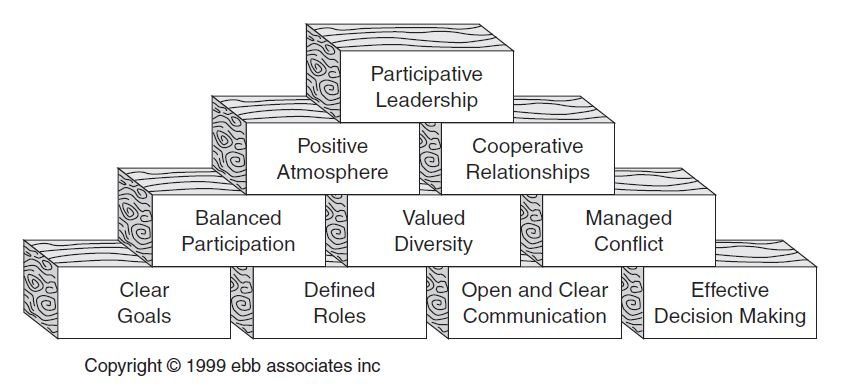
\includegraphics[width=\textwidth]{Abbildungen/Ten_Characteristics.JPG}
%			\caption[Abbildung 1]{Ten Characteristics of a High Performance Team \citep[p. 27]{biech2007pfeiffer}}
%			\label{ten_characteristics}
%		\end{footnotesize}
%	\end{figure}
%	Die einzelnen Teilbereiche bauen aufeinander auf. Der untere Teilbereich mit den Komponenten \textit{Clear Goals"}, \textit{Defined Roles}, \textit{Open and Clear Communication} sowie \textit{Effective Decision Making} sind die Basis des gesamten Models. Diese Komponenten sollten am Anfang des Teambuildingprozesses definiert und immer als Basis der gesamten Teamarbeit gesehen werden.\\
%	Der Teilbereich mit den Komponenten \textit{Balanced Participation}, \textit{Valued Diversity} und \textit{Managed Conflict} baut auf diese auf.\\
%	\textit{Positive Atmosphere} und \textit{Cooperative Relationships} ist der dritte Teilbereich. In diesem geht es hauptsächlich um die Zufriedenheit und die Bereicherung eines einzelnen in einem Team zu arbeiten. Jedoch ist dieser Bereich nicht mehr Ausschlaggebend um eine Aufgabe zu erledigen. Für viele Teammitglieder ist dieser Teilbereich jedoch wichtigste Ziel während der Teamarbeit.\\
%	\textit{Participative Leadership} ist der einzige Bereich der aus dem Gesamtgebilde ohne Beeinflussung der anderen Komponenten entfernt werden kann. Dies sagt uns, dass ein Teamm auch ohne einen einzelnen Teamleiter existieren kann. Vgl. \citep[p. 13-16]{biech2007pfeiffer}\\
%	Aufgrund der vielen Komponenten die ein Team erfüllen muss um effizient zu sein und ein Gestärktes Teamgefühl zu bilden, wird in dieser Ausarbeitung nur auf einen Teilbereich eingegangen.
%	
%			\paragraph{Positive Atmosphere}
%	Wird der Aufbau von Vertrauen vernachlässigt, so bildet sich kein gut funktionierendes Team.
%			\paragraph{Open and Clear Communication}
%			\paragraph{Balanced Participation}
%			\paragraph{Defined Roles}
%	
%		\subsubsection{Team-Colloboraton}
%		\subsubsection{Virtual-Teambuilding}
		
%			\paragraph{Allgemeines}

%EINGEFÜGT BEI DEFINITION EINES VIRTUELLEM TEAMS
%		Virtuelle Teams werden häufig gebildet um räumliche oder kurzzeitige Trennungen eines Teams zu umgehen. Dabei werden computergestützte Technologien so verwendet, dass räumlich getrennte Teammitglieder ihre Aufgaben, mittels computergestützter Kommunikation, im Team koordinieren können. \citep[p. 117-119]{peters2007identifying} \citep[p. 1-2]{cascio2003leadership}
%		
%		Es kann effizient Länderübergreifend gearbeitet werden, was ein größeres Innovationspotential für Unternehmen zur folge hat.	
%		Virtuelle Teams haben den Ruf teuer zu sein, die Ziele nicht verfolgen zu können, nie pünktlich und schwierig zu managen zu sein. \citep[p.243-244]{gassmann2003trends}
%		
%		Virtuelle Teams sind häufig gerade in der Anfangsphase sehr Ergebnisorientiert in der Art und Weise \textit{wie} kommuniziert wird. Dieses Defizit in der Sozialen Kommunikation untereinander kann die Schlüsselfaktoren eines Erfolgreichen Teams beeinträchtigen - Soziale und Emotionale Beziehungsbildung sowie den Aufbau von Vertrauen. \citep[p.378]{ren2007applying} \\
%		Um die Wahrscheinlichkeit zu erhöhen, dass auch in der Anfangsphase des Teambuildings eine \glqq Soziale\grqq und keine \glqq Arbeitsnahe, Ergebnisorientierte\grqq Kommunikation stattfindet, wurde eine spielerische Umgebung geschaffen, in der sich das Team das erste mal kennenlernen kann. 
%		
%Virtuelle Teams werden in dieser Arbeit als temporär, divers und räumlich gerennt, beschrieben. Die Kommunikation untereinander nur durch das World-Wide-Web statt. Weiterhin impliziert die temporäre Eigenschaft der Definition, dass sich die Teammitglieder nicht kennen.
		
		
%		\subsubsection{Einflussfaktoren im Teambuilding}


%	Z.b. Aussehen, Kulturen, etc.	
\newpage
\section{Versuchshypothesen}
\label{Versuchshypothesen}
Aufgrund der vorherig genannten Forschungen, wurden folgende Hypothesen definiert :
\begin{itemize}
	\item{\underline{Hyothese 1} :\\ 
	H1$_{0}$ : Ein hoher General-Trust-Score (\ac{gt}) wirkt sich \textbf{nicht positiv} auf den Cognitiven-Trust-Score (\ac{ct}) aus. \\
	H1$_{1}$ :Ein hoher General-Trust-Score (\ac{gt}) wirkt sich \textbf{positiv} auf den Cognitiven-Trust-Score (\ac{ct}) aus.}
	
Es wird davon ausgegangen, dass Personen, die leicht einen Vertrauensvorschuss gewähren, nicht immer gleichzeitig auch in die Fähigkeiten oder in die Zuverlässigkeiten des Teams glauben.

\item{\underline{Hyothese 2} :\\ 
	H2$_{0}$ : Die Konditionen \ac{ik} oder \ac{nik} haben \textbf{keinen Signifikant abweichenden Einfluss} auf den Cognitive-Trust-Score (\ac{ct}). \\
	H2$_{1}$ : Die Konditionen \ac{ik} oder \ac{nik} haben \textbf{einen Signifikant abweichenden Einfluss} auf den Cognitive-Trust-Score (\ac{ct}).}

%	\item{\underline{Hyothese 2} :\\ H$_{0}$ : Ein Torso, Head und Hand getrackter Avatar (IK) hat \textbf{keinen Einfluss} auf den Cognitiven-Trust-Score.\newline
%	H$_{1}$ : Ein Torso, Head und Hand getrackter Avatar hat \textbf{einen Einfluss} auf den Cognitiven-Trust-Score.}
	
Hat nun ein Head und Hand getrackter Avatar einen Einfluss auf die wahrgenommen Fähigkeiten oder die wahrgenommene Zuverlässigkeit in das Team? Genau diese Frage stellt sich diese Hypothese 2.
Es wird davon ausgegangen, dass, egal welche Kondition des Avatars ein Probant zur Verfügung gestellt bekommt, dies keinen Einfluss auf die wahrgenommenen Fähigkeiten des Teams hat. Somit erscheint ein Team in seiner Leistungsfähigkeit und Zuverlässigkeit immer gleich, egal ob ein Avatar Menschenähnlich ist oder nicht.

	\item{\underline{Hyothese 3} :\\ 
	H3$_{0}$ : Ein hoher Cognitiver-Trust-Score im Team (\ac{teamCogIK} und \ac{teamCogNIK}) hat \textbf{keinen Einfluss} auf die auf die Anzahl der erfolgreich abgeschlossenen Runden (\ac{tRound}) bei unterschiedlichen Avatarverkörperungen (\ac{tRoundIK} und \ac{tRoundNIK}). \\
	H3$_{1}$ : Ein hoher Cognitiver-Trust-Score im Team (\ac{teamCogIK} und \ac{teamCogNIK}) hat \textbf{Einfluss} auf die auf die Anzahl der erfolgreich abgeschlossenen Runden (\ac{tRound}) bei unterschiedlichen Avatarverkörperungen (\ac{tRoundIK} und \ac{tRoundNIK}).}
	
Es wird davon ausgegangen, dass wenn Personen oder Teams sich untereinander Leistungsfähig oder Zuverlässiger ansehen, dies keinen Einfluss auf die Team-Effektivität hat. 
	
	\item{\underline{Hyothese 4} :\\ 
	H4$_{0}$ : Die Konditionen \ac{ik} oder \ac{nik} haben \textbf{keinen Signifikant abweichenden Einfluss} auf die Anzahl der erfolgreich abgeschlossenen Runden \ac{tRound} eines Teams.\newline
	H4$_{1}$ : Die Konditionen \ac{ik} oder \ac{nik} haben \textbf{einen Signifikant abweichenden Einfluss} auf die Anzahl der erfolgreich abgeschlossenen Runden \ac{tRound}}
	
%	\item{\underline{Hyothese 4} :\\ H$_{0}$ : Ein Torso, Head und Hand getrackter Avatar hat \textbf{keinen Einfluss} auf die Team-Effektivität. \newline
%	H$_{1}$ : Ein Torso, Head und Hand getrackter Avatar hat \textbf{Einfluss} auf die Team-Effektivität.}	
	
In dieser Hypothese wird sich mit der Frage beschäftigt, ob ein Team effektiver (mehr Runden abschließt) ist, je nachdem welche Avatar Kondition diesem zugeordnet wird. Es wird davon ausgegangen, dass die Team-Effektivität nicht aufgrund der Menschenähnlichkeit variiert.

	\item{\underline{Hyothese 5} :\\ 
	H5$_{0}$ : Teams, aufgeteilt nach Avatarverkörperungen (\ac{ik}, \ac{nik}), mit einem hohem General-Trust-Score (\ac{gt}) erzielen \textbf{keine höhere Team-Effektivität} (\ac{tRound} als die mit einem niedrigen General-Trust-Score \ac{gt}. \newline
	H5$_{1}$ :  Teams, aufgeteilt nach Avatarverkörperungen (\ac{ik}, \ac{nik}), mit einem hohem General-Trust-Score (\ac{gt}) erzielen \textbf{eine höhere Team-Effektivität} (\ac{tRound}) als die mit einem niedrigen General-Trust-Score \ac{gt}}.
\end{itemize}

Sind eventuell Teams in der \ac{vr} Effektiver, nur weil diese generell leichter einen Vertrauensvorschuss gewähren? Genau dieser Frage geht Hypothese 5 nach. Es wird jedoch davon ausgegangen, dass Teams keine höhere Teameffektivität erzielen, auch wenn diese einen höheren Hang zum Vertrauen haben.

%\textbf{NEU}
%
%\begin{itemize}
%	\item{H1 : Probanten mit einem hohen General-Trust-Score erzielen auch einen hohen Cognitiven-Trust-Score.}
%	\item{H2 : Probanten, die einen Torso, Head und Hand getrackter Avatar nutzen erzielen einen höheren Cognitiven-Trust-Score.}
%	\item{H3 : Ein hoher Cognitiver-Trust-Score wirkt sich positiv auf die Team-Effektivität aus.}
%	\item{H4 : Ein Torso, Head und Hand getrackter Avatar hat einen positiven Einfluss auf die Team-Effektivität.}
%	\item{H5 : Teams, mit einem generell hohem Hang zum Vertrauen erzielen auch eine hohere Team-Effektivität.}
%\end{itemize}


Diese wurden in einer Grafik Veranschaulicht um einen besseren Gesamtüberblick zu erhalten.

\begin{figure}[H]
		\begin{footnotesize}
			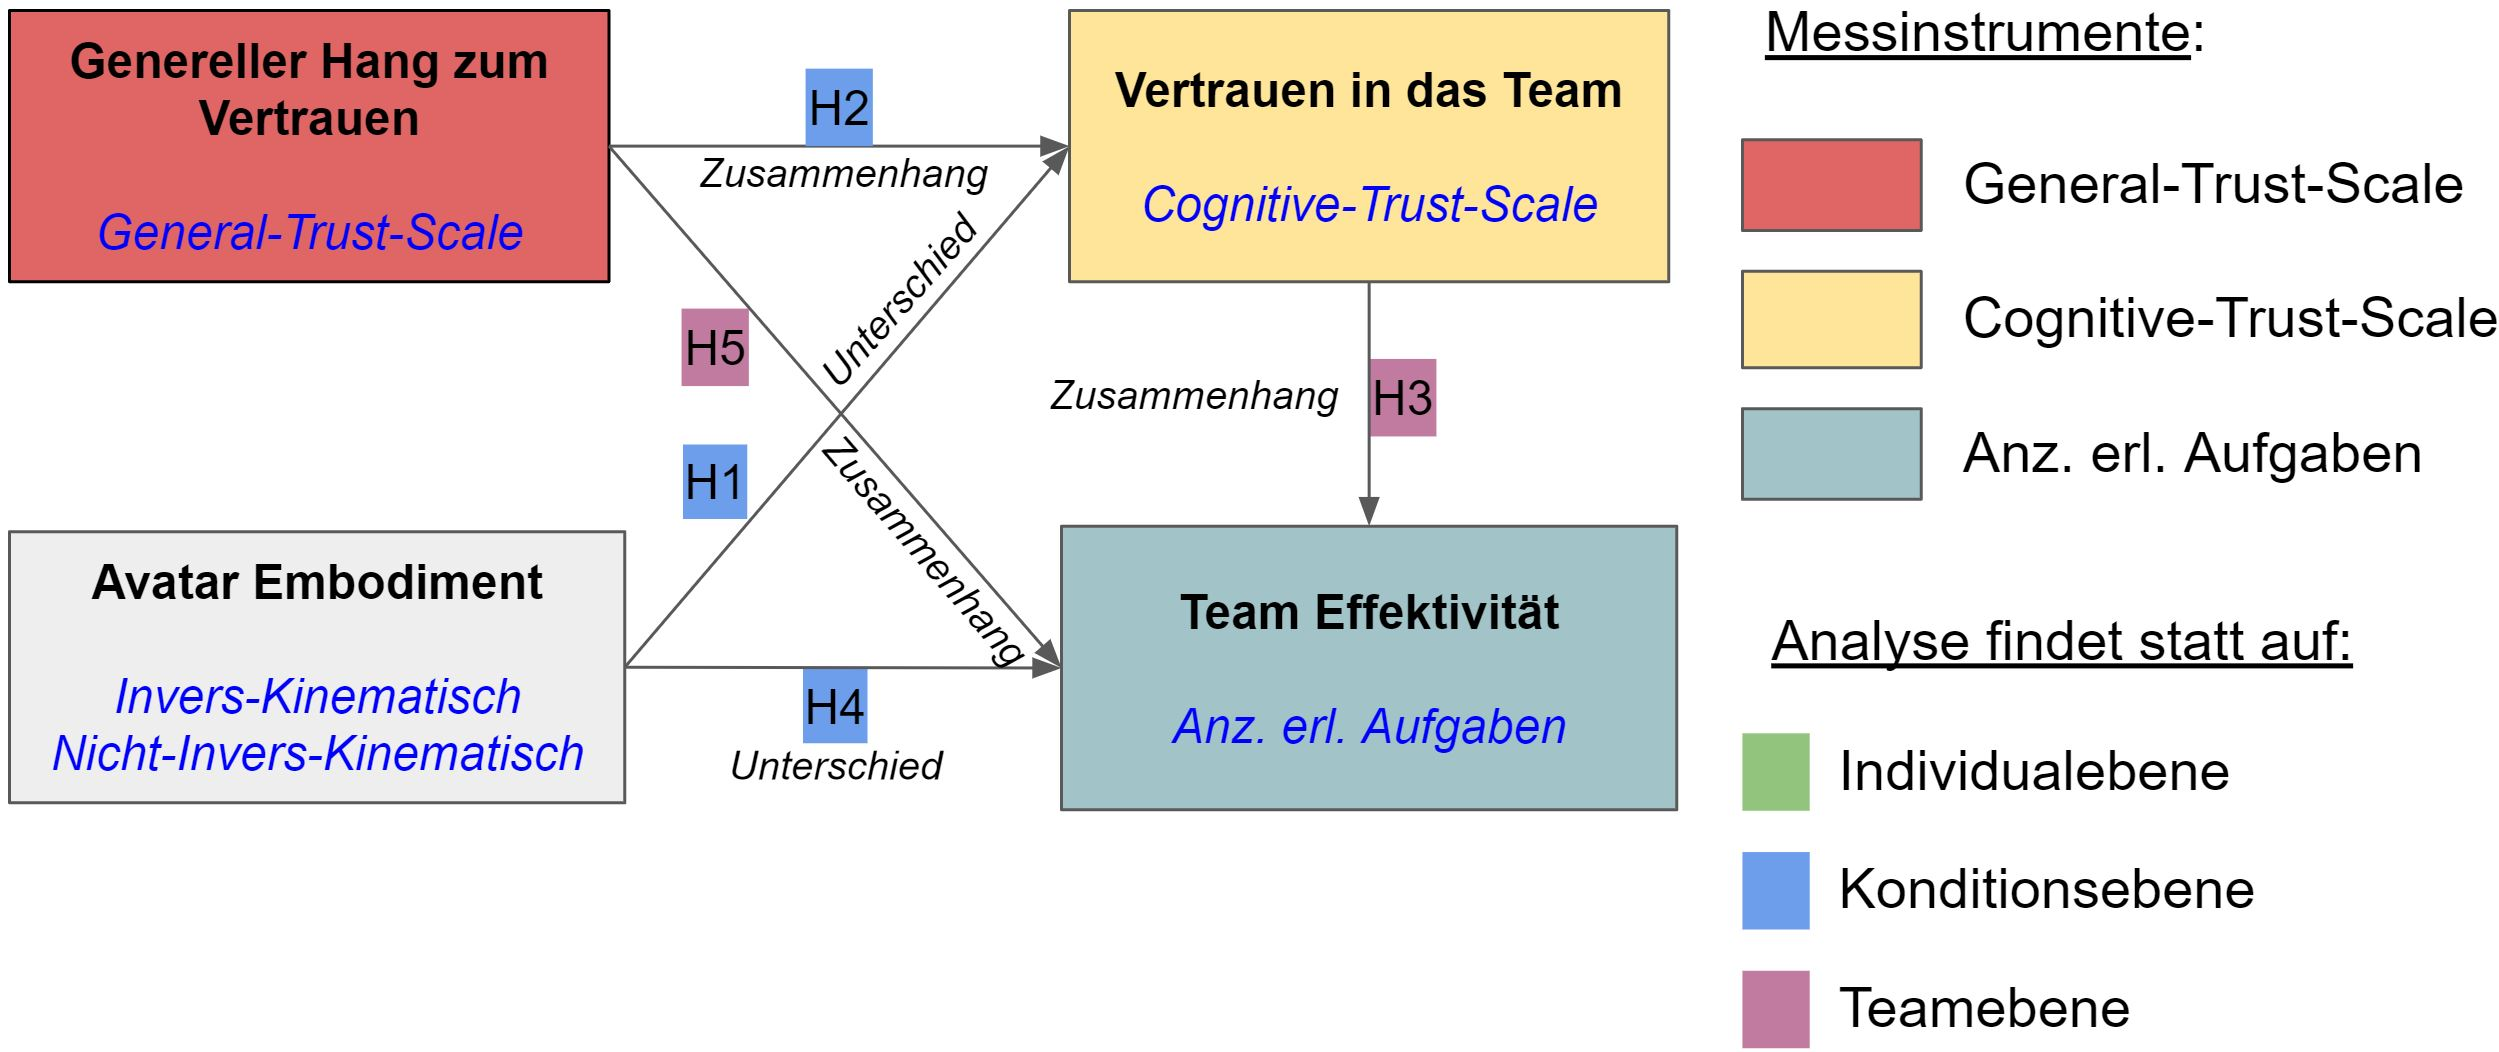
\includegraphics[width=\textwidth]{Abbildungen/Versuchshypothesen_02.JPG}\\
			\caption{Versuchshypothesen}
			\label{Versuchshypothesen}
		\end{footnotesize}
	\end{figure}	

\newpage
	\section{Vorgehensweise}
	\subsection{Der Versuch}
	\subsubsection{Beschreibung des Forschungsverlaufs}
Insgesamt nahmen 30 Teilnehmer an dem Versuch Teil. Da ein Team aus 3 Teilnehmern bestand, waren es insgesamt 10 Teams. Jedes Team bekam entweder die Kondition \ac{ik} oder \ac{nik} zugeordnet. Somit gab es 5 \ac{ik} sowie 5 \ac{nik} Teams.
Jeder Probant bekam einen zufälligen Zeitslot sowie ein anonymen Namen zugeordnet mit dem dieser an dem Versuch teilnahm. Gemäß des A/B-Testings wurden jeweils drei Personen in einem Zeitslot untergebracht um ein "Team" zu bilden. Diesem "Team" wurde entweder die Kondition \ac{ik} oder \ac{nik} zugeordnet. Somit nahmen drei Probanten, an einem Versuch zur selben Zeit mit der selben Kondition, teil. Die Probanten wurden nicht Face-To-Face vorgestellt und sahen sich während des gesamten Versuchs nur als Repräsentation eines Avatars in dem \ac{sve}. Der Zeitslot von 30 Minuten teilte sich auf in
		\begin{itemize}
			\item 5 Minuten Pre-Questionnaire
			\item 5 Minuten Videoerklärung
			\item 15 Minuten Versuchsdurchführung
			\item 15 Minuten Post-Questionnaire
		\end{itemize}
Jeder Teilnehmer bekam zu beginn seines Zeitslots einen Pre-Questionnaire ausgehändigt, den dieser selbstständig ausfüllen sollte. In diesem wurden Fragen über die \dq{}Person\dq{}, über eventuelle \dq{}Gesundheitliche Beschwerden\dq{} sowie schon vorhandene \dq{}\ac{vr}-Erfahrung\dq{}, gestellt.
Dieser wurde von 30 Personen ausgefüllt.
Alle Probanten mussten sich anschließend ein Video über die Erklärung des Experiments anschauen. So wurde sichergestellt, dass alle Probanten den Selben Informationsgehalt über die Art und Weise des Ablaufs des Experiments bekamen. Alle Mitglieder eines Teams starteten somit mit den selben Informationen.
Nachdem alle Probanten die Videoerklärung angeschaut hatten, begann das Experiment. Dazu loggte sich das jeweilige Team in das \ac{sve} ein und spielten den Versuch durch.
		Am Ende der Versuchsdurchführung, wurde ein Post-Questionnaire ausgeteilt. In diesem wurden Fragen über das \dq{}Generelles Vertrauen\dq{}, das \dq{}Kognitive Vertrauen\dq{} die \dq{}Kommunikations-Qualität\dq{}, die wahrgenommene \dq{}Team-Effektivität\dq{}, die \dq{}Beanspruchung\dq{} sowie die \dq{}Presence\dq{}, gestellt. Am Ende war es jeden Teilnehmer zusätzlich möglich ein Feedback zu geben. Der Post-Questionnaire wurde von 30 Personen ausgefüllt. 
		
Die maximale Versuchsdauer nach Start der Anwendung betrug exakt 10 Minuten (600 Sekunden). Es konnten maximal 15 Runden absolviert werden, wobei jede Runde inkrementell schwieriger wurde, da jede 3. Runde jeweils 1 Symbol, in den Pool der zu erratenden Symbole, hinzukam. 

	\subsubsection{Allgemeiner Versuchsaufbau}

\begin{figure}[H]
		\begin{footnotesize}
			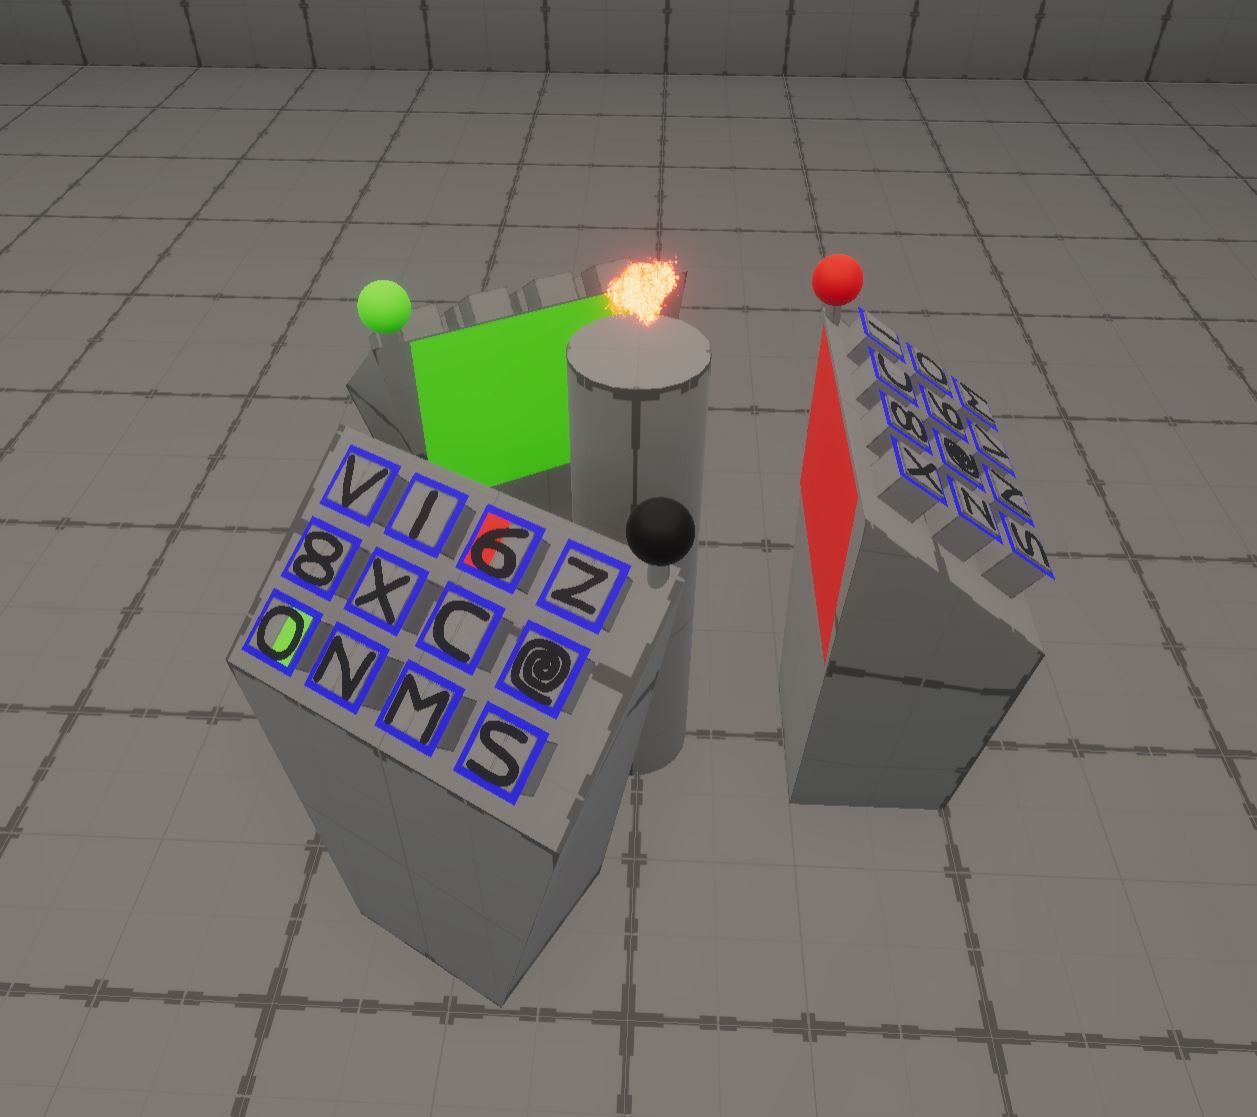
\includegraphics[width=\textwidth]{Abbildungen/Podeste.JPG}\\
			\caption[Abbildung 1]{Die Podeste der Teilnehmer}
			\label{Framework}
		\end{footnotesize}
	\end{figure}

Jeder Probant benötigte (neben einem funktionsfähigen Computer), um an dem Versuch teilnehmen zu können, entweder ein Oculus, HTC-Vive oder Windows Mixed-Reality\ac{hmd}, sowie zwei funktionsfähige Controller.

Dem Versuchsleiter war es während der gesamten Anwendung möglich, die 3 Probanten durch einen eigenen Client zu betreuen. Alle Probanten konnten durch Ihre Anwendung durch das integrierte Mikrofon im \ac{hmd} zu dem Versuchsleiter Sprechen und diesen hören. Während die Probanten sprachen, konnten die anderen zwei Probanten diese jedoch nicht hören. Die Sprachkommunikation eines Probanten war somit nur Richtung Versuchsleiter möglich. Dies dient zur Vermeidung von einigen Störvariablen und zum Erhalt der Integrität der Anonymität.
Während der Versuchsleiter sprach, konnten jedoch alle Probanten den Versuchsleiter hören. Dies diente dazu, eventuelle offene Fragen an alle Versuchsteilnehmer weiterzugeben und den Beginn sowie das Ende der Anwendung zu kommunizieren. Der Versuchsleiter gab jedoch während des gesamten Versuchs keine Hilfestellung.

In der Anwendung war es den Probanten möglich mittels der Tasten \dq{}W A S und D\dq{} ihre Position und mittels den Tasten \dq{}Q\dq{} und \dq{}E\dq{} ihre Höhe, in einem gewissen Bereich, zu ändern. Dies stellte sicher, dass alle Probanten ihre Avatargröße und Position individuell an ihre Körpergröße anpassen konnten.

Da es den Probanten nicht möglich sein sollte, auf die Symbole der anderen teilnehmenden Probanten zu schauen, wurde ab einer gewissen Grenze Links und Rechts des Podest der Probanten ein \dq{}Fade-To-Black\dq{} Mechanismus eingebaut. Kamen die Probanten mit dem Kopf ihres Avatars in diesen Bereich, sahen diese nur noch die Farbe Schwarz und mussten sich zurückbewegen.

Waren alle Probanten bereit, wurden diese vor ein für Sie eigenes Podest teleportiert und sahen einen Countdown zwischen den 3 Podesten herunter zählen. Dieser Countdown litt den baldigen beginn einer Runde ein.
Wurde eine Runde gestartet, wurde das Podest jedes Probanten eineindeutig durch die Farbe \dq{}Schwarz, Rot oder Grün\dq{} markiert. Die Probanten konnten Ihre und die Farbe des Spielers an einem Viereck sowie einer runden Kugel in der jeweils zugeteilten Farbe, an den jeweiligen Podesten, erkennen. Die Farbe der einzelnen Probanten änderte sich jede Runde.

	\subsubsection{Detaillierter Versuchsablauf}

Der Schwarz markierte Probant war mit dem Erklären in der jeweiligen Runde an der Reihe.
Auf dem jeweiligen Podest eines Probant befanden sich verschiedene Symbole. Diese Symbole waren für alle Probanten gleich, jedoch an unterschiedlichen Positionen. Der Schwarz markierte Probant hatte an den Symbolen noch entweder die Farbe \dq{}Grün oder Rot\dq{} oder \dq{}Grün und Rot\dq{}.
Der schwarz markierte Probant versuchte nun, mittels Hand und Armbewegung, den Rot und Grün markierten Probant die Symbole, die in der jeweiligen Spielerfarbe vor Ihm markiert waren, zu erklären.
Meinte ein Probant (Rot oder Grün), dem der schwarz markierte Probant ein Symbol erklärt hat, ein Symbol erkannt zu haben, loggte dieser das Symbol durch herunterdrücken des Knopfes an seinem Podest, mit dem jeweiligen erkanntem Symbol, ein. Der Schwarz markierte Probant musste nichts einloggen oder klicken, sondern nur durch Gestikulation erklären.
Hat ein Probant sich während des einloggens verklickt oder wollte seine Meinung zum erkanntem Symbol ändern, musste das Symbol vorher, durch erneutes klicken des Symbols vor ihm, ausgeloggt werden. Anschließend konnte es erneut eingeloggt werden.
Wurden alle Symbole vom roten und grünem Probant erkannt und eingeloggt, die der schwarz markierte Probant angezeigt hat, wurde dies durch eine grüne Kugel, für alle Sichtbar, erkennbar gemacht und die Runde endete. Erschien diese grüne Kugel nicht, war noch etwas falsch und der schwarz markierte Probant musste noch einmal versuchen die korrekten Symbole den jeweiligen Mitspielern aufzuzeigen.
In der nächsten Runde wurde ein anderer Probant eineindeutig mit Schwarz, Rot oder Grün markiert.
Mit steigender Anzahl an erfolgreich bestandenen Runden, müssen mehr Symbole erfolgreich erkannt werden.

Das Ziel war es nun, so viele Symbole wie möglich gemeinsam korrekt zu bearbeiten und dadurch in höhere Runden aufzusteigen.

	\subsubsection{Die Avatare}
Die Avatare im \ac{sve} wurden als \dq{}IK-Avatar\dq{} und \dq{}Non-IK-Avatar\dq{} implementiert.
Für beide Avatararten wurde die neutrale Farbe Schwarz gewählt. Die Probanten hatten keinen Einfluss auf die Farbwahl ihres eigenen Avatars. Dies dient dazu die Störvariable der eventuell vorhandenen Vorurteile des Mitspielers aufgrund der Farbe des Avatars, auszuschalten. Je nach Kondition \dq{}IK-Avatar\dq{} oder \dq{}Non-IK-Avatar\dq{} bekam jeder Probant das Selbe aussehen des Avatars zugeordnet. Der eigene Avatar ist nicht für die Mitspieler sichtbar. Zur besseren Interaktion mit den Knöpfen sowie zur höheren Immersion, wurde der eigene Avatar nicht sichtbar für den Probanten dargestellt. Jeder Probant, unabhängig der zugewiesenen Kondition sah somit nur eine Repräsentation von menschlich wirkenden Händen.

	\begin{figure}[H]
		\begin{footnotesize}
			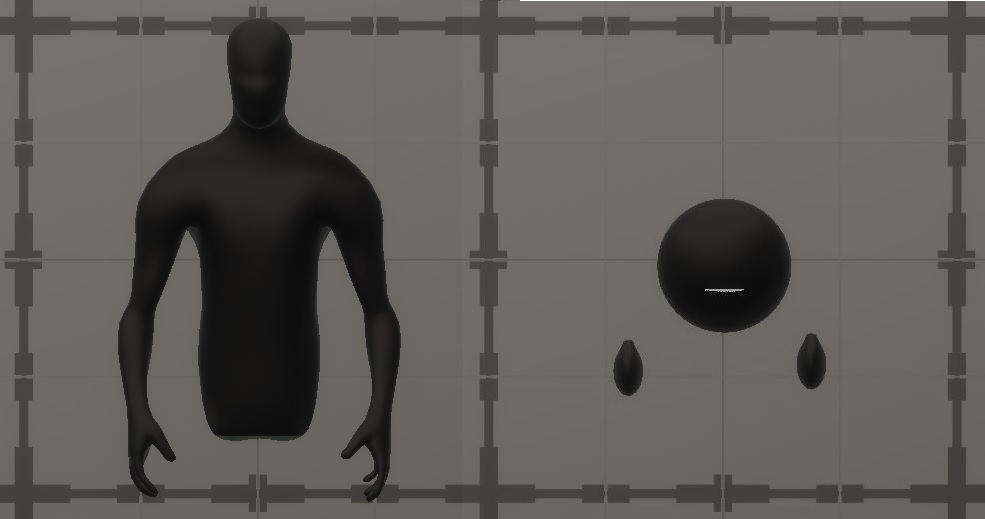
\includegraphics[width=\textwidth]{Abbildungen/Avatars.JPG}\\
			\caption[Abbildung 1]{Links: IK-Avatar, Rechts: Non-IK-Avatar}
			\label{Framework}
		\end{footnotesize}
	\end{figure}

		\paragraph{IK-Avatar}
Der Invers-Kinematisch getrackte Avatar hat ein Androgynes aussehen, um die Störvariable rund um Vorurteile aufgrund des Geschlechts der Probanten auszublenden. Der IK-Avatar besitzt keine Augen, Mund, Haare oder Beine, lediglich einen Oberkörper mit Kopf.
Um eine Möglichst realistische Bewegung zu erzielen, wurde die Handbewegung, die Unterarmbewegung, die Oberarmbewegung sowie die Kopf-und Torsorotation simuliert.

		\paragraph{Non-IK-Avatar}
Der Non-IK-Avatar besteht aus einem Kreis mit Mund sowie einer Repräsentation der Linken sowie der Rechten Hand. Er Besitzt keine Augen, Haare, Beine, Hals, Torso sowie Ober- und Unterarm. Der Mund dieses Avatars ist als unauffälliger Orientierungspunkt des Kopfes erhalten geblieben. Der Mund des Non-IK-Avatars bewegt sich jedoch nicht. 
	\newpage

	\subsection{Entwicklung der Versuchsumgebung}
Um den Versuch durchzuführen, wurde ein \ac{sve} entwickelt in dem Sich die 3 Teammitglieder gegenseitig Sehen und miteinander interagieren konnten. 
Das \ac{sve} wurde mit Unity 2019.4.3f1 und der HD-Render-Pipeline programmiert. Um die Echtzeitkommunikation zwischen den einzelnen Clients zu gewährleisten, wurde das multiplayer Framework \dq{}Normcore v2.0\dq{} \footnote{www.Normcore.io} genutzt.
Normcore unterstützt Network-Physics, automatische Realtime-Synchronisation, Voice-Chat, XR-Compitabilität sowie persistente multiplayer Räume.	

\paragraph{Normcore Datastore / Sync Mechanismus}
Normcore besitzt das konzept eines globalen Datastore.  Alle Zustände, egal ob die Position eines Spielers, einzelne bool, integer oder float Variablen, werden in einem globalen Datastore gespeichert. Werden Objekte in der Anwendung bewegt, synchronisiert Normcore diese Änderung der Position und/oder Rotation mit allen anderen Mitspielern automatisch.

\paragraph{Verwendete Hardware}
Um an dem Experiment Teilnehmen zu können, benötigten die Probanten ein im vollem Umfang funktionierendes HTC-Vive, HTC-Vive2 oder ein Oculus-Rift S \ac{hmd} mit funktionsfähigen Controllern sowie einen Leistungsstarken \ac{vr}-Fähigen PC. Der Spectator, der das Experiment Remote steuern und verwaltet, benötigt einen Leistungsstarken PC auf dem die Anwendung ausführbar ist.

\paragraph{Aussehen der Umgebung}
Der Raum, in dem die Spieler sich befinden ist ein Rechteckiger Raum mit 4 Fenstern vor denen einige Low-Poly Bäume stehen. Durch die 4 Fenster und den davor plazierten Bäumen sollte eine gewisse Offenheit erzeugt werden, damit die Probanten sich nicht in der \ac{vr} eingeschlossen fühlten. Weiterhin wurde der Raum schlicht in einer gräulichen Farbe gehalten um  nicht all zu viel Ablenkung in der \ac{vr} zu erzeugen. Die Spieler sollten sich so gut es geht nur auf den eigentlichen Versuch konzentrieren. 

\paragraph{Raumerschaffung in Normcore}

\paragraph{Spectator und Client}

\paragraph{VR-Client}
Jeder Versuchsteilnehmer benötigt eine Client Version der Umgebung um an dem Versuch teilzunehmen. Die Client Version gibt es in drei verschiedenen Versionen. Diese verschiedene Versionen unterstützen die HTC-Vive \ac{hmd}'s, die Oculus Rift \ac{hmd}'s sowie die Windows Mixed-Reality \ac{hmd}'s. Beim Start des Clients gelangt der Probant in das \ac{sve} und verbindet sich automatisch mit dem Server (Normcore-Raum).
Der Client sieht seine beiden Hände, jedoch keine der beiden Avatarkonditionen \ac{ik} oder \ac{nik}, sondern menschenähnliche Hände.

\paragraph{Spectator}
Der Spectator besitzt ein eigenen Client, dieser eigene Client hat keine eigene Repräsentation des Körpers und benötigt daher auch kein \ac{hmd} um an der Session teilzunehmen. Dem Spectator ist es möglich sich frei mit der Kamera in der Umgebung zu bewegen.
Der Spectator besitzt die Möglichkeit das Spiel zu starten, die Nummer der zu beginnenden Runde einzustellen, einen Restart durchzuführen, die verbundenen Spieler anzuzeigen und herauszuwerfen, die Avatarkondition der Clients zwischen \ac{ik} und \ac{nik} zu wechseln sowie das Spiel zu verlassen.
Je nachdem, wie viele Spieler in dem entsprechendem Raum sind, werden diese dem Spectator angezeigt. So sieht der Spectator "Player 1" bis "Player 3" bei einem vollem Team auf seinem Bildschirm. Der Spectator besitzt außerdem die Möglichkeit Spieler herauszuwerfen, um die Session aufzuräumen und für die nächsten Teams vorzubereiten.
Weiterhin besitzt der Spectator noch einige Funktionen um sich Informationen über das aktuelle Spielgeschehen zu machen. So bekommt dieser die gesamte vergangene Zeit angezeigt, in welcher Runde sich die Mitspieler aktuell befinden, die aktuelle Effizienz des Teams, ob der "Grüne" oder "Rote" Spieler aktuell mit ihrer Eingabe korrekt sind und wie viele verschiedene Symbole der "Schwarze" Spieler aktuell erklären muss.

\paragraph{Rundenschwierigkeit}
Ein Scriptable Object namens "RoundRules" beinhaltet die Regeln sowie den Ablauf der einzelnen Runden. 
Durch diese Sammlung von Regeln und Abläufen, bekommt jedes Team jeweils in der selben Reihenfolge die selben Zeichen angezeigt um Konsistenz zu gewährleisten. Es beinhaltet somit die allgemeinen "Rundeneinstellungen" des Spiels. Es gibt vor, in welcher Runde die Spieler wie viele Symbole zu erklären und zu erraten haben, welche Knöpfe mit Symbolen gedrückt werden müssen und wer der Schwarze, Rote und Grüne Spieler der jeweiligen Runde ist. Die Regeln wurden so definiert, dass der erklärende Spieler spätestens jede 3. Runde wieder mit dem erklären an der Reihe ist. Die anderen Runden ist dieser der erratende Spieler. Jede 3. Runde wird die Anzahl der zu erratenden und dadurch auch der zu erklärenden Symbole um 1. erhöht. Somit mussten in Runde 1-3 1 Symbol, 4-6 2 Symbole, 7-9 3 Symbole, 10-12 4 Symbole und Runde 13-15 5 Symbole erraten und erklärt werden.
Wer zu welcher Runde der Schwarze, Grüne oder Rote Spieler ist, und welche Symbole welche Runde gedrückt werden mussten, wurde einmalig Pseudozufällig festgelegt und in den "RoundRules" festgelegt.

\paragraph{Avatarkonditionen}
Betritt ein Versuchsteilnehmer das \ac{sve}, bekommt dieser als Selbstrepräsentation seine eigenen, menschenähnlichen Hände zu sehen. Die Versuchsteilnehmer sehen nicht ihre eigene Repräsentation der Konditionen \ac{ik} oder \ac{nik}. Es wird nur die jeweilige Avatarkondition der Mitspieler gesehen.
Falls schon ein anderer Spieler im \ac{sve} anwesend ist oder zu einem späterem Zeitpunkt hinzukommt, ist dieser als die vom Spectator jeweilig ausgewählte Avatarkondition zu sehen. 

\paragraph{GameManager und PodestManager}
Der GameManager übernimmt alle wichtigen Funktionalitäten in der Anwendung.
Diese sind unter anderem :
\begin{itemize}
\item Steuerung und Entscheidungslogik über Spectator oder Spieler
\item Auswahl des Entsprechenden \ac{hmd}'s
\item Netzwerkmanagement und RPC Handling
\item Start, Reset, Steuerung und Überprüfungsmechanismen sowie Zeitmessungen der einzelnen Runden
\item Interaktionen mit globalen Datastore-Variablen
\item Verwalten der CSV-Logs
\end{itemize}

Die Hauptaufgabe des GameManagers ist die gesamte Verwaltung der Anwendung. Der GameManager des Spectator sowie des Clients besitzt unterschiedlichen Funktionalitäten. 
Der GameManager des Clients übernimmt das für den Clienten relevante RPC-basierte Netzwerkhandling sowie das lauschen auf Änderungen von relevanten Variablen im globalen Datastore.
Eine wesentliche Aufgabe ist es zu überprüfen, ob eine Runde vom GameManager des Spectators als beendet markiert wurde und leitet gegebenenfalls die Initialisierung einer neuen Runde ein.
Der GameManager des Spectators gibt Hauptsächlich die Information über den Start, Stop oder den Reset der einzelnen Runden an die GameManager der Clients weiter. Weiterhin steuert dieser aufgrund seiner besonderen Rolle noch die Spectator-to-Client Netzwerkinteraktionen wie die Audioübertragung, Kickmechanismen, Rundenauswahl sowie das Aussehen der Avatare der Spieler.

Jeder Client besitzt einen GameManager. Dieser steht in Verbindung mit den einzelnen Podesten der Spielers. Der Podestmanager eines jeweiligen Clients verwaltet einzelne Podeste, welche wiederum die einzelnen Knöpfe auf den Podesten verwalten. 
Drückt nun ein Spieler ein entsprechenden Knopf mit einem Symbol, sendet der Knopf eine Information über seinen Zustand an den Podestmanager des Clients. Dieser Überprüft wiederum, ob die zur Zeit gedrückten Knöpfe mit den zu drückenden Knöpfen der Runde übereinstimmen. Falls die gedrückten Knöpfe die richtigen sind, wird eine boolean-Variable in einem globalen Datastore umgeschaltet, der den GameManager des Spectators darüber informiert, dass ein Teilnehmer die korrekten Knöpfe gedrückt hat. Haben nun beide Spieler \dq{}Rot und Grün\dq{} die korrekten Knöpfe gedrückt und dadurch eine Flag im globalen Datastore über die jeweilige Korrektheit gesetzt, registriert der GameManager des Spectators dies und setzt ein Flag über das Erfolgreiche abschließen der Runde. Die Clients registrieren dies und leiten die Startsequenz der nächsten Runde ein. 

\paragraph{Audioübertragung}
Die Audioübertragung wird von den GameManagern des Clients sowie des Spectators übernommen. Sobald der Teilnehmer zu der Anwendung verbunden ist, wird das Mikrofon des \ac{hmd}'s aktiviert. Es werden unterschiedliche MessageID's für Spectator und Client für die Netzwerkpakete festgelegt. Die serialisierten Audiodaten werden mittels RPCMessage an alle verbundenen Teilnehmer gesendet. Der Spectator ließt nur die Netzwerknachrichten mit der MessageID der Clients und der Client ließt nur die Netzwerknachrichten mit der MessageID des Spectators.
\newpage
\paragraph{Fade-to-Black und Positionsmanagement}
	Da alle Mitspieler sich in dem \ac{sve} frei bewegen können, müssen diese beim Start des Spiels vor ein Podest platziert werden. Startet der Spectator das Spiel, überprüft ein im globalen Datenspeicher liegendes Byte, wobei die Bits des Bytes als Boolean genutzt wurden, welche Podeste noch nicht belegt sind. Alle Mitspieler werden dementsprechend auf die freien Positionen vor den Podesten teleportiert.
Damit es dem roten sowie dem grünen Spieler nicht einfach möglich ist, auf die markierten Symbole des schwarzen Spielers zu schauen, indem der jeweilige Spieler dort hin läuft, wurde ein Fade-To-Black Mechanismus implementiert. Entfernt sich ein Spieler in einem bestimmten Radius von seinem Podest, wird sein Bild ab diesem Zeitpunkt zunehmend schwärzer, je weiter der Spieler sich entfernt. Die Schwärze verschwindet, desto näher der Spieler sich dem maximal erlaubtem Radius wieder nähert.

\paragraph{CSV-Logwriting}
Der GameManager des Spectator sammelt alle relevanten Daten über die Clients, während die einzelnen Runden von den Teilnehmern durchgeführt werden. Es wird inkrementell ein CSV-Log pro Durchgang fortgeschrieben. Dieses Log umfasst unter anderem das Startdatum, die Startzeit, die Spielzeit, die Rundenzeit, die Rundennummer %einen Effizienzwert berechnet durch $1-\frac{timeSinceGameStarts}{OverallGameTime}$ ( welcher jedoch nicht verwendet wurde ),
sowie welche Avatarkondition in diesen Durchlauf verwendet wurde.

%\paragraph{Physical Handmodel, eigener Avatar war unsichtbar}
%
%\paragraph{PlayerDisconnection Handling, Player Kick Mechanism, Destroying of Network Audio Receiver}
%
%\paragraph{Symbole und Podest, Drückmechanismus, Colliderplatzierung}
%Eingeloggt ist Gelb umrandet etc auch erklären, Ausloggen etc. Depth of button

\paragraph{Gametimer Funktionsweise}
Die jeweiligen Teams haben 600 Sekunden Zeit, um so viele Symbole wie möglich, richtig zu erkennen. Um sich auf die startende Runde vorzubereiten, zählt ein Timer von 10 herunter. Anschließend beginnt die Runde. Dieser Spiele-Timer ist von jedem Mitspieler zwischen den drei Podesten gut sichtbar und immer zu den einzelnen Versuchsteilnehmern hingedreht. Die 10 Sekunden zwischen den einzelnen Runden, werden nicht Gesamtzeit hinzugezählt. Schaffen die Versuchsteilnehmer 10 Runden in 600 Sekunden zu absolvieren, dauert der Versuch somit insgesamt \\
$600 Sekunden Gesamtzeit + 10 Runden * 10 Sekunden Wartezeit = 700 Sekunden$.

\paragraph{PlayerHeight/Position Change}
Die unterschiedlichen Körpergrößen und unterschiedlichen Zimmergrößen der Versuchsteilnehmer müssen berücksichtigt werden.
Falls eine Person zu klein oder zu groß für das Podest ist, kann dieser seine Spielerkamera inklusive Avatar mit den Tasten Q und E bis zu einem bestimmten Schwellenwert höher oder niedriger stellen. Durch diesen Mechanismus ist es auch sitzenden Personen möglich, an dem Versuch teilzunehmen.
Falls der Raum zu klein oder aus anderen Gründen im realem Raum nicht genügend Platz vorhanden ist, um die Knöpfe auf dem Podest zu betätigen, können sich die Spieler mit den Tasten W, A, S und D vorwärts, links, rechts und rückwärts in Blickrichtung bewegen.

\paragraph{Animationen, Shadergraph und VFX-Graph}
Die teilnehmenden Personen können in dem \ac{sve} lediglich virtuelle Hände ihrer eigenen Körperrepräsentation sehen. Da die Hauptinteraktion das Drücken der Knöpfe des zugeteilten Podestes darstellt, soll dies für die teilnehmenden Personen so einfach wie möglich gestaltet sein. Die teilnehmende Person soll sofort verstehen, wie diese mit seinem Avatar einen Knopf drückt. Die virtuellen Hände besitzen das Aussehen echter Hände mit einem grau-hellgrauem Karo-Muster Überzug. Drückt eine teilnehmende Person den Triggerbutton seines Controllers, schließen sich alle Finger zu einer Faust.

Drückt ein Spieler einen Knopf mit Symbolen, bekommt dieser durch eine gelbe Umrandung des Knopfes die Bestätigung, dass dieser den Knopf eingeloggt hat. Drückt dieser diesen erneut, verschwindet die gelbe Umrandung. Diese Umrandungen Leuchten im Ping-Pong-Effekt auf und wurden mit Unity Shader-Graph erstellt.

Ist eine Runde noch nicht abgeschlossen, sehen die Teilnehmer zwischen den Podesten einen leuchtenden Ball, welcher aus Unitys VFX-Graph Partikelsystem besteht. Wird eine Runde beendet, wechselt die Farbe des Partikelsystems von Rot auf Grün und es wirkt eine Kraft im Zentrum des Partikelsystems auf die einzelnen Partikel ein und schleudert diese auseinander.

\paragraph{Sounds}
Ist ein Teilnehmer den Raum beigetreten, wurde ein selbstaufgenommener Sound "Player Connected" abgespielt. Hat ein Disconnect eines Teilnehmers stattgefunden, wurde der Sound "Player Disconnected" abgespielt.
Um ein Feedback bei erfolgreichen Buttonklicks bereitzustellen, wurde ein "Klick" sound beim drücken eines Buttons abgespielt.
Alle Clients konnten mit dem Spectator sprechen. Dieser konnte alle Clients hören und zu allen auf einmal sprechen. Clients konnten keine Clients hören oder zu diesen Sprechen.
\paragraph{UML Diagramme der Funktionsweise}
	
Wirklich?
	
\subsection{Methodik}
\subsubsection{Untersuchungsmethode}
Um die beiden Unabhängigen Variablen \dq{}Non-IK-Avatar\dq{} und \dq{}IK-Avatar\dq{} innerhalb einer Teambuildingmaßnahme zu testen, wurde das A/B-Testing in kombination einer Quantitativen Forschung gewählt.
Gruppe A bekam dabei die Kondition \dq{}Non-IK-Avata\dq{} zugeteilt, während Gruppe B die Konditiion \dq{}IK-Avatar\dq{} zugeteilt bekam. Diese Aufteilung, welcher Probant welche Kondition zugeteilt bekam, erfolgte nach dem Zufallsprinzip. 

	\subsubsection{Teilnehmerfindung}
Da das gesamte Experiment als Into-the-Wild Experiment aufgebaut wurde, wurde in verschiedenen Foren ( z.B. VRForum.de, Computerbase.de, Hardwareluxx.de, etc. ) durch eine Suchanfrage, in Form eines extra dafür angelegten Threads, Teilnehmer gesucht. Weiterhin wurden Teilnehmer durch verschiede Facebookgruppen mit einem Bezug zu \ac{vr}, sowie durch zufällige Whatsapp-Chatgruppen mit 50+ Mitgliedern, akquiriert. Da das gesamte Experiment, sowie die Versuchsanleitung auf deutscher Sprache erstellt wurde, fand die Teilnehmerfindung nur im deutschsprachigem Raum statt.
Die Voraussetzung um an dem Versuch Teilzunehmen, ist es, ein \ac{hmd}, zwei Controller sowie ein Computer mit Internetzugang zu besitzen. Der gesamte Versuch ist als ein "Into the Wild" Versuch aufgebaut, welches bedeutet, dass die genaue Zielgruppe nicht genau definiert werden kann. Die einzigen Ristriktion an die Zielgruppe ist, dass diese die zu verwendete Hardware besitzen.\\
		
	\subsubsection{Unabhängige Variablen}
Als unabhängige Variablen wurden der \dq{}IK-Avatar\dq{} sowie der \dq{}Non-IK-Avatar\dq{} gewählt. Durch diese  unabhängigen Variablen wurde im weiterem Versuchsverlauf versucht den Einfluss auf die abhängigen Variablen zu bestimmen.
Insofern wird untersucht, wie der Einfluss von dem \dq{}IK-Avatar\dq{} sowie dem \dq{}Non-IK-Avatar\dq{} auf das Generelle-Vertrauen, das Vertrauen im Team sowie auf die Team-Effektivität ist.

	\subsection{Abhängige Variablen}
		\subsubsection{Hang zum  Vertrauen}
Der Hang zum Vertrauen bezieht sich in dieser Studie darauf, wie sehr die Probanten generell anderen Personen einen Vertrauensvorschuss geben.
Es wird davon ausgegangen, dass Probanten, die einen höheren Hang zum Vertrauen besitzen, ebenfalls ein höheres Kognitives Vertrauen zu Tage legen. 
			Wie in \textbf{Abbildung \ref{ten_characteristics}} beschrieben \textbf{ABBILDUNG 1 BESCHREIBEN, TRUST z.B. UND EINZELNE PUNKTE}, ist die Positive Atmosphere in einem Team einer der Maßgeblichen Faktoren die zur Leistungsfähigkeit und zum \textit{\glqq wir-gefühl\grqq} beitragen.
			Die Abhängige Variable Vertrauen ...	
			%\paragraph{Swift-Trust}
			%\subsubsection{Kommunikation}
			%\subsubsection{Team Zusammenhalt}
			%\subsubsection{Teambuilding Potential}
		\subsubsection{Kognitives Vertrauen}
Das Kognitive Vertrauen bezieht sich in dieser Studie darauf, wie sehr die Probanten glauben, dass das Team die ihnen gestellte Aufgabe korrekt und mit Sorgfalt erledigen.
		\subsubsection{Vertrauen in das Team}
		\subsubsection{Team Effektivität}
			%\subsubsection{Andere Faktoren}
			
	\subsection{Residuen}
Es waren während des Versuchs einige Residuen vorhanden. Diese waren unter anderem der \textbf{Aufgabe der Umgebung}, die \textbf{Farbe der Avatare} und das \textbf{Geschlecht der Avatare}. Weiterhin gab es noch Sozialpsychiologische Einflussfaktoren wie der Grad an \textbf{Gamification} der Anwendung, der Fakt, dass die eigenen Probanten \textbf{Keinen Selbst Avatar} besitzen sowie das \textbf{gesprochene Wort des Spectators}.
Es wurde versucht diese Residuen so weit wie möglich auszuschließen. So wurde ein androgynes Aussehen der Avatare in der neutralen Farbe schwarz gewählt, die Umgebung gräulich gehalten und unnötige Interaktionen mit der Umwelt vermieden.
		
			
			\paragraph{Sprache} $~$ \\	
			
Allgemeine Kommunikation findet nicht nur mit Wörtern, sondern über Körpersprache wie Gestiken oder andere nonverbale Verhaltensmuster, statt. Durch \ac{sve}'s ist es nun möglich diese reine Text oder Bildbasierte Kommunikation durch Gestikulationen eines Avatars zu ersetzen. Durch diesen zusätzlichen visuellen Aspekt ist eine ganz neue Art und Weise der Kommunikation möglich, die nun gemessen werden kann. 
Nichtverbale Kommunikation -Beispielsweise nur via Text- erzeugt keinen Mehrwert an Vertrauen, Zusammenhalt und erzielt keine ausreichend gute Kommunikation. \citep[p.81]{haslam2003social}			

Nonverbale Kommunikation kann Gesichtsausdrücke, Blicke, Bewegungen etc. umfassen. Kendon definiert im \dq{}Kendon Kontinuum\dq{} mit dem Begriff \dq{}Gestik\dq{} unwissende Gestiken (natürliche Körpersprache) bis hin zu \dq{} Zeichen\flqq, welche alle durch Gestikulation erzeugten Zeichen ( z.B. O.K. Handzeichen ), beinhaltet. \citep[37]{mcneill1992hand} 
Im Rahmen dieser Arbeit, ist mit Gestikulation jedoch die gesamte Körperbewegung des Avatars gemeint.

Mehrabian zeigt in seiner Forschung, dass nonverbale Kommunikation zu 55\% dafür verantwortlich ist, ob ein gesprochenes Wort Positiv, Negativ oder Neutral interpretiert wird. Die Tonhöhe trägt zu 38\% und das eigentlich gesprochene Wort mit 7\% zur Interpretation bei. \citep[43]{mehrabian1971silent}

Da 7\% des gesprochenen Wortes und 38\% der Tonhöhe zu Interpretation der nonverbalen Kommunikation beiträgt, musste diese Einflussgröße in dieser Studie ausgeschlossen werden.

			Dodds fand heraus, dass ein Selbst-Avatar eine wichtiger Faktor zur Kommunikation in einem \ac{sve} ist. \citep[1-11]{dodds2011talk}
			
			Black Avatars :
			https://www.sciencedirect.com/science/article/abs/pii/S1053810013000597

%An Investigation into Gender Role Conformity in an Online Social
%Networking Environment.......................................... 322
%
%Gesture and facial expression
%Gesture is an important part of conversation and ranges from almost sub-conscious accompaniment to speech to complete and well formed sign languages for the deaf. Support for gesture implies that we need to consider what kinds of 'limbs' are present. Facial expression also plays a key role in human interaction as the most powerful external representation of emotion, either conscious or sub-conscious. Facial expression seems strongly related to gesture. However, the granularity of detail involved is much finer and the technical problems inherent in its capture and representation correspondingly more difficult. A crude, but possibly effective approach, might be to texture map video onto an appropriate facial surface of a body image (e.g. the "Talking Heads" at the Media Lab [2]). Another approach involves capturing expression information from the human face using an array of sensors on the skin, modelling it and reproducing it on the body image (e.g. the work of ATR where they explicitly track the movement of a user's face and combine it with models of facial muscles and skin [6] and also the work of Thalmann [10] and Quéau [7]).
%This discussion of gesture and facial expression relates to a further issue, that of voluntary versus involuntary expression. Real bodies provide us with the ability to consciously express ourselves as a supplement or alternative to other forms of communication. Virtual bodies can support this by providing an appropriate set of limbs and 'strings' with which to manipulate them. The more flexible the limbs; the richer the gestural language. However, we suspect that users may find ways of gesturing with even very simple limbs. On the other hand, involuntary expression (i.e. that over which users have little control) is also important (looks of shock, anger, fear etc.). However, support for this is technically much harder as it requires automatic capture of sufficiently rich data about the user. This is the real problem we are up against with the facial expression issue - how to capture involuntary expressions.

			\paragraph{Bekanntheit}
Um die gegenseitige Bekanntheit der Probanten auszuschließen, wurde jedem Probanten zu beginn des Versuchs ein Zufälliger Name zugeordnet. Vor dem gesamten Versuch konnten sich die Probanten nicht sehen oder hören.
Hätten die Probanten sich vor dem Versuch gesehen, würde sich ein Kognitives-Vertrauen oder Kognitives-Misstrauen zu der anderen Person aufbauen. 
Kennen sich die Personen untereinander schon, wirkt sich dies auf die Vertrauensbildung in der \ac{vr} in Form von schon vorhandenem Affektiven-Vertrauen auf die Ergebnisse aus.
			
	

	\subsection{Datenerhebungsmethoden}
			
		\paragraph{Demografie-Fragebogen}
Bevor der Versuch stattfinden konnte, mussten die Probanten einen Demographie-Fragebogen ausfüllen. Dieser diente allgemeine demografische Merkmale wie z.B. Das Alter, Geschlecht und den Bildungsstand abzufragen. Weiterhin wurde der demografische Fragebogen dazu genutzt, um die bisher vorhandene \ac{vr}-Erfahrung, die PC- und Internetaffinität sowie die Videospielerfahrung der einzelnen Probanten besser einschätzen zu können.
\\Ein Auszug des Demografie-Fragebogen befindet sich in \textbf{Anhang \ref{Pre-Questionnaire}}

		\paragraph{Generalized-Trust-Scale}
Der Generalized-Trust-Scale entwickelt von Couch, Adams und Jones \citep{couch1996assessment} wurde eingesetzt um das generelle Vertrauen der einzelnen Probanten zu messen.
Dieser Fragebogen besteht aus 20 Fragen. Diese sind Beispielsweise \dq{}Ich neige dazu, andere zu akzeptieren \dq{} oder\dq{}Meine Beziehungen zu anderen werden durch Vertrauen und Akzeptanz charakterisiert \dq{} und wurden auf einer 7-Point-Likert-Scale von \dq{}1: Ich stimme gar nicht zu\dq{} bis zu \dq{}7 : Ich stimme voll zu\dq{} gemessen. Der Generalized-Trust-Scale ist nur ein Teilauszug des \dq{}Trust-Inventory von Couch\dq{}, welches noch einen \dq{}Partner-Trust-Scale \dq{} beinhaltet. Dieser wurde für diese Forschung jedoch nicht benötigt. 
\\Ein Auszug des Generalized-Trust-Scale befindet sich in \textbf{Anhang \ref{Post-Questionnaire - Generelles Vertrauen}}

%			
%			\textbf{The propensity to trust measure developed by Couch, Adams, & Jones (1996) was
%administered in order to gauge participants’ trusting dispositions. The Generalized Trust subscale
%of this measure was utilized for this study. It contains 20 items (e.g. “I have few difficulties
%trusting people”) and participants rated how strongly they agree with each statement on a 1
%(strongly disagree) to 7 (strongly agree) scale. See Appendix B for the full scale. The full trust
%inventory by Couch et al. (1996) also contains a Partner Trust subscale, but this was not relevant
%to the study as it pertains to trust of one’s romantic partner.}
%https://sci-hub.ren/10.1207/s15327752jpa6702_7
%\citep{couch1996assessment}

		\paragraph{Cognitive-Trust-Scale}
Der Cognitive-Trust-Scale ist ein Teilauszug des von McAllister und Daniel J. (1995) \citep[p.37]{mcallister1995affect} entwickeltem Fragebogen. Der Cognitive-Trust-Scale dient dazu, herauszufinden, wie viel Cognitives Vertrauen die Probanten während der Teambuildingmaßnahme aufgebaut haben. Dieser Teilauszug des Fragebogens umfasst 5 Fragen. Diese sind Beispielsweise \dq{}Diese Person geht an ihre Arbeit mit Professionalität und Hingabe heran \dq{} oder\dq{}Andere Personen, die mit diesen Personen interagieren müssen, halten ihn/sie für vertrauenswürdig und wurden mittels eines 5-Point-Likert-Scale gemessen. Die Antwortmöglichkeiten des Likert-Scale erstrecken sich von \dq{}1: Ich stimme gar nicht zu \dq{} bis zu\dq{}5 : Ich stimme voll zu. 
\\Ein Auszug des Cognitive-Trust-Scale befindet sich in \textbf{Anhang \ref{Post-Questionnaire - Kognitives Vertrauen}}

  

%			\textbf{After each bomb was completed (successfully or not), participants filled out a cognitive trust scale developed by Wildman et al. (2009) and based on the trust theory of Lewicki, McAllister, & Bies (1998). This 8-item scale taps into participants’ trust attitudes and each item is rated on a 5-point scale from “not at all” to “very much so”. While this measure has not yet been published, it has been validated in both lab and field samples and has shown utility in prior teamwork research Lazzara, 2013; Wildman, 2011. Appendix C contains the full scale}
%\citep{mcallister1995affect}

		\paragraph{Communication-Scale}
Gonzales-Rom, Vincente und Hernandez \citep[p.1049]{gonzalez2014climate}entwickelten 2004 einen Fragebogen um die Teamkommunikations Qualität zu messen. Dieser Fragebogen umfasst 5 Fragen und wurden mit einem 5-Point-Likert-Scale von \dq{}1:Gar nicht\dq{} bis \dq{}5:Sehr\dq{}. Die Fragen sind alle nach dem selben Prinzip aufgebaut und es wurde jeweils nur das Ende einer Frage abgeändert : \dq{}In welchem Umfang war die Kommunikation zwischen Ihnen und Ihrem Team KLAR/EFFEKTIV/ABGESCHLOSSEN/FLÜSSIG/ZUM RICHTIGEN ZEITPUNKT/?\dq{} 
\\Ein Auszug des Communication-Scale befindet sich in \textbf{Anhang \ref{Post-Questionnaire - Teamkommunikation}}
%			After the experimental portion was completed, participants completed another set of measures. First, participants completed the Communication Quality Scale developed by Gonzalez-Roma & Hernandez 2014. This scale contains 5 items that assess participants perceptions of their teams communication quality, rated on a 1 to 5 scale. The full measure is available in Appendix D
%\citep[p.1049]{gonzalez2014climate}

		\paragraph{Team-Effectivness-Scale}
Gibson \citep[p.469]{gibson2003team} entwickelte 2003 einen Fragebogen um Teameffektivität zu messen. In dieser Studie wurde ein Teilauszug dieses Fragebogens verwendet um das subjektive Außmaß der Qualität - indem das Team fehlerfreie Arbeit erledigt - zu messen. Dieser Teilauszug umfasst 5 Fragen welche mithilfe einer 7-Point-Likert-Scale gemessen werden \dq{}1:Ich stimme gar nicht zu \dq{} bis \dq{}7: Ich stimme voll zu \dq{}. Die Fragen Zielen dabei auf die Qualität der Teambuildingmaßnahme ab, wie z.B. \dq{}Mein Team hat eine geringe Fehlerquote \dq{} oder \dq{}Mein Team hat eine hohe Qualität \dq{}. 
\\Ein Auszug des Team-Effectivness-Scale befindet sich in \textbf{Anhang \ref{Post-Questionnaire - Team-Effektivität}}

%quality dimension is the extent to which the team produces error-free work.
%			\textbf{Next, participants completed a 5-item team effectiveness measure. This measure is
%comprised of the Quality subscale from Gibson, Zellmer-Bruhn, and Schwab's (2003) Team
%Outcome Effectiveness survey. Participants rated their agreement with each of the five items on
%a 1 to 7 scale. The team effectiveness measure is available in Appendix E.
%Last, participants indicated whether or not they were already familiar with their
%teammate. If so, they were also asked to indicate approximately how many years they had known
%their teammate, and how often they communicated with the teammate. Finally, teams were
%prompted to write a few sentences about why they thought their team performed the way it did.
%Effectiveness Measures} \citep[p.469]{gibson2003team}

		\paragraph{NASA-TLX}
Der NASA-TLX ist ein multidimensionaler Fragebogen. Dieser Fragebogen findet einen direkten Einsatz nachdem Probanten eines Experimentes eine Aufgabe erledigt haben. Der NASA-TLX dient dazu, herauszufinden, wie allgemeine Belastung auf den Probanten herauszufinden.
Es insgesamt 6 Fragen auf einer 21-Punkte Skala abgefragt. Diese beinhalten die Mentale Anforderung, die Physische Anforderung, die Zeitliche Anforderung, die Leistung, die Anstrengung, und die Frustration des Probanten. \cite{NASATLX}
Der originale NASA-TLX besitzt eine kontinuierliche Skala. Dies war jedoch nicht über einen Online-Fragebogen realisierbar, weshalb die Werteskala abgeändert wurde. Diese Werteskala umfasst im abgeänderten Fragebogen \dq{}1: Wenig \dq{} über \dq{}11: Mittel \dq{} bis \dq{}21: Viel \dq{}, wobei die Skalenbeschriftung je nach abgefragtem Item anders beschriftet ist.
\\Ein Auszug des abgeänderten NASA-TLX befindet sich in \textbf{Anhang \ref{Post-Questionnaire - NASA-TLX}}


		\paragraph{Igroup Presence Questionnaire(IPQ)}
Der IPQ dient zu Messung des Presence-Gefühls in einer virtuellen Umgebung. Dabei misst der IPQ, inwieweit sich der Nutzer in der virtuellen Umgebung anwesend fühlt, inwieweit der Nutzer seine Aufmerksamkeit der virtuellen Umgebung schenkt und wie Real die virtuelle Umgebung dem Nutzer erschien. Der IPQ umfasst 14 Fragen welche mithilfe einer 7-Point-Likert-Scale gemessen werden.
\\Ein Auszug des Igroup Presence Questionnaire(IPQ) befindet sich in \textbf{Anhang \ref{Post-Questionnaire - IPQ}}
		
		\paragraph{Co-Presence-Questionnaire}
Der Co-Presence-Fragebogen dient dazu die Selbst gemeldete Co-Presence, die wahrgenommene Presence des \dq{}anderen \dq{}, die Telepresence sowie die Social-Presence zu messen. Die Selbst gemeldete Co-Presence sowie die wahrgenommene Presence des \dq{}anderen \dq{} wurde mittels einer 5-Point-Likert-Skala gemessen. Die Telepresence wurde mittels einer 7-Point-Likert-Skala gemessen. Die Social-Presence wird im originalen Fragebogen von Nowak und Biocca mittels einer kontinuierlichen Skala gemessen. Da dies jedoch mit dem Online-Fragebogen nicht realisierbar war, wurde eine Likert-Skala von 1 bis 10 stattdessen verwendet. \citep[p.487]{nowak2004effect}
\\Ein Auszug des Co-Presence-Questionnaire befindet sich in \textbf{Anhang \ref{Post-Questionnaire - Co-Presence}}

%\newpage
%
%\begin{table}
% \centering\footnotesize\setstretch{1}\linespread{1.5}\rmfamily
%\caption{Verwendete Metriken des Fragbogens}
%\begin{tabular}{ |p{3.5cm}|p{3.5cm}|p{3.5cm}|p{3.5cm}| }
%
%\hline
%\underline{Was wurde gemessen?} & \underline{Definition} & \underline{Metrik} & \underline{Authoren}\\
%
%\hline
%\textbf{Generelles Vertrauen} & Genereller Vertrauensvorschuss eines Individuums & Teilauszug des Trust-Inventorys - \textit{Generalized-Trust-Scale}\newline 7-Point-Likert-Scale & Couch, Adams, Jones (1996) \citep{couch1996assessment} \\
%
%\hline
%\textbf{Kognitives-Vertrauen} & Überzeugung in die Fähigkeiten oder in die Zuverlässigkeit eines anderen Individuums & \textit{Cognitive-Trust-Scale}\newline 5-Point-Likert-Scale & McAllister, Daniel J. (1995) \citep{mcallister1995affect} \\
%\hline
%
%\hline
%\textbf{Team-Kommunikation} & Wahrgenommene Kommunikationsqualität des Teams & \textit{Communication-Quality-Scale}\newline 5-Point-Likert-Scale & Gonzalez-Roma, Hernandez (2014) \citep[p.1049]{gonzalez2014climate} \\
%\hline
%
%\hline
%\textbf{Team-Effektivität} & Wahrgenommenes ausmaß der Qualität der Aufgabenerledigung des Teams & Teilauszug des \textit{Team-Effectiveness-Scale}\newline 7-Point-Likert-Scale & Gibson et. al (2003) \citep[p.469]{gibson2003team} \\
%\hline
%
%\hline
%\textbf{Subjektiv-Wahrgenommene Arbeitsbelastung} & Der NASA-TLX misst die subjektiv wahrgenommene Arbeitsbelastung sowie Effektivität & \textit{NASA-TLX} & \cite{NASATLX} \\
%\hline
%
%\hline
%\textbf{Räumliche Presence \newline \newline
%	Umschlossenheitsgefühl der \ac{vr} \newline \newline
%	Erfahrener Realismus 
%} & Der IPQ dient zu Messung des Presencegefühls in einer virtuellen Umgebung & \textit{Igroup Presence Questionnaire(IPQ)} &  \cite{IPQ}\\
%\hline
%
%\hline
%\textbf{Co-Presence \newline \newline
%	die wahrgenommene Präsenz des \dq{}anderen \dq{} \newline \newline
%	Telepresence \newline \newline
%	Social-Presence
%	} & Fragebogen von Nowak und Biocca zum messen von Co-Präsenz & \textit{Presence-Questionnaire} & Nowak und Biocca (2004) \citep[p.487]{nowak2004effect}  \\
%\hline
%
%\end{tabular}
%\end{table}

\clearpage
\newpage
\begin{table}
		\centering\footnotesize\setstretch{1.2}
		\caption{Verwendete Metriken des Fragbogens}
		\label{wasWurdeGemessen}
	\begin{tabular}{p{3.5cm} p{3.5cm} p{3.5cm} p{3.5cm}}

\underline{Was wurde gemessen?} & \underline{Definition} & \underline{Metrik} & \underline{Authoren}\\
    
    \hline
\multirow{2}{3.5cm}{Generelles-Vertrauen}
	&Genereller Vertrauensvorschuss eines Individuums & Teilauszug des Trust-Inventorys - \textit{Generalized-Trust-Scale} \newline \textit{Siehe Tabelle \ref{Post-Questionnaire - Generelles Vertrauen}} \newline &Couch, Adams, Jones (1996) \citep{couch1996assessment}\\
	&\,& 7-Point-Likert-Scale & \, \\
    
    \hline
\multirow{2}{3.5cm}{Kognitives-Vertrauen}
	&Überzeugung in die Fähigkeiten oder in die Zuverlässigkeit eines anderen Individuums & \textit{Cognitive-Trust-Scale} \newline \textit{Siehe Tabelle \ref{Post-Questionnaire - Kognitives Vertrauen}} & McAllister, Daniel J. (1995) \citep{mcallister1995affect}\\
	&\,& 5-Point-Likert-Scale & \, \\
    
    \hline
\multirow{2}{3.5cm}{Team-Kommunikation}
	&Wahrgenommene Kommunikationsqualität des Teams & \textit{Communication-Quality-Scale} \newline \textit{Siehe Tabelle \ref{Post-Questionnaire - Teamkommunikation}} & Gonzalez-Roma, Hernandez (2014) \citep[p.1049]{gonzalez2014climate}\\
	&\,& 5-Point-Likert-Scale & \, \\
    
    \hline
\multirow{2}{3.5cm}{Team-Effektivität}
	&Wahrgenommenes ausmaß der Qualität der Aufgabenerledigung des Teams & Teilauszug des \textit{Team-Effectiveness-Scale} \newline \textit{Siehe Tabelle \ref{Post-Questionnaire - Team-Effektivität}} & Gibson et. al (2003) \citep[p.469]{gibson2003team}\\
	&\,& 7-Point-Likert-Scale & \, \\
    
    \hline
\multirow{2}{3.5cm}{Abgeschlossene Runden des Teams} & Messung der Abgeschlossenen Runden des Teams während des Versuchs & CSV-Writer der Anwendung &  \\    
    
    \hline
\multirow{2}{3.5cm}{Subjektiv-Wahrgenommene Arbeitsbelastung}
	&Der NASA-TLX misst die subjektiv wahrgenommene Arbeitsbelastung sowie Effektivität & \textit{NASA-TLX} \newline \textit{Siehe Tabelle \ref{Post-Questionnaire - NASA-TLX}} & \cite{NASATLX}\\
    
    \hline
\multirow{2}{3.5cm}{Räumliche Presence \newline Umschlossenheitsgefühl \newline Erfahrener Realismus}
	&Der IPQ dient zu Messung des Presence Gefühls in einer virtuellen Umgebung & \textit{Igroup Presence Questionnaire(IPQ)} \newline \textit{Siehe Tabelle \ref{Post-Questionnaire - IPQ}} & \cite{IPQ}\\
    
    \hline
\multirow{2}{3.5cm}{Selbst wahrgenommene Co-Presence \newline \newline Wahrgenommene Presence des \dq{}anderen\dq{} \newline \newline Telepresence \newline \newline Social-Presence}
	&Fragebogen von Nowak und Biocca zum messen von Co-Presence & \textit{Presence-Questionnaire} \newline \textit{Siehe Tabelle \ref{Post-Questionnaire - Co-Presence}} & Nowak und Biocca (2004) \citep[p.487]{nowak2004effect}\\
	
	\end{tabular}
\end{table}
\clearpage

			\paragraph{Fragenbogen}
Es wurden zwei Fragenbögen an die jeweiligen Studienteilnehmer verteilt. Der erste Fragenbogen wurde an die Probanten vor der eigentlichen Studie ausgefüllt. Ziel war es, die Einstellungen zu Teamarbeit sowie zu interpersonellem Vertrauen der Personen vor der eigentlichen Untersuchung festzustellen. Der Zweite Fragebogen wurde nach der Untersuchung ausgefüllt, um die Effektivität der verschiedenen Konditionen der Untersuchung auf Erfolg oder Misserfolg untersuchen zu können.
				Es wurden nur vollständig Ausgefüllte Fragebögen zur Datenanalyse herangezogen. Konnte nicht ermittelt werden, welche Aussage angekreuzt wurde, wurde dieser ebenfalls nicht mit in die Datenanalyse aufgenommen. Eine Außnahme war dabei, falls ein Teilnehmer im Nachhinein nach die von Ihm gewünschte Antwort befragt werden konnte.
			\paragraph{Beobachtung}
				Durch die Beobachtung während des Experiments werden Kennzahlen zur Dauer des Versuchs zwischen den einzelnen Konditionen bestimmt. Anhand dieser kann im späterem Verlauf das  Teambuilding Potential sowie die subjektive Effektivität durch gesteigertem Swift-Trust analysiert werden.
			\paragraph{Induktive Quantitative Forschungsmethodik}
				Anhand der subjektiven Betrachtungsweise einzelner Personen des Themas "Vertrauen" wurde ein quantitatives Forschungsdesign gewählt anhand die Ergebnisse induktiv interpretiert und ausgewertet wurden.


			\paragraph{Bereinigte Fragen}
Um die interne Konsistenz der einzelnen Skalen zu verbessern, wurden einige Fragen aus dem Fragebogen bereinigt. Dabei wurde versucht, das Cronbachs-Alpha $\alpha$ optimalerweise auf ($\alpha > 0.8$), akzeptablerweise ($\alpha > 0.7$) und fragwürdigerweise auf ($\alpha > 0.6$) zu setzen. Dabei wurde während der Bereinigung darauf geachtet, dass nicht zu viele Fragen entfernt wurden und trotzdem eine interne Konsistenz aufrecht gehalten wurde. Eine Tabelle über die Anzahl der bereinigten Fragen im Fragebogen, die Anzahl der Teilnehmer sowie die Alphawerte befindet sich in \textbf{Tabelle \ref{alphavalues}} \\
\textbf{\textit{Generalized-Trust-Scale}}
\begin{itemize}
	\item Ich habe etwas Schwierigkeiten, Leuten zu vertrauen
	\item Meine Erfahrungen haben mir zeigen mir, dass es besser ist, anderen zu misstrauen, bis man diese besser kennt
	\item Nur ein Narr würde den meisten Personen vertrauen
	\item Es ist besser, Fremden zu misstrauen, bis man sie besser kennt
	\item Ich neige dazu, andere beim Wort zu nehmen
	\item Ich habe kein Vertrauen in andere Personen.
	\item Selbst in schlechten Zeiten denke ich, dass am Ende alles gut wird
\end{itemize}

\textbf{\textit{Cognitive-Trust-Scale}}
\begin{itemize}
	\item Wenn die Menschen mehr über diese Personen und ihren Hintergrund wüssten, würden sie sich mehr Sorgen machen und ihre Leistung genauer beobachten
\end{itemize}

\textbf{\textit{Team-Effektivität}}
\begin{itemize}
	\item Mein Team muss ihre Arbeitsqualität verbessern
\end{itemize}

\textbf{\textit{NASA-TLX}}
\begin{itemize}
	\item Wie erfolgreich haben Sie Ihrer Meinung nach die vom Versuchsleiter (oder Ihnen selbst) gesetzten Ziele erreicht? Wie zufrieden waren Sie mit Ihrer Leistung bei der Verfolgung dieser Ziele? 
\end{itemize}

\textbf{\textit{Igroup Presence Questionnaire(IPQ)}}
\begin{itemize}
	\item Ich achtete noch auf die reale Umgebung
	\item Wie real erschien Ihnen die virtuelle Welt?
	\item Ich hatte das Gefühl, nur Bilder zu sehen. 
\end{itemize}

\textbf{\textit{Co-Presence}}
\begin{itemize}
	\item Ich wollte ungern persönliche Informationen mit meinen Interaktionspartnern teilen
	\item Ich wollte eine gewisse Distanz zwischen mir und den Interaktionspartnern wahren
	\item Ich wollte keine engere Beziehung mit meinen Interaktionspartnern haben
	\item Wie involvierend war das Ergebnis?
	\item Mein Interaktionspartner schuf eine gewisse Distanz zwischen uns
	\item Meine Interaktionspartner kommunizierten eher \dq{}kalt\dq{} als \dq{}warm \dq{}
\end{itemize}

\newpage
\begin{table}
	\centering\footnotesize\setstretch{0.8}
	\caption{Bereinigung der Fragebögen}
	\label{alphavalues}
\begin{tabular}{ p{3.5cm} p{3.5cm} p{3.5cm} }

\underline{Fragebogen-Skala} &  & \underline{Werte}\\
    
    \hline
\multirow{3}{3.5cm}{Generalized-Trust-Scale}
	&Anzahl der Fragen im original Fragebogen (Bereinigter Fragebogen) \newline & 20 (13)\\
    &\textit{n} \newline &30\\
    &$\alpha$ (bereinigtes $\alpha$) & .122 (.806)\\
    
    \hline
\multirow{3}{3.5cm}{Cognitive-Trust-Scale}
	&Anzahl der Fragen im original Fragebogen (Bereinigter Fragebogen) \newline & 6 (5)\\
    &\textit{n} \newline &30\\
    &$\alpha$ (bereinigtes $\alpha$) & .309 (.721)\\
    
    \hline
\multirow{3}{3.5cm}{Team-Kommunikation}
	&Anzahl der Fragen im original Fragebogen (Bereinigter Fragebogen) \newline & 5 (5)\\
    &\textit{n} \newline &30\\
    &$\alpha$ (bereinigtes $\alpha$) & .823 (.823)\\
    
    \hline
\multirow{3}{3.5cm}{Team-Effektivität}
	&Anzahl der Fragen im original Fragebogen (Bereinigter Fragebogen) \newline & 5 (4)\\
    &\textit{n} \newline &30\\
    &$\alpha$ (bereinigtes $\alpha$) & .501 (.886)\\
    
    \hline
\multirow{3}{3.5cm}{NASA-TLX}
	&Anzahl der Fragen im original Fragebogen (Bereinigter Fragebogen) \newline & 6 (5)\\
    &\textit{n} \newline &30\\
    &$\alpha$ (bereinigtes $\alpha$) & .289 (.605)\\
    
    \hline
\multirow{3}{3.5cm}{Igroup Presence Questionnaire(IPQ)}
	&Anzahl der Fragen im original Fragebogen (Bereinigter Fragebogen) \newline & 14 (11)\\
    &\textit{n} \newline &30\\
    &$\alpha$ (bereinigtes $\alpha$) & .471 (.801)\\
    
    \hline
\multirow{3}{3.5cm}{Co-Presence}
	&Anzahl der Fragen im original Fragebogen (Bereinigter Fragebogen) \newline & 30 (24)\\
    &\textit{n} \newline &30\\
    &$\alpha$ (bereinigtes $\alpha$) & .581 (.710)\\

\end{tabular}
\end{table}
\clearpage
\section{Auswertung/Ergebnisse}
	
	Das folgende Kapitel beschäftigt sich mit der statistischen Analyse. Jede Hypothese besitzt ein eigenes Unterkapitel in der eine auf die Hypothese zugeschnittene Auswertung stattfindet. \\
	
\begin{table}[H]
	\centering\footnotesize\setstretch{1}
	\caption{Auswertung Hypothese 1 - 3}
	\label{VariableBreakdown}
	\begin{tabularx}{\textwidth}{p{3cm} | p{3.5cm} | p{3.5cm} | p{3.5cm}} 
		Was wurde gemessen? & Hypothese 1 & Hypothese 2 & Hypothese 3 \\
		\hline \\
		Kolmogoroff-Smirnov-Test 
		&$\underline{\ac{gt}}:$\newline$p=.200>\alpha=0.05$\newline 
		$\underline{\ac{ct}}:$\newline$p=.059>\alpha=0.05$ 
		& $\underline{\ac{ctn}}:$\newline$p=.200>\alpha=0.05$\newline 
		$\underline{\ac{cti}}:$\newline$p=.061>\alpha=0.05$ 
		& $\underline{\ac{teamCogIK}}:$\newline $p=.200>\alpha=0.05$\newline 
		$\underline{\ac{teamCogNIK}}:$\newline $p=.109>\alpha=0.05$\newline
		$\underline{\ac{tRoundIK}}:$\newline $p=.200>\alpha=0.05$\newline 
		$\underline{\ac{tRoundNIK}}:$\newline $p=.161>\alpha=0.05$ \\ 
	
		\hline 
		
		T-Test 
		&  
		& $t(28)=-1,685$\newline$p=.103>\alpha=0.05$
		&  \\ 

		\hline 		
		
		Mann-Whitney-U 
		& 
		& Kolm. Smirnov:\newline($p=.660>\alpha=.05$)\newline $U=76.000\newline Z=-1.534 \newline p=.127>\alpha=.05 \newline r=-.0280$
		&  \\
		
		\hline 				
		
		Varianzgleichheit
		&  
		& $L=.759$\newline$p=.392>\alpha=0.05$
		&   \\ 

		\hline 		
		
%		Pearson-Korrelation 
%		& $r = .452$\newline$p=.012<\alpha=0.05$
%		& 
%		&  \\
%		
%		\hline 		
		
		Spearman-Roh Korrelation 
		&
		& 
		& $\underline{\ac{teamCogIK}}$ und \newline $\underline{\ac{tRoundIK}}:$\newline$r=.316$\newline$p=.604>\alpha=0.05$\newline
		$\underline{\ac{teamCogNIK}}$ und \newline $\underline{\ac{tRoundNIK}}:$\newline$r=.947$\newline$p=.014<\alpha=0.05$\newline \\
		
		\hline 		
		
		ANOVA 
		& $F(1,28)=7,202$\newline$p=.012<\alpha=0.05$
		&  
		& $\underline{\ac{teamCogIK}}:$\newline
		$F(1,3)=0,267$\newline$p=.641>\alpha=0.05$\newline
		$\underline{\ac{teamCogNIK}}:$\newline
		$F(1,3)=5.363$\newline$p=.103>\alpha=0.05$\\ 
		
		\hline 
			
		Regression 
		& $R^{2}=.205$\newline$\beta=.452$\newline$t(28)=2,684$\newline$p=.012<\alpha=0.05$
		&  
		& $\underline{\ac{teamCogIK}}:$\newline
		$R^{2}=.082$\newline$\beta=.286$\newline$t(3)=.561$\newline$p=.641>\alpha=0.05$\newline 
		$\underline{\ac{teamCogNIK}}:$\newline
		$R^{2}=.641$\newline$\beta=.801$\newline$t(3)=2,316$\newline$p=.103>\alpha=0.05$\newline \\ 
		
	\end{tabularx}
\end{table}		

\newpage

\begin{table}[H]
	\centering\footnotesize\setstretch{1}
	\caption{Auswertung Hypothese 3a - 5}
	\label{VariableBreakdown}
	\begin{tabularx}{\textwidth}{p{3cm} | p{3.5cm} | p{4cm} | p{3.5cm}} 
		Was wurde gemessen? & Hypothese 3a & Hypothese 4 & Hypothese 5 \\
		\hline \\
		Kolmogoroff-Smirnov-Test 
		& $\underline{\ac{teamCog}}:$\newline$p=.200>\alpha=0.05$\newline 
		$\underline{\ac{tRound}}:$\newline$p=.200>\alpha=0.05$ 
		&
		& $\underline{\ac{teamGen}}:$\newline$p=.200>\alpha=0.05$\newline 
		$\underline{\ac{tRound}}:$\newline$p=.200>\alpha=0.05$ \\
	
		\hline 
		
		T-Test 
		&  
		& $\underline{Teamlevel}:$\newline $t(8)=0.000$\newline$p=1>\alpha=0.05$ \newline
		$\underline{Konditionslevel}:$\newline $t(21,270)=0.000$\newline$p=1>\alpha=0.05$
		&  \\ 

		\hline 		
		
		Mann-Whitney-U 
		& 
		& Kolm. Smirnov:\newline($p=.181>\alpha=.05$)\newline $U=103.500\newline Z=-.377 \newline p=.734>\alpha=.05 \newline r=-.068$
		&  \\		
		
		\hline 		
		
		Varianzgleichheit
		&  
		& $\underline{Teamlevel}:$\newline $L=2,909$\newline$p=.126>\alpha=0.05$\newline
		$\underline{Konditionslevel}:$\newline $L=10,182$\newline$p=.003<\alpha=0.05$\newline
		& \\ 

		\hline 		
		
%		Pearson-Korrelation 
%		& 
%		& 
%		&  \\
		
		\hline 	
			
		Spearman-Roh Korrelation 
		& $r = .265$\newline$p=.460>\alpha=0.05$
		& 
		& $\underline{\ac{teamGenNIK}}:$\newline
		$r = -.900$\newline$p=.037<\alpha=0.05$
		$\underline{\ac{teamGenIK}}:$\newline
		$r = -.103$\newline$p=.870>\alpha=0.05$\\
		
		\hline 
		ANOVA 
		& $F(1,8)=1,198$\newline$p=.306>\alpha=0.05$
		&  
		& $\underline{\ac{teamGenIK}}:$\newline
		$F(1,3)=49,568$\newline$p=.006<\alpha=0.05$\newline
		$\underline{\ac{teamGenNIK}}:$\newline
		$F(1,3)=.691$\newline$p=.467>\alpha=0.05$\\ 
		
		\hline 
			
		Regression 
		& $R^{2}=.130$\newline$\beta=.361$\newline$t(8)=1,095$\newline$p=.306>\alpha=0.05$
		&  
		&  $\underline{\ac{teamGenIK}}:$\newline
		$R^{2}=.971$\newline$\beta=-.971$\newline$t(3)=-7,040$\newline$p=.006<\alpha=0.05$\newline 
		$\underline{\ac{teamGenNIK}}:$\newline
		$R^{2}=.187$\newline$\beta=-.433$\newline$t(3)=-.831$\newline$p=.467>\alpha=0.05$\newline \\ 		
		
	\end{tabularx}
\end{table}		

\newpage

\begin{table}[H]
	\centering\footnotesize\setstretch{1}
	\caption{Auswertung Hypothese 5a -}
	\label{VariableBreakdown}
	\begin{tabularx}{\textwidth}{p{3cm} | p{3.5cm} | p{4cm} | p{3.5cm}} 
		Was wurde gemessen? & Hypothese 5a &  &  \\
		\hline \\
		Kolmogoroff-Smirnov-Test 
		& $\underline{\ac{teamGen}}:$\newline$p=.200>\alpha=0.05$\newline 
		$\underline{\ac{tRound}}:$\newline$p=.200>\alpha=0.05$ 
		&
		& \\
	
		\hline 
		
%		T-Test 
%		&  
%		& 
%		&  \\ 
%
%		\hline 		
%		
%		Mann-Whitney-U 
%		& 
%		& 
%		&  \\		
%		
%		\hline 		
%		
%		Varianzgleichheit
%		&  
%		& 
%		& \\ 
%
%		\hline 		
%		
%		Pearson-Korrelation 
%		& 
%		& 
%		&  \\
%		
%		\hline 	
			
		Spearman-Roh Korrelation 
		& $r = -.627$\newline$p=.052>\alpha=0.05$
		& 
		& \\
		
		\hline 
		ANOVA 
		& $F(1,8)=3,206$\newline$p=.111>\alpha=0.05$
		&  
		& \\ 
		
		\hline 
			
		Regression 
		& $R^{2}=.286$\newline$\beta=-.535$\newline$t(8)=-1,791$\newline$p=.111>\alpha=0.05$
		&  
		&  \\ 		
		
	\end{tabularx}
\end{table}
In der folgenden Tabelle wird beschrieben, ob die einzelnen Hypothesen Signifikanz aufweisen.

\begin{table}[H]
	\centering\footnotesize\setstretch{1.2}
	\caption{Signifikanz der Hypothesen}
	\label{VariableBreakdown}
	\begin{tabularx}{\textwidth}{p{12cm} | p{3.5cm}} 
		Hypothese & Signifikanz  \\
		\hline \\
		H1$_{0}$ : Ein hoher General-Trust-Score (\ac{gt}) wirkt sich \textbf{nicht positiv} auf den Cognitiven-Trust-Score (\ac{ct}) aus.\\
		& \textbf{Signifikant} \\
		\hline \\
		
		H2$_{0}$ : Die Konditionen \ac{ik} oder \ac{nik} haben \textbf{keinen Signifikant abweichenden Einfluss} auf den Cognitive-Trust-Score (\ac{ct}). \\
		& nicht Signifikant \\
		
		\hline 	\\	
		
		H3$_{0}$ : Ein hoher Cognitiver-Trust-Score im Team (\ac{teamCogIK} und \ac{teamCogNIK}) hat \textbf{keinen Einfluss} auf die auf die Anzahl der erfolgreich abgeschlossenen Runden (\ac{tRound}) bei unterschiedlichen Avatarverkörperungen (\ac{tRoundIK} und \ac{tRoundNIK}). \\
		& nicht Signifikant \\		
		
		\hline 	\\	
		
		H3a$_{0}$ : Ein hoher Cognitiver-Trust-Score hat \textbf{keinen Einfluss} auf die Team-Effektivität (\ac{tRound}).
		& nicht Signifikant \\		
		
		\hline 	\\	
		
		H4$_{0}$ : Die Konditionen \ac{ik} oder \ac{nik} haben \textbf{keinen Signifikant abweichenden Einfluss} auf die Anzahl der erfolgreich abgeschlossenen Runden \ac{tRound} eines Teams.\\
		& nicht Signifikant\\

		\hline 	\\	
		
		H5$_{0}$ : Teams, aufgeteilt nach Avatarverkörperungen (\ac{ik}, \ac{nik}), mit einem hohem General-Trust-Score (\ac{gt}) erzielen \textbf{keine höhere Team-Effektivität} (\ac{tRound} als die mit einem niedrigen General-Trust-Score \ac{gt}.\\
		& nicht Signifikant \\
		
		\hline 	\\
		
		H5a$_{0}$ : Teams mit einem hohem General-Trust-Score (\ac{gt}) erzielen \textbf{keine höhere Team-Effektivität} (\ac{tRound}) als die mit einem niedrigen General-Trust-Score \ac{gt}.\\		
		& nicht Signifikant \\
		
		\hline 	\\
	\end{tabularx}
\end{table}		

\newpage

	\subsection{Teilnehmer und Demografie}
Insgesamt haben 30 Teilnehmer an dem Versuch teilgenommen. Der Mittelwert betrug ($\bar{x}$ = 30,13) und die Standartabweichung ($\sigma$ = 7,44). Somit ergibt sich eine Spannweite von 38 Jahren. Siehe Anhang \textbf{\autoref{fig:Teilnehmer}}.\\
Von diesen 30 Teilnehmern waren 19(63,3\%) Männlich und 11(36,7\%) Weiblich. Siehe Anhang \textbf{\autoref{fig:biologischesGeschlecht}}.\\
Von den 30 Teilnehmern, besaß/en 1(3,3\%) das Fachabitur/Fachgebundene Hochschulreife, 4(13,3\%) das Abitur/Allgemeine Hochschulreife, 24(80\%) ein Abgeschlossenes Studium und 1(3,3\%) eine abgeschlossene Ausbildung. Siehe Anhang \textbf{\autoref{fig:teilnehmerBildungsstand}}.\\
Bei 10(33,3\%) war noch keine VR-Erfahrung vorhanden, während bei 20(66,6\%) schon VR-Erfahrung vorhanden war. Siehe Anhang \textbf{\autoref{fig:teilnehmerVRErfahrung}}.\\ 
Von den 20 Personen, die schon VR-Erfahrung hatte, haben 7(23,3\%) schon Erfahrungen mit VR-Experimenten oder Studien. \textbf{\autoref{fig:teilnehmerVorexperimente}} \\
Mittels einer Likert-Skala von 1-7 (1 = wenig, 7= sehr viel) wurde nach dem Außmaß der Internetnutzung im täglichem Leben gefragt. Dabei lagen 25(75\%) Personen oberhalb des 25\% Perzentil, wobei der Mittelwert ($\bar{x}$ = 6,27) und die Standartabweichung ($\sigma$ = 1,172) betrug. \textbf{\autoref{fig:teilnehmerPCAußmaß}} \\ 
Mittels einer weiteren Likert-Skala von 1-7 (1 = wenig, 7= sehr viel) wurde danach gefragt, wie Häufig die Teilnehmer Videospiele spielen. Der Mittelwert der Likert-Skala beträgt 3,5, wobei im 50\% Perzentil das Videospiel Außmaß mit "3" beziffert wurde. Der Mittelwert betrug ($\bar{x}$ = 3,1) und liegt damit ebenfalls unter dem Durchschnitt. Die Standartabweichung betrug ($\sigma$ = 1,826). \textbf{\autoref{fig:teilnehmerVideospieleAußmaß}}

\newpage
	\subsection{Analyse}
Die folgende Abbildung zeigt eine diskriptive Statistik der Hauptvariablen des Experiments.
\begin{table}[H]
	\centering\footnotesize\setstretch{1.2}
	\caption{Variablen, Mittelwerte, Standartabweichungen und Anzahl der Teilnehmer}
	\label{VariableBreakdown}
	\begin{tabularx}{\textwidth}{p{3cm} | p{3.5cm} p{1.5cm} p{2cm} p{2cm} p{2cm}} 
		Was wurde gemessen? & Variablenbeschreibung & Min/Max & Mittelwert & Std. Abweichung & $N$ \\
		\hline \\
		Genereller Hang zum Vertrauen &\ac{gt} & $1/7$ & $5,1795$ & $.70857$ & $30$ \\ \\
		Kognitives Vertrauen &\ac{ct} & $1/5$ & $4,440$ & $.4469$ & $30$ \\ \\
		Kognitives Vertrauen - IK &\ac{cti} & $1/5$ & $4,3067$ & $.4589$ & $15$ \\ \\
		Kognitives Vertrauen - NON IK &\ac{ctn} & $1/5$ & $4,5733$ & $.4061$ & $15$ \\ \\
		Team-Kommunikation &\ac{tcn} & $1/5$ & $4,2467$ & $.61629$ & $30$ \\ \\
		Team-Kommunikation - IK &\ac{tci} & $1/5$ & $4,0133$ & $.66533$ & $15$ \\ \\
		Team-Kommunikation - NON IK &\ac{tcn} & $1/5$ & $4,48$ & $.47689$ & $15$ \\ \\
		Team-Effektivität &\ac{te} & $1/7$ & $4,9583$ & $1,40056$ & $30$ \\ \\
		Team-Effektivität - IK &\ac{tei} & $1/7$ & $4,6$ & $1,63881$ & $15$ \\ \\
		Team-Effektivität - NON IK &\ac{ten} & $1/7$ & $5,3167$ & $1,04994$ & $15$ \\ \\
		NASA-TLX &\ac{tlx} & $1/21$ & $7,16$ & $2,83203$ & $30$ \\ \\
		IPQ &IPQ & $1/7$ & $4,43$ & $.98339$ & $30$ \\ \\
		Co-Presence &\ac{cp} & $1/5$ & $3,6583$ & $.60790$ & $30$ \\ \\
		Co-Presence - IK &\ac{cpi} & $1/5$ & $3,622$ & $0,66805$ & $15$ \\ \\
		Co-Presence - NON IK &\ac{cpn} & $1/5$ & $3,6944$ & $.56248$ & $15$ \\ \\	
	\end{tabularx}
\end{table}
\clearpage

Einige Variablen wurden in dieser Studie auf dem Konditionslevel, auf dem Individual-Level oder auf Teamlevel gemessen.
Konditionslevel bedeutet dabei dabei, dass das die Ergebnisse zwischen der Kondition \ac{ik} sowie \ac{nik} aufgeteilt wurden, während auf dem Individual-Level alle Probanten einzeln bewertet wurden. Das Teamlevel teilt die Konditionen \ac{ik} und \ac{nik} zusätzlich noch in Teams von 3 Personen auf.  Alle Variablen, die auf dem individuellem Level gemessen wurden, haben eine Stichprobengröße $N = 30$, die auf dem Konditionslevel $ N = 15$ und die auf dem Teamlevel von $N = 5$.

	\subsection{Voraussetzungen}
	
\paragraph{Test auf Normalverteilung der Daten}
Für viele Tests ist eine Voraussetzung, dass die Stichproben Normalverteilt sind. Zur Überprüfung auf Normalverteilung wurde der \textit{Kolmogoroff-Smirnov-Test} genutzt. Die Null-Hypothese dieses Tests besagt, dass eine Normalverteilung der Variablen vorliegt. Wenn ($p < \alpha = 0.05$), muss H0 verworfen werden und angenommen werden, dass die Daten nicht Normalverteilt sind.

Bei kleinen Stichproben kann ebenfalls die Skewness und die Kurtosis genutzt werden, um auf Normalverteilung zu überprüfen. 
Die Schiefe und die Kurtosis sollten "nahe Null" sein, damit man von einer normalverteilten Variable ausgehen kann. \\$ z_{Skewness} = \frac{S-0}{\sigma_{Skewness}} $ \\ $ z_{Kurtosis} = \frac{K-0}{\sigma_{Kurtosis}} $ \\
$\sigma_{Kurtosis}$ sowie $\sigma_{Skewness}$ werden von SPSS ausgegeben. $S$ ist die Skewness, $K$ ist die Kurtosis und ${\sigma_{(Skewness/Kurtosis)}}$ ist die Standardabweichung.
Um " nahe Null " zu bestimmen, können die mit vorheriger Formel bestimmten Werte mit den folgenden Grenzwerten verglichen werden:
Für kleine Stichproben (n < 50) : ($z < |+/-1.96|$) ist Signifikant mit $p<0.05$. \newline
Für mittlere Stichproben (50 < n < 100) : ($z < |+/-2.58|$) ist Signifikant mit $p<0.01$. \newline
Für mittlere Stichproben (n > 100) : ($z < |+/-3.29|$) ist Signifikant mit $p<0.001$. \newline
Ist der jeweilige z-Wert größer als dieser Grenzwert muss die Nullhypothese verworfen werden und von nicht normalverteilen Daten ausgegangen werden.
\citep[p.184]{field2013discovering} \\

\paragraph{T-Test}
Um zu überprüfen, ob sich zwei unabhängige Gruppen unterscheiden, muss ein t-Test für unabhängige Variablen durchgeführt werden.
Dieser hat die Voraussetzung, dass die Stichproben \textbf{unabhängig}, \textbf{intervallskaliert}, \textbf{Normalverteilt} sowie eine \textbf{ähnlich gleiche Varianz} besitzen.

\paragraph{Mann-Whitney-U-Test}
Dieser Test ist im Gegensatz zum t-Test eher unanspruchsvoll. Die Messungen der einen Gruppe dürfen nicht durch Messungen der anderen Gruppe beeinflusst sein. Somit müssen die Messungen \textbf{unabängig} sein. Die unabhängige Variable ist \textbf{nominalskaliert} und besitzt \textbf{zwei Ausprägungen}. Die \textbf{abhängige Variable} ist mindestens \textbf{ordinalskaliert}  und die Gruppen müssen etwa die gleiche Verteilung besitzen. \citep{eid2017statistik}

\newpage
	\subsection{Analyse Hypothese 1}
H1$_{0}$ : Ein hoher General-Trust-Score (\ac{gt}) wirkt sich \textbf{nicht positiv} auf den Cognitiven-Trust-Score (\ac{ct}) aus.

%Auf dem individuellem Level konnten mit dem Kolmogoroff-Smirnoff-Test alle Daten auf Normalverteilung mit ($p>0.05$) nachgewiesen werden. Siehe \textbf{\autoref{fig:KolSmirInd}} \\
%Auf dem Teamlevel konnte bei \ac{tci} mit ($p = .039 < \alpha = 0.05$) keine Normalverteilung nachgewiesen werden. Siehe \textbf{\autoref{fig:KolSmirIndIK}} \\ Weiterhin konnte bei \ac{cpn} mit ($p = .044 < \alpha = 0.05$) keine Normalverteilung nachgewiesen werden. Siehe \textbf{\autoref{fig:KolSmirIndNONIK}}

%\begin{figure}[H]
%\centering
%		\begin{footnotesize}
%			\includegraphics[scale=0.5]{Abbildungen/Post_QuestionnaireStatistiks/boxplot_cognitive_trust_ausreißer}\\
%			\caption{Boxplot Kognitives Vertrauen}
%			\label{fig:boxplot_cognitive_trust_ausreißer}
%		\end{footnotesize}
%	\end{figure}	

\paragraph{Ausreißer}
\ac{gt} sowie \ac{ct} wurden auf Ausreißer überprüft. 
Es sind bei \ac{ct} Ausreißer vorhanden. Um diese zu entfernen, wurde \ac{ct} im vorhinein winsorisiert. Siehe \textbf{\autoref{fig:boxplot_cognitive_trust_winsorisiert}}. 
\ac{gt} ist unabhängig vom \ac{ct} der einzelnen Testperson. Daher muss eine Korrelation auf Individuallevel mit $N=30$ Personen durchgeführt werden, bei der die einzelnen Teams und Teamzusammensetzungen sowie die Avatarkonditionen ignoriert werden. 

\paragraph{Normalverteilung}
\ac{gt} ist laut Kolmogoroff-Smirnov-Test mit $p = .2 > \alpha = 0.05$ normalverteit. 
\ac{ct} ist ebenfalls laut Kolmogoroff-Smirnov-Test mit $p = .59 > \alpha = 0.05$ normalverteilt. 
Für \ac{gt} ist $ z_{Skewness} = -0,985 $ und $z_{Kurtosis} = -.416$ und somit ist \ac{gt} normalverteilt.
Für \ac{ct} ist $ z_{Skewness} = -.257 $ und $z_{Kurtosis} = -1,764$ und somit ist \ac{ct} normalverteilt.


\paragraph{Pearson-Korrelationsanalyse}
Um diese Hypothese zu überprüfen, wurde eine Pearson-Korrelationsanalyse durchgeführt. 

%\begin{figure}[H]
%\centering
%		\begin{footnotesize}
%			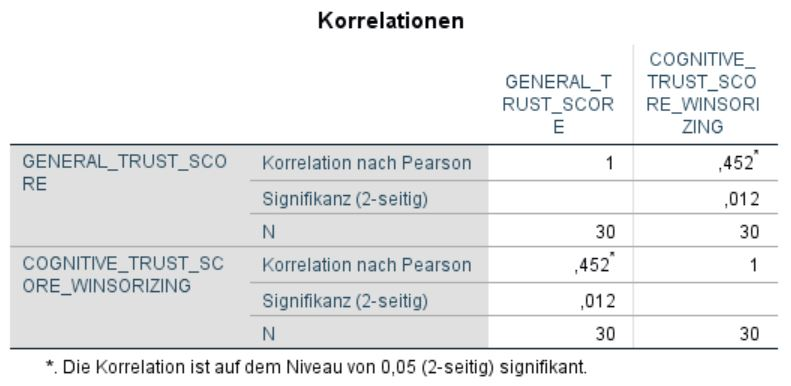
\includegraphics[scale=0.8]{Abbildungen/Post_QuestionnaireStatistiks/pearson_korrelation_general_cognitive}\\
%			\caption{Pearson-Korrelation}
%			\label{fig:pearson_korrelation}
%		\end{footnotesize}
%	\end{figure}	
	
Es ist eine signifikant positive Korrelation mittleren Effektes mit dem Pearson-Korrelationskoeffizient ($r = .452$) zwischen \ac{gt} und \ac{ct} vorhanden. 
Das generelle Vertrauen einer Person korreliert  laut Cohen \cite{cohen2013statistical} stark positiv mit dem kognitiven Vertrauen der Personen.
Weiterhin ist eine Signifikanz mit $p = .012 < \alpha = 0.05$ zu erkennen. Dies deutet darauf hin, die \textit{(Hypothese 1 / H$_{0}$)} zu verwerfen und die Alternativhypothese \textit{Hypothese 1 / H$_{1}$} anzunehmen.

\paragraph{Regressionsanalyse}
Um nun die gerichtete Annahme der positiven Auswirkung des \ac{gt} auf den \ac{ct} zu bestätigen, wurde eine Regressionsanalyse durchgeführt. Dabei wurde als unabhängige Variable \ac{gt} und als abhängige Variable \ac{ct} gewählt wurde.
%
%\begin{figure}[H]
%\centering
%		\begin{footnotesize}
%			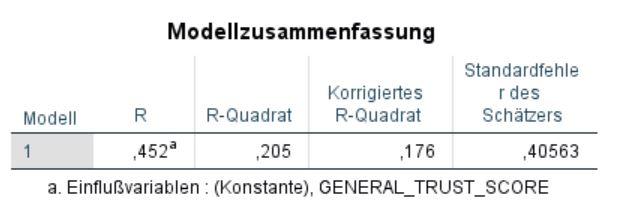
\includegraphics[scale=0.8]{Abbildungen/Post_QuestionnaireStatistiks/regression_gt_ct_modell}\\
%			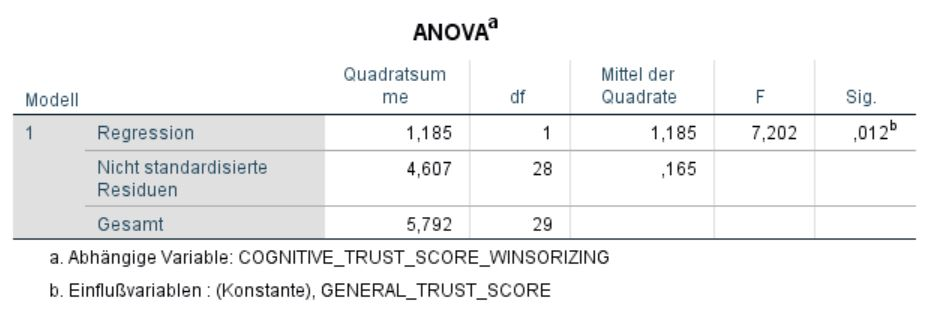
\includegraphics[scale=0.8]{Abbildungen/Post_QuestionnaireStatistiks/regression_gt_ct_anova}\\
%			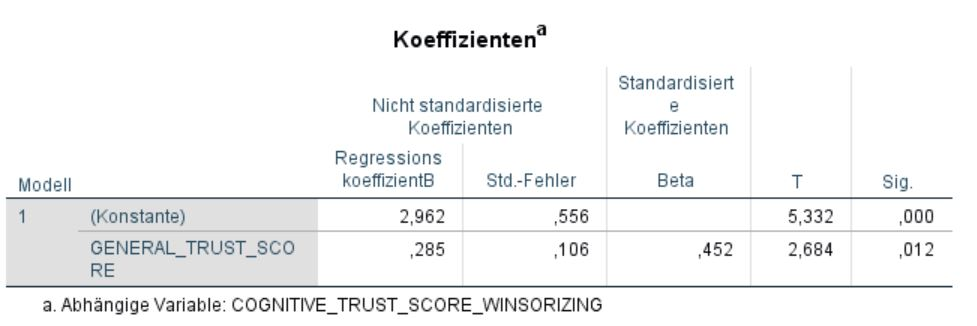
\includegraphics[scale=0.8]{Abbildungen/Post_QuestionnaireStatistiks/regression_gt_ct_koeffizienten}\\
%			\includegraphics[scale=0.5]{Abbildungen/Post_QuestionnaireStatistiks/diagramm_regression_gt_ct}\\
%			\caption{Pearson-Korrelation}
%			\label{fig:regressionsanalyse}
%		\end{footnotesize}
%	\end{figure}	

Das Bestimmtheitsmaß ($R^{2} = .205$) deutet laut \citep{cohen2013statistical} auf eine geringe bis mittlere Varianzaufklärung des \ac{ct} durch \ac{gt} hin. Somit lassen sich $20,5\%$ der Varianz unseres \ac{ct} durch den \ac{gt} erklären. \\
Der Regressionskoeffizient der Variable \ac{gt} beträgt $\beta = .452$ und ist signifikant ($t(28) = 2,684; p = .012 < \alpha = 0.05$). \\
Weiterhin ist das Ergebnis der ANOVA $F(1,28) = 7,202; p = .012 < \alpha = 0.05$ und es lässt sich \textit{Hypothese 1 / H$_{0}$} zum Signifikanzniveau $\alpha = 0.05$ verwerfen. \\
Der \ac{gt} eignet sich als Prädiktor für den \ac{ct}. Die geschätzte Zunahme an \ac{ct} beläuft sich auf $0.456$ Punkte \ac{ct} pro \ac{gt} ($\beta = 0.456; t(28) = 2,684; p = .012 < \alpha = 0.05$). \\
Der \ac{gt} erklärt zudem einen signifikanten Anteil der Varianz vom \ac{ct} ($R^{2} = .205; F(1,28) = 7,202; p = .012 < \alpha = 0.05$).


\newpage
	\subsection{Analyse Hypothese 2}
H2$_{0}$ : Die Konditionen \ac{ik} oder \ac{nik} haben \textbf{keinen Signifikant abweichenden Einfluss} auf den Cognitive-Trust-Score (\ac{ct}).\\
Es wird der Zusammenhang zwischen den unabhängigen Variablen \ac{ik} und \ac{nik} sowie \ac{cti} und \ac{ctn} auf Konditionslevel analysiert. Dazu wird ein T-Test durchgeführt. Die Gruppierungsvariablen sind dabei als \ac{ik} und \ac{nik} definiert.

%
%\begin{figure}[H]
%\centering
%		\begin{footnotesize}
%			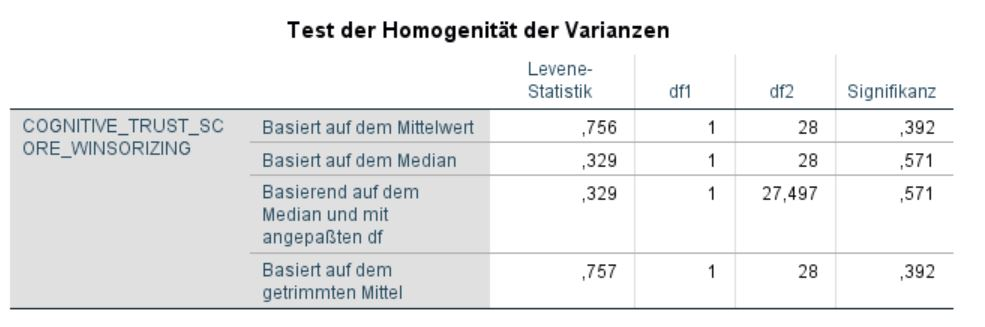
\includegraphics[scale=0.8]{Abbildungen/Post_QuestionnaireStatistiks/Varianzgleichheit_Levene_cti_ctn}
%			\caption{Levene-Test auf Varianzgleichheit von \ac{cti} und \ac{ctn}}
%			\label{fig:Varianzgleichheit_Levene_gt_ct}
%		\end{footnotesize}
%	\end{figure}	
%	
\paragraph{Normalverteilung}
\ac{ctn} ist laut Kolmogoroff-Smirnov-Test mit ($p = .2 > \alpha = 0.05$) Normalverteit. \ac{cti} ist ebenfalls laut Kolmogoroff-Smirnov-Test mit ($p = .061 > \alpha = 0.05$) Normalverteilt. 
%\ac{ct} ist laut Kolmogoroff-Smirnov-Test mit ($p = .2 > \alpha = 0.05$) Normalverteit.
Siehe \textbf{\autoref{fig:KolSmirIndNONIK}} und \textbf{\autoref{fig:KolSmirIndIK}}.

\paragraph{Varianzgleichheit}
Als nächstes wurde auf Varianzgleichheit überprüft. Der Levene-Test zeigt eine Varianzgleichheit zwischen \ac{cti} und \ac{ctn} ($L = .756; p=0.392 > \alpha = 0.05$). Damit können wir davon ausgehen, dass die Gruppen gleiche Varianzen haben. 
%	\begin{figure}[H]
%\centering
%		\begin{footnotesize}
%			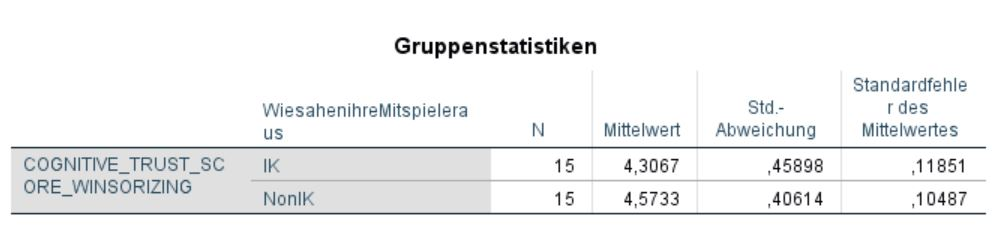
\includegraphics[width=\textwidth]{Abbildungen/Post_QuestionnaireStatistiks/h2_ttest_gruppenstatistik}
%			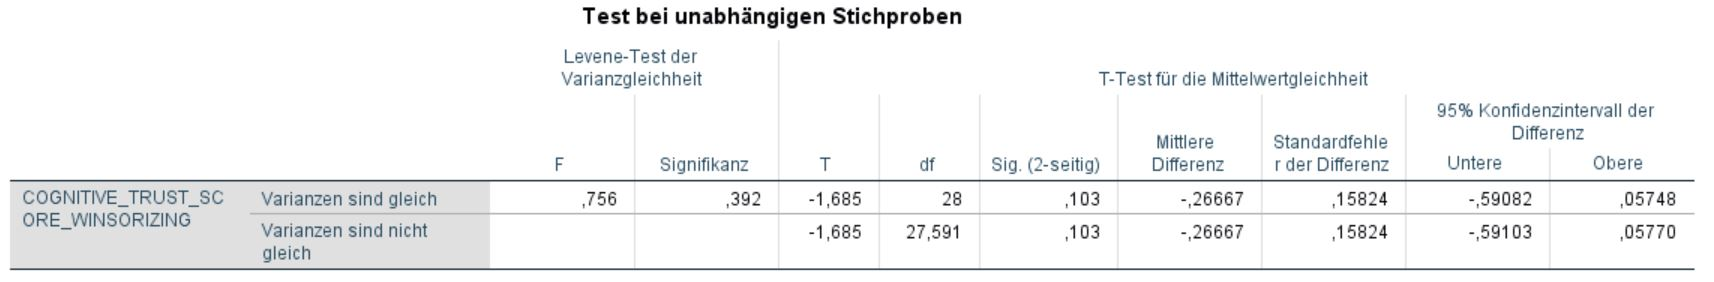
\includegraphics[width=\textwidth]{Abbildungen/Post_QuestionnaireStatistiks/ttest_cti_ctn}
%			\caption{T-Test zwischen \ac{gt} und \ac{ct} mit dem Faktor IK und NON-IK}
%			\label{fig:ttest_gt_ct}
%		\end{footnotesize}
%	\end{figure}	
\paragraph{Mittelswerte und Standardabweichungen}
Der Cognitive-Trust-Score (\ac{cti}) beträgt bei Kondition \ac{ik} im Mittel ($\tilde x = 4,306$) mit einer Standardabweichung von ($\sigma = .458$).\newline 
Der Cognitive-Trust-Score (\ac{ctn}) beträgt der Kondition \ac{nik} im Mittel ($\tilde x = 4,573$) mit einer Standardabweichung von ($\sigma = .406$).

\paragraph{t-Test}
Der T-Wert ist kleiner Null ($T = -1,685 < 0$), was auf einen Mittelwertsunterschied zwischen \ac{cti} und \ac{ctn} hinweist. Der Mittelwert $\bar(x) = 4,306$ der Kondition \ac{ik} ist kleiner als der Mittelwert $\bar(x) = 4,573$ der Kondition \ac{nik}.
Der T-Test zeigt bei der Differenz des durchschnittlichen \ac{ct} bei der Kondition \ac{ik} ($\bar(x) = 4,3067; \sigma = .45898$) und \ac{nik} ($\bar(x) = 4,5733; \sigma =.40614$) jedoch keine Signifikanz ($t(28) = -1,685; p = .103 > \alpha = 0.05$).

\paragraph{Mann-Whitney-U-Test}
Aufgrund des geringen p-Wertes des \ac{cti} im Kolmogoroff-Smirnov-Test mit ($p = .061 > \alpha = 0.05$) wurde zusätzlich noch der Mann-Whitney-U-Test durchgeführt.
Es wurde durch den Mann-Whitney-U-Test überprüft, ob sich der \ac{ct} nach Konditionen \ac{ik} oder \ac{nik} unterscheidet. Die Verteilungen der beiden Gruppen \ac{ik} und \ac{nik} unterschieden sich  laut Kolmogorov-Smirnov ($p = 0.660 > \alpha = 0.05$) nicht Signifikant von einander. Es gab keinen signifikanten Unterschied der Mediane des \ac{ct} zwischen ($\ac{ik} : \tilde x = 4.20$) und ($\ac{nik} : \tilde x = 4.60)$, ($U = 76.000, Z = -1.534, p = .127 > \alpha = 0.05, r =-0,280$). \\

Somit kann \textit{(Hypothese 2 / H$_{0}$)} nicht verworfen werden.

\newpage
\subsection{Analyse Hypothese 3}
H3$_{0}$ : Ein hoher Cognitiver-Trust-Score hat \textbf{keinen Einfluss} auf die Team-Effektivität bei unterschiedlichen Avatarverkörperungen.

\paragraph{Vertrauenstabelle pro Team}
Es wird der Zusammenhang zwischen \ac{cti} und \ac{tRoundIK} sowie \ac{ctn} und \ac{tRoundNIK} auf Team-Level analysiert.
Jeweils 3 Teammitglieder besitzen die selbe Teameffektivität, da diese die selbe Anzahl an Runden abgeschließen. Die Anzahl der abgeschlossenen Runden pro Team pro Kondition wurde zu jeweils einer Variable zusammengefasst : \ac{tRoundIK} sowie \ac{tRoundNIK}. Für jedes Team wird eine gemeinsamer Kognitiver-Vertrauenswert berechnet. Dieser sagt aus, wie viel Kognitives Vertrauen das gesamte Team untereinander besitzt. Dieser Kognitive Vertrauenswert ergibt sich aus der Summe der Kognitiven-Vertrauensangaben der einzelnen Personen eines Teams. Die Kognitiven Vertrauenswerte des Teams der unterschiedlichen Konditionen werden zu den Variablen \ac{teamCogIK} sowie \ac{teamCogNIK} zusammengefasst.
Da die individuellen Vertrauenswerte zusammengefasst wurden, wird der Ausreißer \dq{}ID 1\dq{} ignoriert und mit in die Berechnung eingezogen. Somit müssen die Kognitiven Vertrauenswerte nicht winsorisiert werden. Alle Ergebnisse werden in \ac{ik} und \ac{nik} aufgeteilt um ein Vergleich der verschiedenen Konditionen darzustellen.

\begin{table}[H]
	\centering\footnotesize\setstretch{1.2}
	\caption{Kognitive-Vertrauenswerte - Individuell und pro Team zusammengefasst}
	\label{VariableBreakdown}
	\begin{tabularx}{\textwidth}{r | p{2cm} p{1.5cm} p{1.5cm} p{1.5cm} p{1.5cm} p{1.5cm} p{1.5cm} } 
		ID & Individueller-Kognitiver Vertrauenswert & Kondition & Erfolgreich abgeschlossene Runden & Team ID & Summe \ac{ct}\\
		\hline 
		1 & $2,00$ & 1 & 4 & Team 1 & $11,00$\\
		2 & $4,60$ & 1 & 4 & &\\
		3 & $4,40$ & 1 & 4 & & \\
		\hline 
		4 & $4,00$ & 1 & 10 & Team 2 & $12,00$\\
		5 & $4,00$ & 1 & 10 & &\\
		6 & $4,00$ & 1 & 10 & &\\
		\hline 
		7 & $5,00$ & 1 & 7 & Team 3 & $13,80$\\
		8 & $3,80$ & 1 & 7 & & \\
		9 & $5,00$ & 1 & 7 & & \\
		\hline 
		10 & $5,00$ & 1 & 11 & Team 4 & $13,80$ \\
		11 & $4,00$ & 1 & 11 & & \\
		12 & $4,80$ & 1 & 11 & & \\
		\hline 
		13 & $4,20$ & 1 & 13 & Team 5 & $12,00$ \\
		14 & $4,20$ & 1 & 13 & & \\
		15 & $3,60$ & 1 & 13 & & \\
		\hline 
		16 & $5,00$ & 2 & 9 & Team 6 & $14,60$ \\
		17 & $4,60$ & 2 & 9 & &\\
		18 & $5,00$ & 2 & 9 & &\\
		\hline 
		19 & $5,00$ & 2 & 12 & Team 7 & $14,80$ \\
		20 & $4,80$ & 2 & 12 & & \\
		21 & $5,00$ & 2 & 12 & & \\
		\hline 
		22 & $4,80$ & 2 & 8 & Team 8 & $13,00$ \\
		23 & $4,40$ & 2 & 8 & & \\
		24 & $3,80$ & 2 & 8 & & \\
		\hline 
		25 & $4,20$ & 2 & 7 & Team 9 & $13,00$ \\
		26 & $4,40$ & 2 & 7 & & \\
		27 & $4,40$ & 2 & 7 & & \\
		\hline 
		28 & $4,60$ & 2 & 9 & Team 10 & $13,20$ \\
		29 & $4,80$ & 2 & 9 & &\\
		30 & $3,80$ & 2 & 9 & & \\	
	\end{tabularx}
\end{table}

\paragraph{Normalverteilung}
Laut Kolmogoroff-Smirnoff-Test sind sowohl die Summe der individuellen Kognitiven Vertrauenswerte des Teams (\ac{teamCogIK} $p = .200 > \alpha = 0.05$), (\ac{teamCogNIK} $p = .109 > \alpha = 0.05$) sowie der Anzahl der erfolgreich abgeschlossenen Runden der Teams (\ac{tRoundIK} $p = .200 > \alpha = 0.05$), (\ac{tRoundNIK} $p = .161 > \alpha = 0.05$) Normalverteilt.

\paragraph{Mittelwerte und Standardabweichungen}
Der Cognitive-Trust-Score pro Team (\ac{teamCogIK}) beträgt der Kondition \ac{ik} im Mittel ($\tilde x = 12,520$) mit einer Standardabweichung von ($\sigma = 1,237$).\newline 
Der Cognitive-Trust-Score pro Team (\ac{teamCogNIK}) beträgt der Kondition \ac{nik} im Mittel ($\tilde x = 13,72$) mit einer Standardabweichung von ($\sigma = .9011$). \newline 
Die Anzahl der Abgeschlossenen Runden pro Team (\ac{tRoundIK}) beträgt der Kondition \ac{ik} im Mittel ($\tilde x = 9$) mit einer Standardabweichung von ($\sigma = 3,535$).\newline 
 Die Anzahl der Abgeschlossenen Runden pro Team (\ac{tRoundNIK}) beträgt der Kondition \ac{nik} im Mittel ($\tilde x = 9$) mit einer Standardabweichung von ($\sigma = 1,870$). 

\paragraph{Spearman-Korrelationsanalyse}
Da eine Korrelation zwischen ($N=5$) Werten durchgeführt wird und kein linearer Zusammenhang zu erkennen ist, kommt eine Spearman-Korrelation zum Einsatz. Diese korreliert die kognitiven Vertrauenswerte des Teams und die erfolgreich abgeschlossenen Runden der Teams für beide Avatarkonditionen.

%\begin{figure}[H]
%\centering
%		\begin{footnotesize}
%			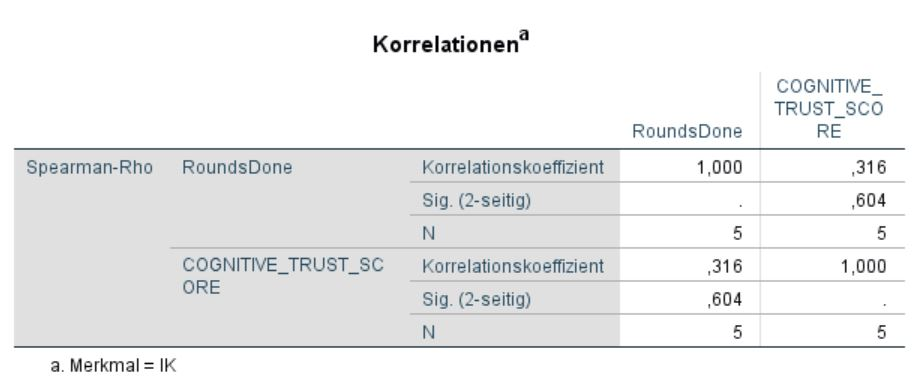
\includegraphics[scale=0.8]{Abbildungen/Post_QuestionnaireStatistiks/H3_IK_Korrelation_Spearman}
%			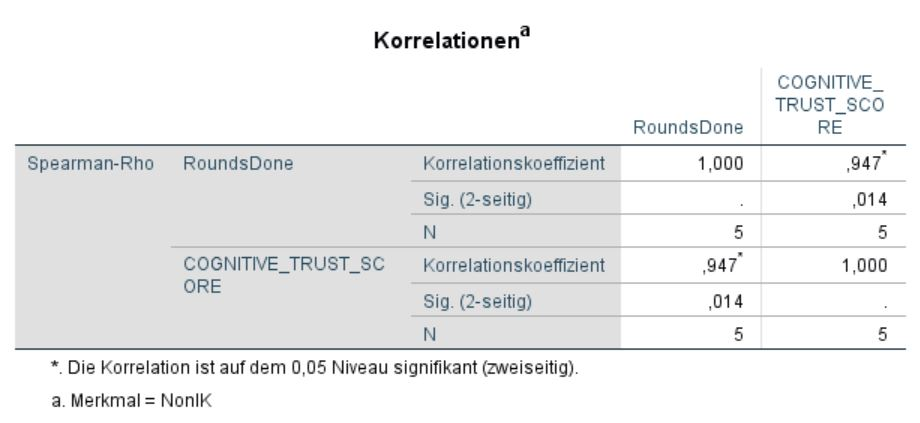
\includegraphics[scale=0.8]{Abbildungen/Post_QuestionnaireStatistiks/H3_NIK_Korrelation_Spearman}
%			\caption{Spearman-Korrelation zwischen den einzelnen Teams und dem \ac{te}}
%			\label{fig:Pearson_ik_nik_h3}
%		\end{footnotesize}
%	\end{figure}	

Es ist eine Korrelation mittlerem Effektes ($r = .316$) zwischen \ac{teamCogIK} und \ac{tRoundIK} vorhanden. Diese Korrelation ist nicht statistisch Signifikant ($p = .604 > \alpha = 0.05$)
Es ist eine positive Korrelation starken Effektes ($r = .947$) zwischen \ac{teamCogNIK} und \ac{tRoundNIK} vorhanden. Diese Korrelation ist statistisch Signifikant ($p = .014 < \alpha = 0.05$). 

\paragraph{Regressionsanalyse}
Um die nicht statistische Signifikanz zu bestätigen, wird zusätzlich eine Regressionsanalyse durchgeführt, bei der angenommen wird, dass das \ac{teamCog} einen \underline{positiven Einfluss} auf die \ac{tRound} hat.
\ac{teamCog} wird wurde als unabhängige und \ac{tRound} als abhängige Variable definiert.

\paragraph{Kondition \ac{ik}}
Das Bestimmtheitsmaß ($R^{2} = .082$) deutet laut \citep{cohen2013statistical} auf eine schwache Varianzaufklärung der \ac{tRoundIK} durch \ac{teamCogIK} hin. Somit lassen sich $8,2\%$ der Varianzen unserer \ac{tRoundIK} durch den \ac{teamCogNIK} erklären. \\
Der Regressionskoeffizient der Variable \ac{teamCogIK} beträgt ($\beta = .286$) und statistisch nicht signifikant ($t(3) = .516; p = .641 > \alpha = 0.05$). \\
Weiterhin ist das Ergebnis der ANOVA ($F(1,3) = .267; p = .641 > \alpha = 0.05$) und es lässt sich \textit{(Hypothese 3 / H$_{0}$)} zum Signifikanzniveau ($\alpha = 0.05$) für die Kondition \ac{ik} nicht verwerfen. \\
Der \ac{teamCogIK} eignet sich nicht als Prädiktor für die \ac{tRoundIK}.
Siehe \textbf{\autoref{fig:h3_regression}}

\paragraph{Kondition \ac{nik}}
Das Bestimmtheitsmaß ($R^{2} = .641$) deutet laut \citep{cohen2013statistical} auf eine sehr starke Varianzaufklärung der \ac{tRoundNIK} durch \ac{teamCogNIK} hin. Somit lassen sich $80,1\%$ der Varianzen unserer \ac{tRoundNIK} durch den \ac{teamCogNIK} erklären. \\
Der Regressionskoeffizient der Variable \ac{teamCogNIK} beträgt ($\beta = .801$) und statistisch nicht signifikant ($t(3) = 2,316; p = .103 > \alpha = 0.05$). \\
Weiterhin ist das Ergebnis der ANOVA ($F(1,3) = 5,363; p = .103 > \alpha = 0.05$) und es lässt sich \textit{(Hypothese 3 / H$_{0}$)} zum Signifikanzniveau ($\alpha = 0.05$) für die Kondition \ac{nik} nicht verwerfen. \\
Der \ac{teamCogNIK} eignet sich nicht als Prädiktor für die \ac{tRoundNIK}.
\textbf{\autoref{fig:h3_regression}}\\
Die Hypothese \textit{(Hypothese 3 / H$_{1}$)} kann somit nicht angenommen werden. Ein unterschiedlicher Kognitiver-Vertrauenswert hat keinen Einfluss auf die Team-Effektivität bei unterschiedlichen Konditionen.

\paragraph{Hypothese 3a : Analyse ohne die Aufteilung in \ac{ik} und \ac{nik} }
Da die Stichprobe mit lediglich 5 Teams pro Kondition bei der Korrelationsanalyse sowie der Regressionsanalyse zwischen \ac{teamCogIK} und \ac{tRoundIK} sowie \ac{teamCogNIK} und \ac{tRoundNIK} zu klein ist, wurde zusätzlich eine Spearman-Korrelationsanalyse sowie Regressionsanalyse \textit{ohne} die Aufteilung in die Konditionen \ac{ik} und \ac{nik} durchgeführt und somit folgende Hypothese aufgestellt :\\
H3a$_{0}$ : Ein hoher Cognitiver-Trust-Score hat \textbf{keinen Einfluss} auf die Team-Effektivität (\ac{tRound}).

Laut Kolmogoroff-Smirnoff-Test sind, ohne die Aufteilung in die Konditionen \ac{ik} und \ac{nik}, sowohl die Summe der individuellen Kognitiven Vertrauenswerte des Teams \ac{teamCog} ($p = .200 > \alpha = 0.05$) sowie der Anzahl der erfolgreich abgeschlossenen Runden der Teams \ac{tRound} ($p = .200 > \alpha = 0.05$) Normalverteilt.

Der Cognitive-Trust-Score der Teams (\ac{teamCog} beträgt im Mittel ($\tilde x = 13,12$) mit einer Standardabweichung von ($\sigma = 1,200$).
Die Anzahl der Abgeschlossenen Runden (\ac{tRound} beträgt im Mittel ($\tilde x = 9$) mit einer Standardabweichung von ($\sigma = 2,666$). 

			\paragraph{Spearman-Korrelationsanalyse}
Es ist eine positive Korrelation mittlerem Effektes mit dem Spearman-Korrelationskoeffizient ($r = .265$) zwischen \ac{teamCog} und \ac{tRound} vorhanden. Weiterhin ist keine Signifikanz ($p = .460 > \alpha = 0.05$) zu erkennen. Dies deutet darauf hin, dass die \textit{(Hypothese 3a / H3a$_{0}$)} nicht verworfen werden kann. Siehe \textbf{\autoref{fig:h3_both}}
			
			\paragraph{Regressionsanalyse}
Das Bestimmtheitsmaß ($R^{2} = .130$) deutet laut \citep{cohen2013statistical} auf eine mittlere Varianzaufklärung der \ac{tRound} durch \ac{teamCog} hin. Somit lassen sich $13,0\%$ der Varianzen unserer \ac{tRound} durch den \ac{teamCog} erklären. \\
Der Regressionskoeffizient der Variable \ac{teamCog} beträgt ($r = .361$) und ist statistisch nicht signifikant ($t(8) = 1,095; p = .306 > \alpha = 0.05$). \\
Weiterhin ist das Ergebnis der ANOVA ($F(1,8) = 1,198; p = .306 > \alpha = 0.05$) und es lässt sich \textit{(Hypothese 3 / H3a$_{0}$)} zum Signifikanzniveau ($\alpha = 0.05$) nicht verwerfen. \\
Der \ac{teamCog} eignet sich nicht als Prädiktor für die \ac{tRound}.
Siehe \textbf{\autoref{fig:h3_both}}

\newpage
	\subsection{Analyse Hypothese 4}
H4$_{0}$ : Die Konditionen \ac{ik} oder \ac{nik} haben \textbf{keinen Signifikant abweichenden Einfluss} auf die Anzahl der erfolgreich abgeschlossenen Runden \ac{tRound} eines Teams.\\
Wie in \textit{Hypothese 3} beschrieben, ist \ac{tRound} der einzelnen Teams Normalverteilt.
Um die  \textit{Hypothese 4} auszuwerten, wird ein T-Test mit 2 unabhängigen Stichproben für \ac{tRound} durchgeführt. Die Gruppierungsvariablen sind dabei \ac{ik} sowie \ac{nik}.

Die abgeschlossenen Runden pro Team (\ac{tRoundsIK}) betragen bei der Kondition \ac{ik} im Mittel ($\tilde x = 9$) mit einer Standardabweichung von ($\sigma = 3,535$).\newline 
Der abgeschlossenen Runden pro Team (\ac{tRoundsIK}) betragen bei der Kondition \ac{nik} im Mittel ($\tilde x = 9$) mit einer Standardabweichung von ($\sigma = 1,870$). \newline 
Es ist kein Mittelwertsunterschied festzustellen.

		\subsubsection{T-Test}
Der T-Wert ist gleich Null ($T = .000 = 0$), was auf keinen Mittelwertsunterschied zwischen \ac{ik} und \ac{nik} hinweist.
Die Varianzen sind mit ($L= 2.909; p = .126 > \alpha = 0.05$) gleich.
Der T-Test zeigt bei der Differenz des durchschnittlichen \ac{tRound} bei der Kondition \ac{ik} ($\bar(x) = 9; \sigma = 3,5355$) und \ac{nik} ($\bar(x) = 9; \sigma = 1,8708$) keine Signifikanz ($t(8) = .000; p = 1 > \alpha = 0.05$).\\

%\begin{figure}[H]
%\centering
%		\begin{footnotesize}
%			\includegraphics[scale=0.8]{Abbildungen/Post_QuestionnaireStatistiks/h4_ttest}
%			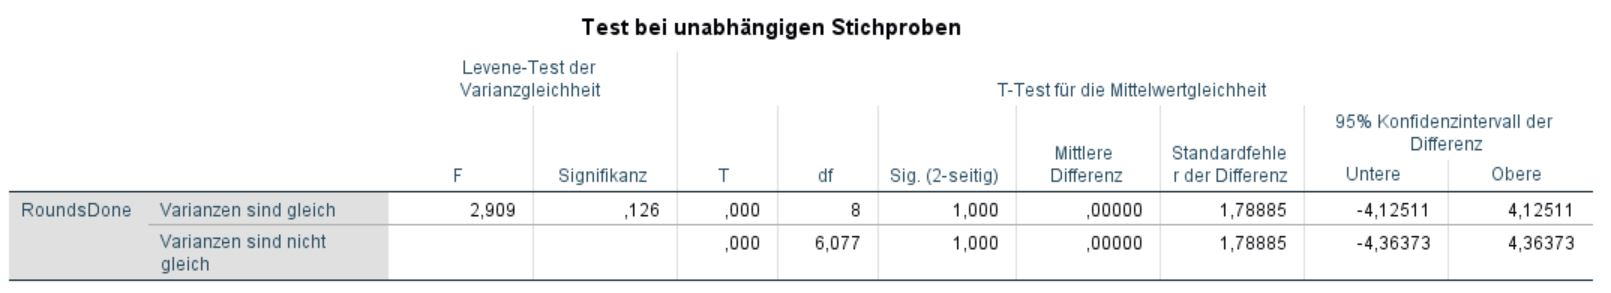
\includegraphics[scale=0.5]{Abbildungen/Post_QuestionnaireStatistiks/h4_ttest2}
%			\caption{T-Test für unabhängige Stichproben der Team-Effektivität mit den unabhängigen Variablen \ac{ik} sowie \ac{nik}}
%			\label{fig:h4_ttest}
%		\end{footnotesize}
%	\end{figure}	

Um dies zu Bestätigen und die Stichprobe zu vergrößern, wird ein weiterer T-Test durchgeführt, der nicht auf Team-Level sondern auf Konditionslevel misst. Somit erhöht sich die Stichprobe auf \ac{ik} = 15 sowie \ac{nik} = 15.

Der T-Wert ist gleich Null ($T = .000 = 0$), was auf keinen Mittelwertsunterschied zwischen \ac{ik} und \ac{nik} hinweist.
Die Varianzen sind mit ($L= 10,182; p = .003 < \alpha = 0.05$) nicht gleich.
Der T-Test (Welch-Test) zeigt bei der Differenz des durchschnittlichen \ac{tRound} bei der Kondition \ac{ik} ($\bar(x) = 9; \sigma = 3,2732$) und \ac{nik} ($\bar(x) = 9; \sigma = 1,7320$) keine Signifikanz ($t(21,270) = .000; p = 1 > \alpha = 0.05$).\\

Somit kann \textit{(Hypothese 4 / H4$_{0}$)} für \ac{ik} und \ac{nik} nicht verworfen werden.

\subsubsection{Mann-Whitney-U-Test}
Es wurde zusätzlich durch den Mann-Whitney-U-Test überprüft, ob sich \ac{tRound} nach Konditionen \ac{ik} oder \ac{nik} unterscheidet. Die Verteilungen der beiden Gruppen \ac{tRoundIK} und \ac{tRoundNIK} unterschieden sich laut Kolmogorov-Smirnov ($p = .181 > \alpha = 0.05$) nicht Signifikant von einander. Es gab keinen signifikanten Unterschied der Mediane des \ac{tRound} zwischen ($\ac{tRoundIK} : \tilde x = 10$) und ($\ac{tRoundNIK} : \tilde x = 9)$, ($U = 103,500, Z = -.377, p = .734 > \alpha = 0.05, r = -0,068$). \\


\newpage
	\subsection{Analyse Hypothese 5}
H5$_{0}$ : Teams, aufgeteilt nach Avatarverkörperungen (\ac{ik}, \ac{nik}), mit einem hohem General-Trust-Score (\ac{gt}) erzielen \textbf{keine höhere Team-Effektivität} (\ac{tRound} als die mit einem niedrigen General-Trust-Score \ac{gt}.\\
Um die Hypothese 5 auszuwerten, muss eine Tabelle wie in \textbf{Hypothese 3} aufgestellt werden, die die individuellen generellen Vertrauenswerte der Personen zu einem generellen Vertrauenswert des Teams zusammenfasst. Die durch die Tabelle erstellte Variable der Summe der individuellen generellen Vertrauenswerte wird \ac{teamGen} genannt.
Anschließend wird eine Spearman-Korrelation zwischen \ac{tRound} und \ac{teamGen} auf Teamlevel durchgeführt. Anschließend wird auf Individuallevel eine Korrelation durchgeführt um die Stichprobengröße zu erhöhen. Es folgt eine Regressionsanalyse zwischen \ac{tRound} und \ac{teamGen} um eine eventuelle vorhersage des Zusammenhangs festzustellen.

		\subsubsection{Aufstellen der generellen Vertrauenstabelle pro Team}
\begin{table}[H]
	\centering\footnotesize\setstretch{1.2}
	\caption{Kognitive-Vertrauenswerte - Individuell und pro Team zusammengefasst}
	\label{VariableBreakdown}
	\begin{tabularx}{\textwidth}{r | p{2cm} p{1.5cm} p{1.5cm} p{1.5cm} p{1.5cm} p{1.5cm} p{1.5cm}} 
		ID & Individueller genereller Vertrauenswert & Kondition & Erfolgreich abgeschlossene Runden & Team ID & Summe \ac{gt}\\
		\hline 
		1 & $4,92$ & 1 & 4 & Team 1 & $15,84$\\
		2 & $4,77$ & 1 & 4 & &\\
		3 & $6,15$ & 1 & 4 & & \\
		\hline 
		4 & $5,62$ & 1 & 10 & Team 2 & $14,62$\\
		5 & $3,46$ & 1 & 10 & &\\
		6 & $5,54$ & 1 & 10 & &\\
		\hline 
		7 & $5,92$ & 1 & 7 & Team 3 & $15,46$\\
		8 & $4,31$ & 1 & 7 & & \\
		9 & $5,23$ & 1 & 7 & & \\
		\hline 
		10 & $5,46$ & 1 & 11 & Team 4 & $14,84$ \\
		11 & $4,46$ & 1 & 11 & & \\
		12 & $4,92$ & 1 & 11 & & \\
		\hline 
		13 & $4,85$ & 1 & 13 & Team 5 & $14,23$ \\
		14 & $5,46$ & 1 & 13 & & \\
		15 & $3,92$ & 1 & 13 & & \\
		\hline 
		16 & $5,77$ & 2 & 9 & Team 6 & $17,00$ \\
		17 & $5,85$ & 2 & 9 & &\\
		18 & $5,38$ & 2 & 9 & &\\
		\hline 
		19 & $4,46$ & 2 & 12 & Team 7 & $15,46$ \\
		20 & $4,77$ & 2 & 12 & & \\
		21 & $6,23$ & 2 & 12 & & \\
		\hline 
		22 & $5,46$ & 2 & 8 & Team 8 & $15,23$ \\
		23 & $4,62$ & 2 & 8 & & \\
		24 & $5,15$ & 2 & 8 & & \\
		\hline 
		25 & $4,69$ & 2 & 7 & Team 9 & $16,92$ \\
		26 & $6,08$ & 2 & 7 & & \\
		27 & $6,15$ & 2 & 7 & & \\
		\hline 
		28 & $6,00$ & 2 & 9 & Team 10 & $15,76$ \\
		29 & $5,38$ & 2 & 9 & &\\
		30 & $4,38$ & 2 & 9 & & \\	
	\end{tabularx}
\end{table}

Laut Kolmogoroff-Smirnoff-Test sind sowohl die Summe der individuellen generellen Vertrauenswerte des Teams (\ac{teamGen} $p = .200 > \alpha = 0.05$), sowie die Anzahl der erfolgreich abgeschlossenen Runden der Teams (\ac{tRound} $p = .200 > \alpha = 0.05$) Normalverteilt.
Zu dem selben Ergebnis kommt auch der Shapiro-Wilk-Test mit (\ac{teamGen} $p = .548 > \alpha = 0.05$) und (\ac{tRound} $p = .953 > \alpha = 0.05$).

Für \ac{tRound} ist $ z_{Skewness} = -0,448 $ und $z_{Kurtosis} = 0.0217$. Somit ist tRound Normalverteilt.
Für \ac{teamGen} ist $ z_{Skewness} = 0,676 $ und $z_{Kurtosis} = -0.2653$. Somit ist teamGen Normalverteilt.

Der General-Trust-Score pro Team (\ac{teamGenIK}) beträgt der Kondition \ac{ik} im Mittel ($\tilde x = 14,998$) mit einer Standardabweichung von ($\sigma = 0,648$).\newline 
Der General-Trust-Score pro Team (\ac{teamGenNIK}) beträgt der Kondition \ac{nik} im Mittel ($\tilde x = 16,074$) mit einer Standardabweichung von ($\sigma = .830$). \newline 
Die Anzahl der Abgeschlossenen Runden pro Team (\ac{tRoundIK}) beträgt der Kondition \ac{ik} im Mittel ($\tilde x = 9$) mit einer Standardabweichung von ($\sigma = 3,535$).\newline 
 Die Anzahl der Abgeschlossenen Runden pro Team (\ac{tRoundNIK}) beträgt der Kondition \ac{nik} im Mittel ($\tilde x = 9$) mit einer Standardabweichung von ($\sigma = 1,870$). 



		\subsubsection{Spearman-Korrelationsanalyse}
Aufgrund der geringen Stichprobengröße von ($N=5$) wird eine Spearman-Korrelation zwischen den generellen Vertrauenswerten des Teams \ac{teamGen} und den erfolgreich abgeschlossenen Runden durchgeführt und in die unabhängigen Variablen \ac{ik} und \ac{nik} aufgeteilt.
%
%\begin{figure}[H]
%\centering
%		\begin{footnotesize}
%			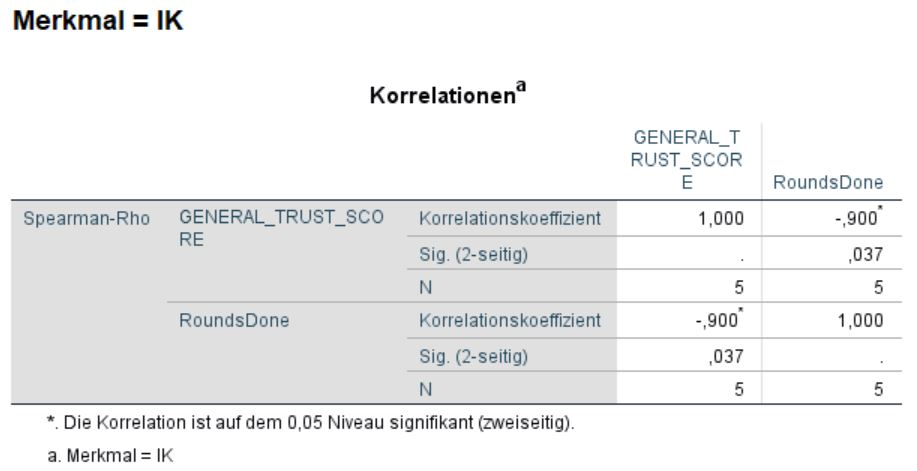
\includegraphics[scale=0.8]{Abbildungen/Post_QuestionnaireStatistiks/h5_korr_spearman_ik}
%			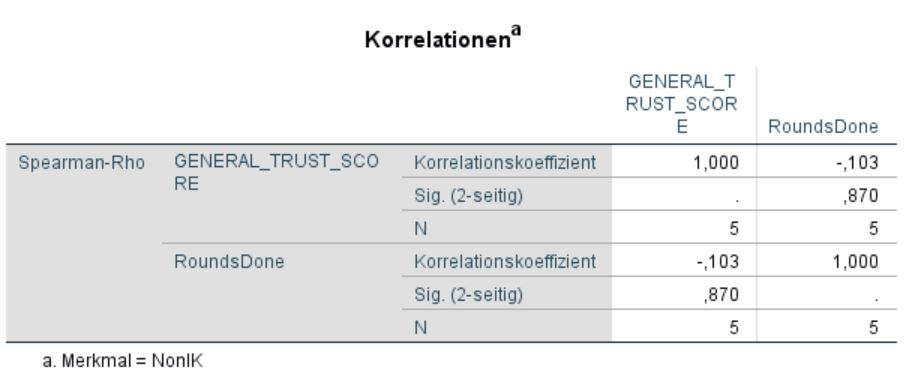
\includegraphics[scale=0.8]{Abbildungen/Post_QuestionnaireStatistiks/h5_korr_spearman_nik}
%			\caption{Pearson-Korrelation zwischen den einzelnen Teams und dem \ac{te}}
%			\label{fig:Pearson_ik_nik_h3}
%		\end{footnotesize}
%	\end{figure}	

Es ist eine negative Korrelation sehr starkem Effekt ($r = -.900$) zwischen \ac{teamGenIK} und \ac{tRoundIK} vorhanden. Diese Korrelation ist statistisch Signifikant ($p = .037 < \alpha = 0.05$)
Weiterhin ist eine negative Korrelation schwachen Effekt ($r = -.103$) zwischen \ac{teamGenNIK} und \ac{tRoundNIK} vorhanden. Diese Korrelation ist statistisch nicht Signifikant ($p = .870 > \alpha = 0.05$).

		\subsubsection{Regressionsanalyse}
Um die statistische Signifikanz des Zusammenhangs zwischen \ac{tRoundIK} und \ac{teamGenIK} und die nicht statistische Signifikanz des Zusammenhangs der Kondition \ac{nik} zwischen \ac{tRoundNIK} und \ac{teamGenNIK} zu bestätigen, wird zusätzlich eine Regressionsanalyse durchgeführt.
\ac{teamGen} wird wurde als unabhängige und \ac{tRound} als abhängige Variable definiert.

\paragraph{Kondition \ac{ik}}
Das Bestimmtheitsmaß ($R^{2} = .971$) deutet laut \citep{cohen2013statistical} auf eine sehr starke Varianzaufklärung der \ac{tRoundIK} durch \ac{teamGenIK} hin. Somit lassen sich $97,1\%$ der Varianzen unserer \ac{tRoundIK} durch den \ac{teamGenIK} erklären. \\
Der Regressionskoeffizient der Variable \ac{teamGenIK} beträgt ($r = -.971$) und ist statistisch signifikant ($t(3) = -7,040; p = .006 < \alpha = 0.01$). \\
Weiterhin ist das Ergebnis der ANOVA ($F(1,3) = 49,568; p = .006 < \alpha = 0.01$) und es lässt sich \textit{(Hypothese 5 / H$_{0}$)} zum Signifikanzniveau ($\alpha = 0.01$) für die Kondition \ac{ik} verwerfen. \\
Der \ac{teamGenIK} eignet sich als Prädiktor für \ac{tRoundIK}. Die geschätzte Abnahme an \ac{tRoundIK} beläuft sich auf $-.971$ Punkte \ac{tRoundIK} pro \ac{teamGenIK} ($\beta = -.971; t(3) = -7,040; p = .006 < \alpha = 0.01$). \\
Siehe \textbf{\autoref{fig:h5_regression}}

\paragraph{Kondition \ac{nik}}
Das Bestimmtheitsmaß ($R^{2} = .187$) deutet laut \citep{cohen2013statistical} auf eine schwache Varianzaufklärung der \ac{tRoundNIK} durch \ac{teamGenNIK} hin. Somit lassen sich $18,7\%$ der Varianzen unserer \ac{tRoundNIK} durch den \ac{teamGenNIK} erklären. \\
Der Regressionskoeffizient der Variable \ac{teamGenNIK} beträgt ($r = -.433$) und ist statistisch nicht Signifikant ($t(3) = -.831; p = .467 > \alpha = 0.05$). \\
Weiterhin ist das Ergebnis der ANOVA ($F(1,3) = .691; p = .467 > \alpha = 0.05$) und es lässt sich \textit{(Hypothese 5 / H$_{0}$)} zum Signifikanzniveau ($\alpha = 0.05$) für die Kondition \ac{nik} nicht verwerfen. \\
\ac{teamGenNIK} eignet sich nicht als Prädiktor für die \ac{tRoundNIK}.\\
\textbf{\autoref{fig:h5_regression}}

Die Hypothese \textit{(Hypothese 5 / H$_{0}$)} kann somit nicht angenommen werden, da ein abnehmender Effekt auf die \ac{tRound} pro Team durch die Konditionen \ac{ik} und \ac{nik} festgestellt wurde.

\subsubsection{Hypothese 5a :Analyse ohne die Aufteilung in \ac{ik} und \ac{nik}}
H5a$_{0}$ : Teams mit einem hohem General-Trust-Score (\ac{gt}) erzielen \textbf{keine höhere Team-Effektivität} (\ac{tRound} als die mit einem niedrigen General-Trust-Score \ac{gt}.\\
Da die Stichprobengröße mit lediglich 5 Teams pro Kondition bei der Korrelationsanalyse sowie der Regressionsanalyse zu wenig sind, wurde zusätzlich noch eine Korrelationsanalyse sowie Regressionsanalyse \textit{ohne} die Aufteilung in die Konditionen \ac{ik} und \ac{nik} durchgeführt.

Laut Kolmogoroff-Smirnoff-Test sind, ohne die Aufteilung in die Konditionen \ac{ik} und \ac{nik}, sowohl die Summe der individuellen generellen Vertrauenswerte des Teams \ac{teamGen} ($p = .200 > \alpha = 0.05$) sowie der Anzahl der erfolgreich abgeschlossenen Runden der Teams \ac{tRound} ($p = .200 > \alpha = 0.05$) Normalverteilt.

Der generelle Trust-Score der Teams (\ac{teamGen} beträgt im Mittel ($\tilde x = 15,536$) mit einer Standardabweichung von ($\sigma = .902$).
Die Anzahl der Abgeschlossenen Runden (\ac{tRound} beträgt im Mittel ($\tilde x = 9$) mit einer Standardabweichung von ($\sigma = 2,666$). 

			\paragraph{Spearman-Korrelationsanalyse}
Es ist eine unsignifikante negative Korrelation mittlerem Effektes mit dem Pearson-Korrelationskoeffizient ($r = -.627$) zwischen \ac{teamGen} und \ac{tRound} vorhanden. Weiterhin ist keine Signifikanz ($p = .052 > \alpha = 0.05$) zu erkennen. Dies deutet darauf hin, dass die \textit{(Hypothese 5 / H$_{0}$)} nicht verworfen werden kann. Siehe \textbf{\autoref{fig:h5_both}}
			
			\paragraph{Regressionsanalyse}
Das Bestimmtheitsmaß ($R^{2} = .286$) deutet laut \citep{cohen2013statistical} auf eine hohe Varianzaufklärung der \ac{tRound} durch \ac{teamGen} hin. Somit lassen sich $28,6\%$ der Varianzen unserer \ac{tRound} durch den \ac{teamGen} erklären. \\
Der Regressionskoeffizient der Variable \ac{teamGen} beträgt ($r = -.535$) und ist statistisch nicht signifikant ($t(8) = -1,791; p = .111 > \alpha = 0.05$). \\
Weiterhin ist das Ergebnis der ANOVA ($F(1,8) = 3,206; p = .111 > \alpha = 0.05$) und es lässt sich \textit{(Hypothese 5 / H$_{0}$)} zum Signifikanzniveau ($\alpha = 0.05$) nicht verwerfen. \\
Der \ac{teamGen} eignet sich nicht als Prädiktor für die \ac{tRound}.\\
Siehe \textbf{\autoref{fig:h5_both}}

\newpage
\subsection{Analyse weiterer Variablen}
Zusätzlich wurden alle weiteren, durch den Fragebogen erhobenen Variablen auf Signifikante Mittelwertsunterschiede und Mediansunterschiede sowie auf Signifikante Korrelationen überprüft.

\paragraph{Signifikante unterschiede des Medians}
Es sind Signifikante Mittelwertsunterschiede bei der Variable \ac{tc} durch den t-Test sowie dem Mann-Whitney-U-Test zu erkennen.
Es wurde durch den Mann-Whitney-U-Test überprüft, ob sich \ac{tc} nach Konditionen \ac{ik} oder \ac{nik} unterscheidet. Die Verteilungen der beiden Gruppen \ac{tci} und \ac{tcn} unterschieden sich laut Kolmogorov-Smirnov ($p = .925 > \alpha = 0.05$) nicht Signifikant von einander. Es gab einen signifikanten Unterschied der Mediane des \ac{tc} zwischen ($\ac{tci} : \tilde x = 12,23$) und ($\ac{tcn} : \tilde x = 18,77)$, ($U = 63,500, Z = -2,062, p = .039 < \alpha = 0.05$).

\paragraph{Signifikante Korrelationen}
Es wurden signifikante Zusammenhänge mittels Spearman-Rho-Korrelation auf \underline{Individualebene} zwischen folgenden Variablen gefunden :\newline
\acs{te} und \acs{tc} mit ($r = .695, p = .000 < \alpha = 0.05$)\newline
\acs{te} und \acs{ct} mit ($r = .588, p = .001 < \alpha = 0.05$)\newline
\acs{te} und \acs{cp} mit ($r = -.369, p = .045 < \alpha = 0.05$)\newline
\acs{tc} und \acs{ct} mit ($r = .436, p = .016 < \alpha = 0.05$)\newline
\acs{scp} und \acs{ipq} mit ($r = .585, p = .001 < \alpha = 0.05$)\newline
\acs{tp} und \acs{ipq} mit ($r = .723, p = .000 < \alpha = 0.05$)\newline
\acs{sp} und \acs{cp} mit ($r = .869, p = .000 < \alpha = 0.05$)\newline

Es wurden signifikante Zusammenhänge mittels Spearman-Rho-Korrelation auf \underline{Konditionsebene} zwischen folgenden Variablen gefunden :\\
\underline{\ac{ik}} :\newline
\acs{tei} und \ac{tci} mit ($r = .767, p = .001 < \alpha = 0.05$)\newline
\acs{scpi} und \acs{ipqi} mit ($r = .515, p = .050 < \alpha = 0.05$)\newline
\acs{tpi} und \acs{ipqi} mit ($r = .747, p = .001 < \alpha = 0.05$)\newline
\acs{spi} und \acs{cpi} mit ($r = .884, p = .000 < \alpha = 0.05$)\newline
\acs{tlxi} und \acs{cpi} mit ($r = .574, p = .048 < \alpha = 0.05$)\newline
\acs{tlxi} und \acs{tci} mit ($r = .652, p = .008 < \alpha = 0.05$)\newline
\acs{tlxi} und \acs{tei} mit ($r = .555, p = .032 < \alpha = 0.05$)\newline
\newline
\underline{\ac{nik}} :\newline
\acs{ten} und \acs{tcn} mit ($r = .635, p = .011 < \alpha = 0.05$)\newline
\acs{ten} und \acs{ctn} mit ($r = .767, p = .001 < \alpha = 0.05$)\newline
\acs{ten} und \acs{cpn} mit ($r = -.647, p = .009 < \alpha = 0.05$)\newline
\acs{tcn} und \acs{ctn} mit ($r = .630, p = .012 < \alpha = 0.05$)\newline
\acs{scpn} und \acs{ipqn} mit ($r = .681, p = .005 < \alpha = 0.05$)\newline
\acs{tpn} und \acs{ipqn} mit ($r = .583, p = .022 < \alpha = 0.05$)\newline
\acs{spn} und \acs{cpn} mit ($r = .884, p = .000 < \alpha = 0.05$)\newline
%
%\subsection{Analyse Hypothese 7}
%

%Unterschiedliche wahrgenommene Teameffektivität bei unterschiedlichen Avatarkonditionen.

%Auch interessant : T-Test zwischen COPRÄSENZ und WieSahenIhreMitspielerAus
%
%Auch interessant : Wie wirkt sich gt und CT gemeinsam auf TE aus? ( Auch im Team )
%
%Auch interssant : Rounds Done im Verhältnis zu Team-Effectiveness-Scale
%Auch interessant : Wie ist das Verhältnis von gedachtem Effektivitätswert zu eigentlichem tRounds?
%
%
%Auch interessant : NASA-TLX( WIE ANSTRENGEND WAR ES?) zur Round-Efficiency
%
%Auch interessant : T-Test von Team-Communication bei den IK und NON IK Gruppen
%	Hier Signifikanten unterschied der Mittelwerte gefunden!
%	
%Auch interessant : Team-Communication zur Rounds Done

-------------------------------------------------------------------------------
% WAR MEHR PRÄSENZ BEI IK ODER NIK AVATAR VORHANDEN?
%KAPITEL : VR - Präsenz in Virtual Reality

%KAPITEL : Vertrauen als Zustand - Kognitives und Affektives Vertrauen
%Ich glaube, ich habe die Aufgaben des Versuchsleiters gut erledigt -> Auf Kognitives Vertrauen analisieren Pro person! Hier ist einseitige Signifikanz in der Korrelation von Wie Erfolgreich haben Sie ihrer Meinung nach die vom Versuchleiter ... mit Cog_Trust_Windsorizing vorhanden!

% Self-Avatare

%Jedoch wurde ein größeres Gefühl von Zusammenheit festgestellt, wenn mit einem Menschenähnlichem Avatar interagiert wurde. \citep{kerr1983motivation}
%Dies auch evenntl überprüfen?
\subsection{Berechnung der Werte für die Auswertung}
Bspw. Wie wurde CT oder GT etc. berechnet? UND WARUM BENÖTIGE ICH DIESE? WARUM Z.B. BESTANDENE TEAMRUNDEN ? -> WEIL NUR SO TEAMBUILDING ERFOLG GEMESSEN WERDEN KANN
\newpage

\clearpage
\newpage

\section{Diskussion}
	\subsection{Diskussion der Ergebnisse}
	Diese Studie trägt dazu bei, besser zu verstehen, durch welche Avatarkonditionen virtuelle Teams in einem \ac{sve} effektiver Arbeiten. Durch die Berücksichtigung vom aktuellen Stand der Vertrauensforschung, wurde das aufgebaute Vertrauen der einzelnen Personen und des gesamtem Teams gemessen. Insgesamt wurde jedoch nur 1 der 5 aufgestellten Hypothesen unterstützt. 
%Anhand dieser, durch ein Experiment mit $N=30$ teilnehmenden Personen, gewonnenen Ergebnisse, wurde versucht zu verstehen, ob Teams durch einen \ac{ik} oder \ac{nik} Avatar effektiver Arbeiten. 
Anstatt eine neue Theorie zu entwickeln, wurde auf bisherigen Forschungen und Erkenntnissen aufgebaut und diese Versucht in der \ac{vr} zu evaluieren.
Die Studie stellt fest, dass das Kognitive Vertrauen (H3) sowie das generelle Vertrauen (H5) die Teameffektivität, auf Teamebene sowie auf Individualebene (H3a, H5a), nicht signifikant beeinflussen. 
Weiterhin geht hervor, dass unterschiedliche Avatarkonditionen das Kognitive-Vertrauen (H2) oder die Teameffektivität(H4) nicht signifikant beeinflussen. Diese beiden Hypothesen sind die wichtigsten Erkenntnisse dieser Studie.
Jedoch konnte durch (H1) gezeigt werden, dass, je höher der generelle Hang zum Vertrauen einer Person ist, desto eher wird an die Zuverlässigkeit und Leistungsfähigkeit des Teams geglaubt.


	Was habe ich gemacht?
	Was habe ich gefunden? 
	Was bedeutet das genau?
	\subsection{Diskussion der eingesetzten Methoden}
	\subsection{Auswirkungen auf die Gegenwart}
	\subsection{Vorschläge für zukünftige Untersuchungen}
		Social Identity und Teambuilding - Ein Avatar ist anders.
	
\section{Fazit}
\newpage

\bibliographystyle{dcu}
\bibliography{bibfile}

	\newpage
	\appendix	
\section*{Anhang}\markboth{Anhang}{Anhang}\addcontentsline{toc}{section}{Anhang}

\section{Auswertungsergebnisse}
	
	\begin{figure}[H]
	\centering
		\begin{footnotesize}
			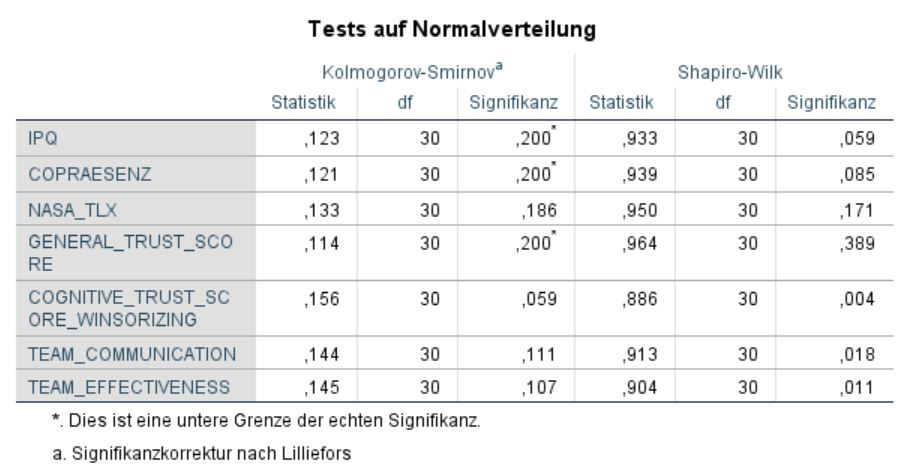
\includegraphics[scale=0.6]{Abbildungen/Post_QuestionnaireStatistiks/Normalverteilung_30}\\
			\caption{Kolmogorov-Smirnoff Normalverteilung für Individuelle Stichproben}
			\label{fig:KolSmirInd}
		\end{footnotesize}
	\end{figure}	
	
	\begin{figure}[H]
	\centering
		\begin{footnotesize}
			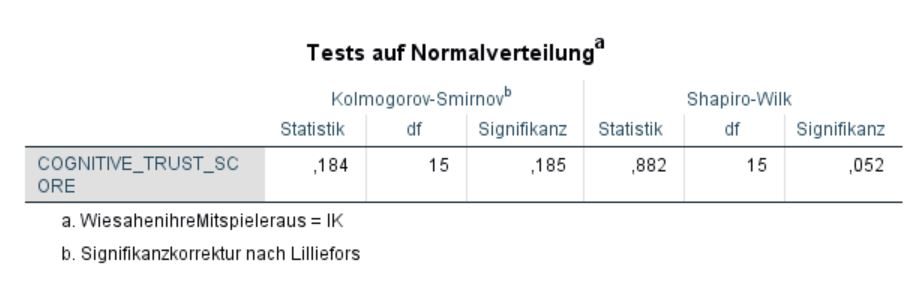
\includegraphics[scale=0.6]{Abbildungen/Post_QuestionnaireStatistiks/Normalverteilung_15_IK}\\
			\caption{Kolmogorov-Smirnoff Normalverteilung für die IK-Kondition}
			\label{fig:KolSmirIndIK}
		\end{footnotesize}
	\end{figure}	
	
	\begin{figure}[H]
	\centering
		\begin{footnotesize}
			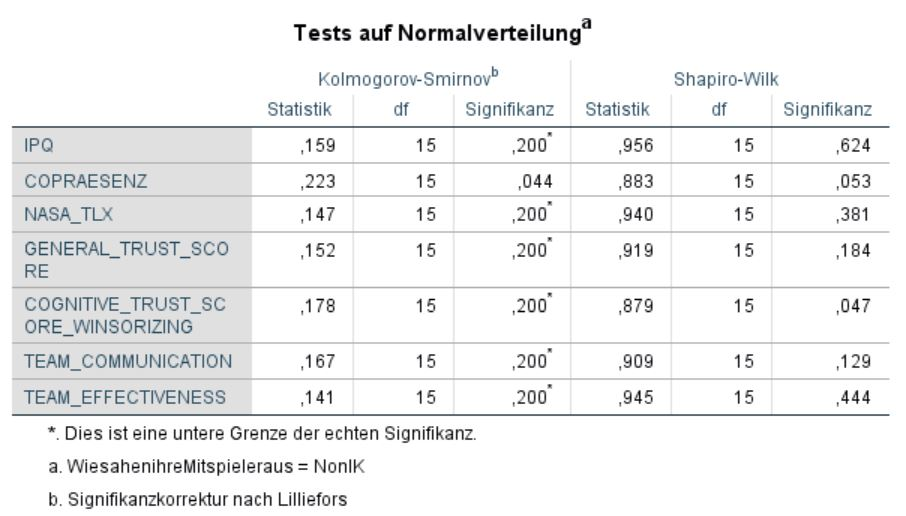
\includegraphics[scale=0.6]{Abbildungen/Post_QuestionnaireStatistiks/Normalverteilung_15_NON_IK}\\
			\caption{Kolmogorov-Smirnoff Normalverteilung für die NON-IK-Kondition}
			\label{fig:KolSmirIndNONIK}
		\end{footnotesize}
	\end{figure}	
	
	
\begin{figure}[H]
\centering
		\begin{footnotesize}
			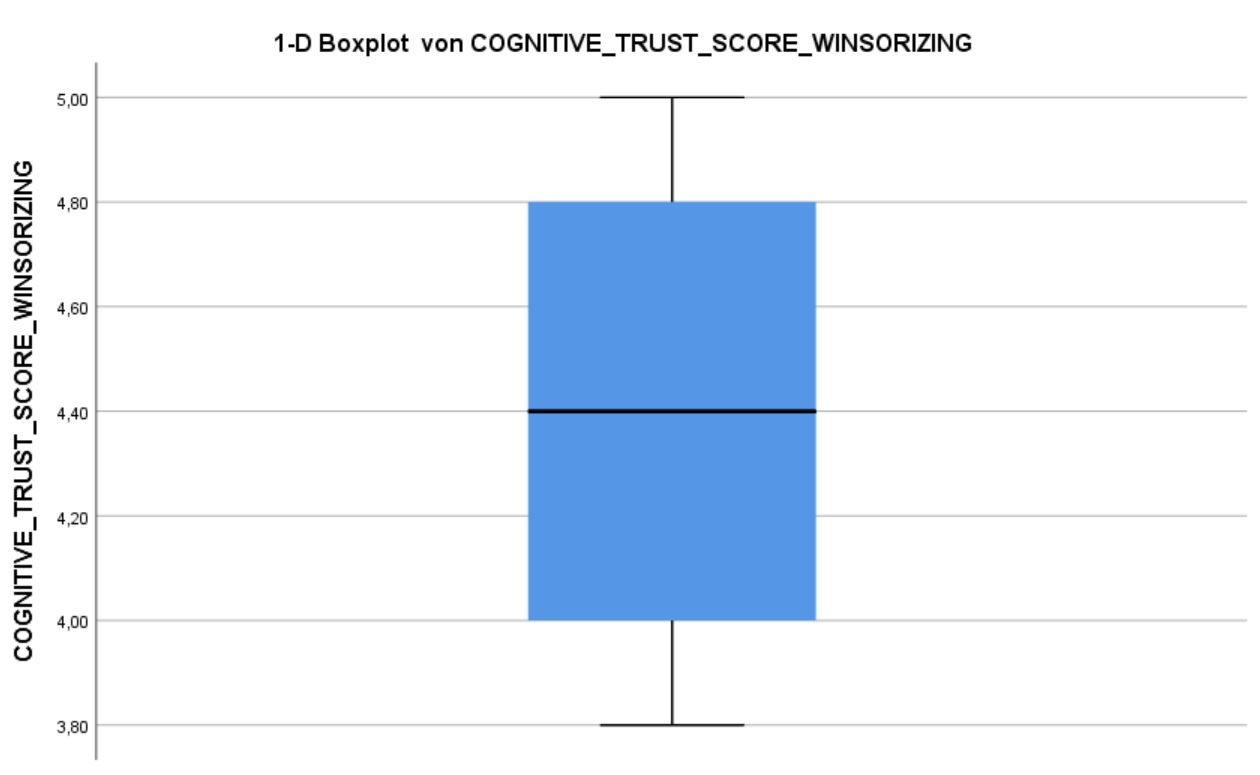
\includegraphics[scale=0.5]{Abbildungen/Post_QuestionnaireStatistiks/boxplot_cognitive_trust_winsorisiert}\\
			\caption{Boxplot kognitives Vertrauen winsorisiert}
			\label{fig:boxplot_cognitive_trust_winsorisiert}
		\end{footnotesize}
	\end{figure}	

\begin{figure}[H]
\centering
		\begin{footnotesize}
			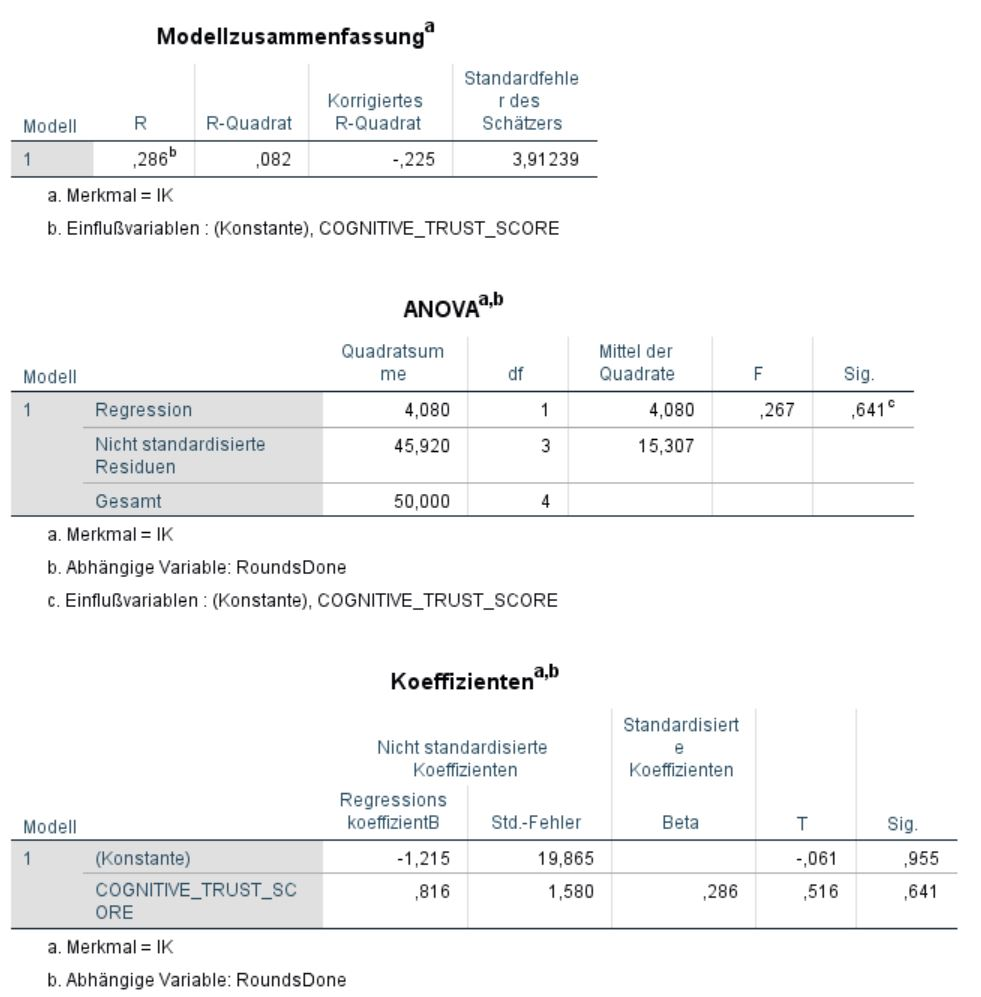
\includegraphics[scale=0.6]{Abbildungen/Post_QuestionnaireStatistiks/h3_regression_ik}
			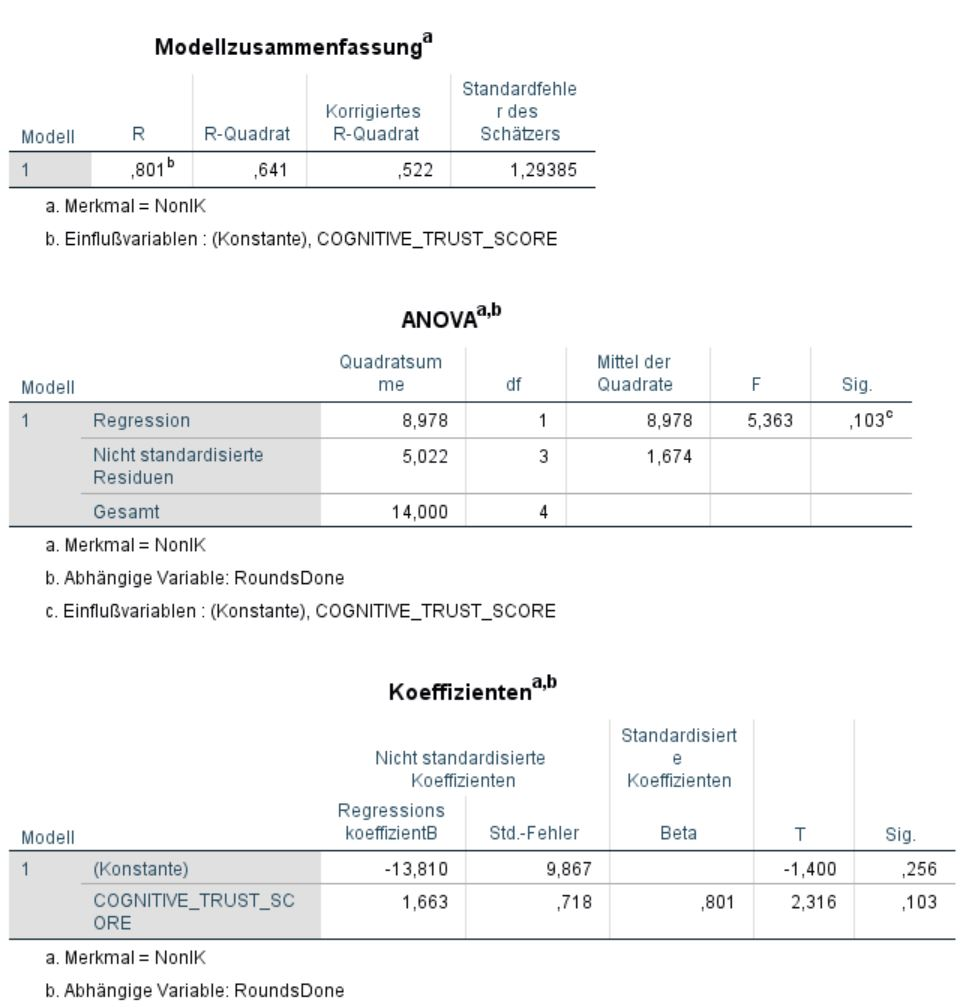
\includegraphics[scale=0.6]{Abbildungen/Post_QuestionnaireStatistiks/h3_regression_nik}
			\caption{Regressionsergebnisse der Regressionen \ac{cti} und \ac{tei} sowie \ac{ctn} und \ac{ten} }
			\label{fig:h3_regression}
		\end{footnotesize}
	\end{figure}	
	
\begin{figure}[H]
\centering
		\begin{footnotesize}
%			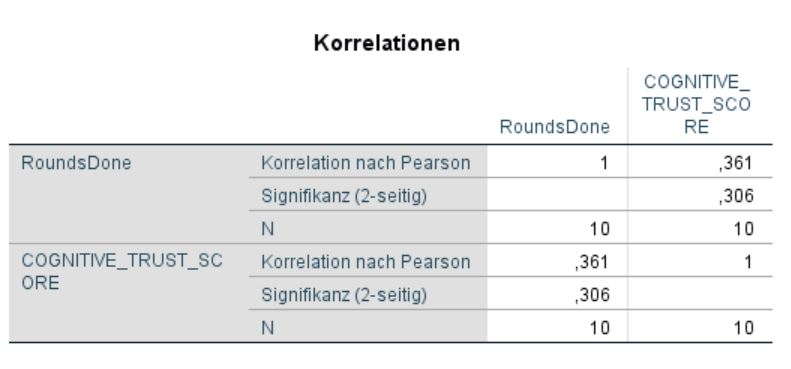
\includegraphics[scale=0.6]{Abbildungen/Post_QuestionnaireStatistiks/h3_both_korrelation}
			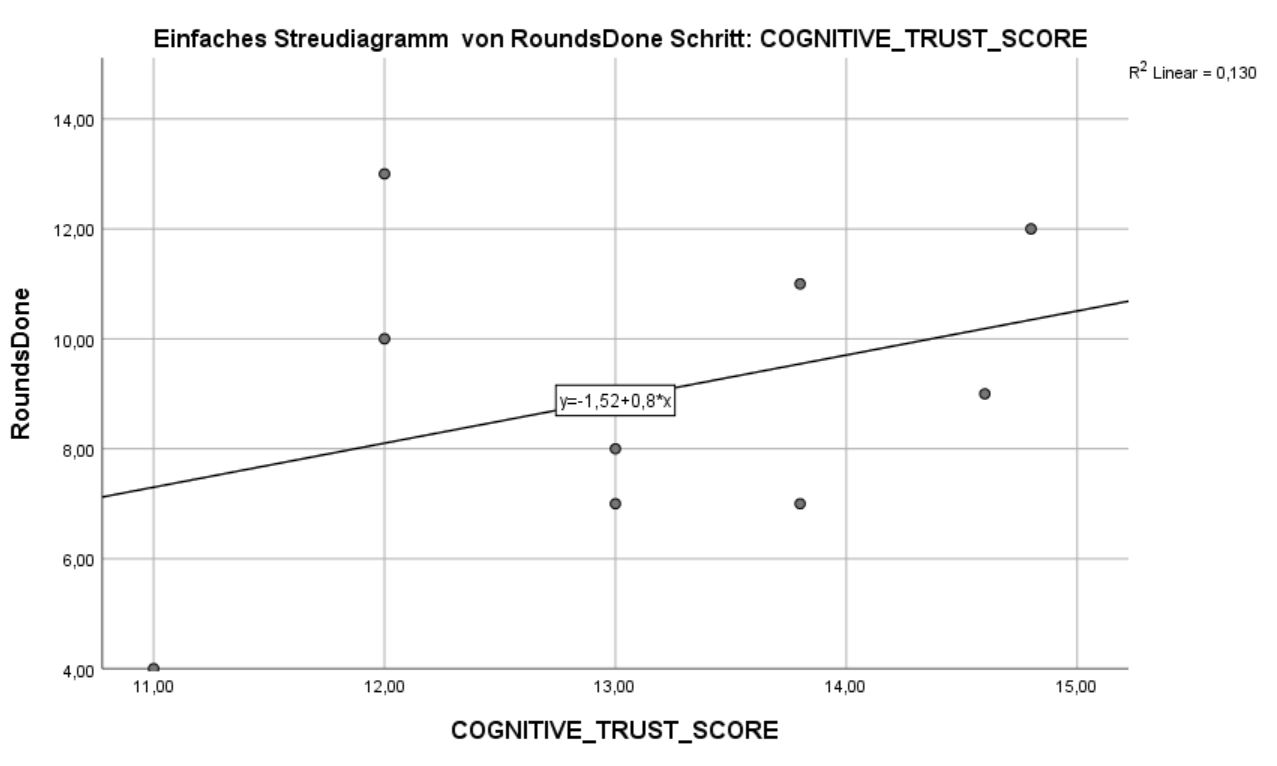
\includegraphics[scale=0.6]{Abbildungen/Post_QuestionnaireStatistiks/h3_both_diagramm_korr}
			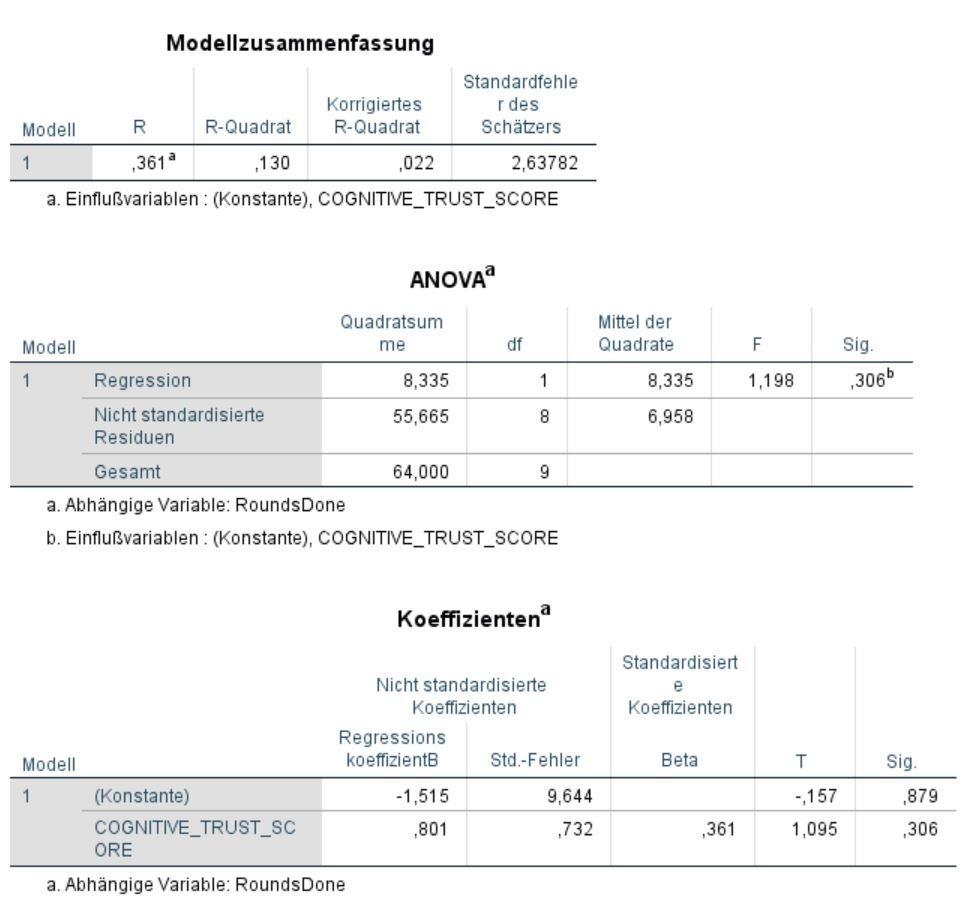
\includegraphics[scale=0.6]{Abbildungen/Post_QuestionnaireStatistiks/h3_both_regression}
			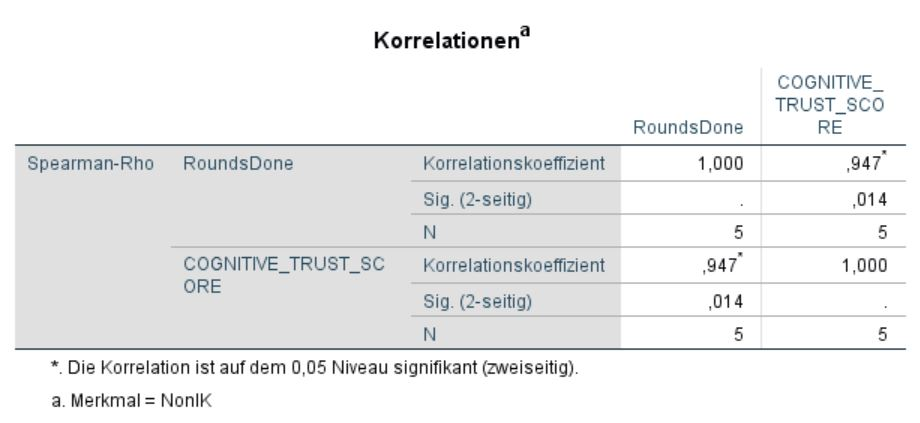
\includegraphics[scale=0.6]{Abbildungen/Post_QuestionnaireStatistiks/H3_NIK_Korrelation_Spearman}
			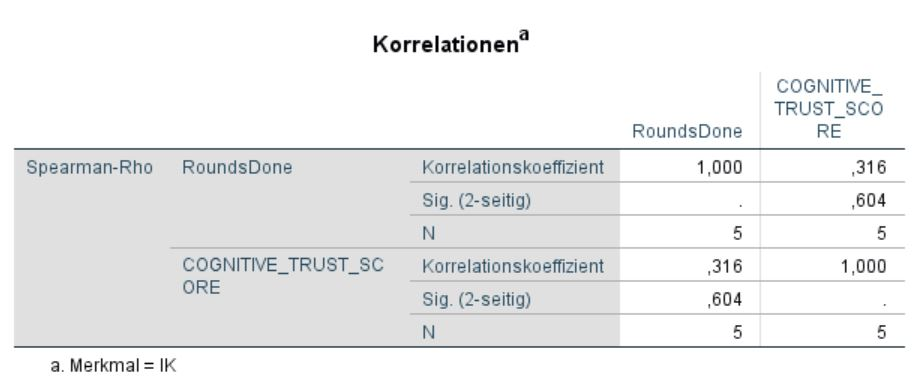
\includegraphics[scale=0.6]{Abbildungen/Post_QuestionnaireStatistiks/H3_IK_Korrelation_Spearman}
			\caption{Regressionsergebnisse der Regressionen \ac{ct} und \ac{te} }
			\label{fig:h3_both}
		\end{footnotesize}
	\end{figure}	
	
	
\begin{figure}[H]
\centering
		\begin{footnotesize}
			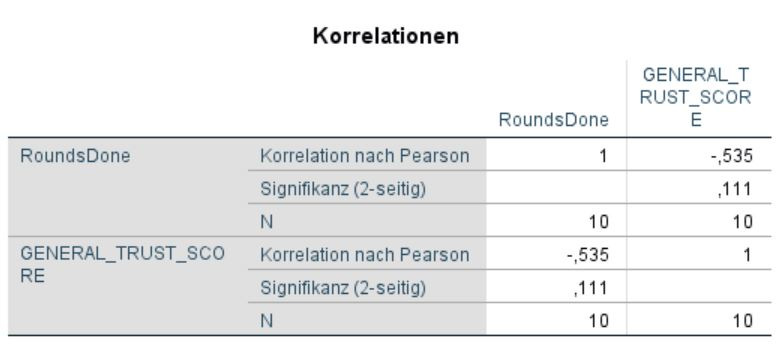
\includegraphics[scale=0.6]{Abbildungen/Post_QuestionnaireStatistiks/h5_both_korrelation}
			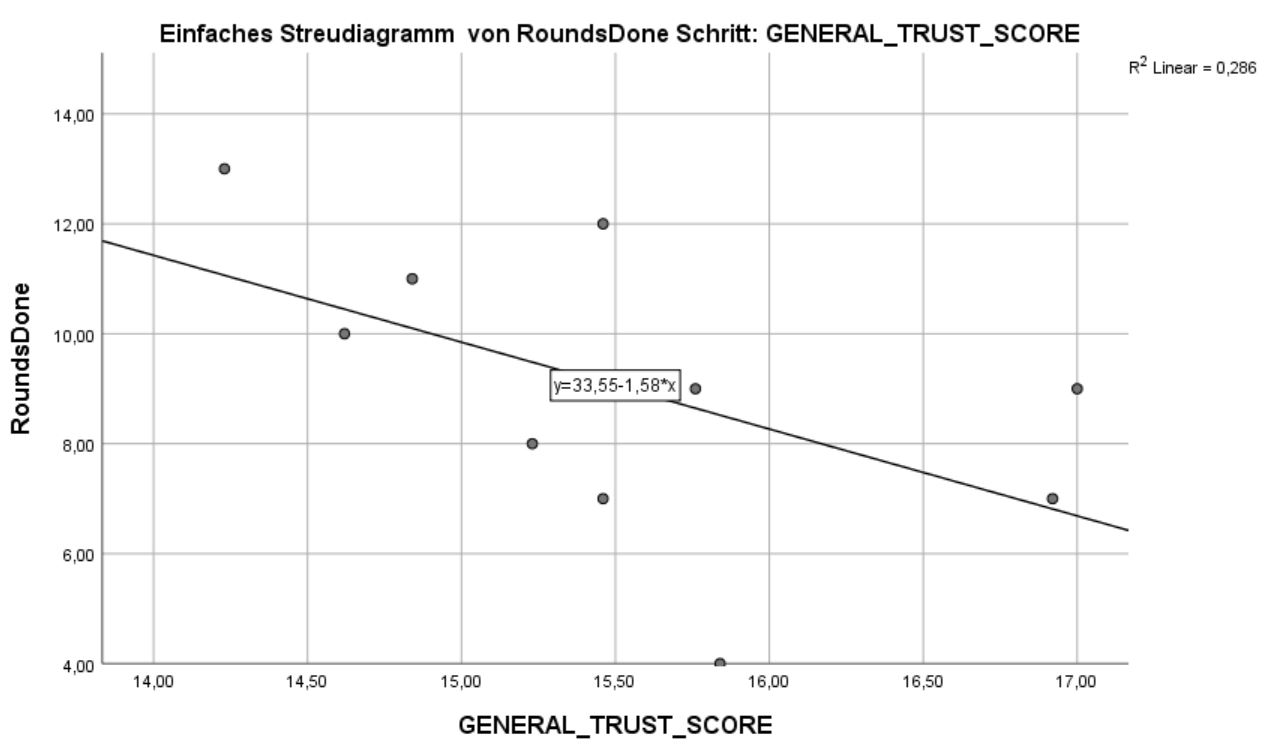
\includegraphics[scale=0.6]{Abbildungen/Post_QuestionnaireStatistiks/h5_both_diagramm_korr}
			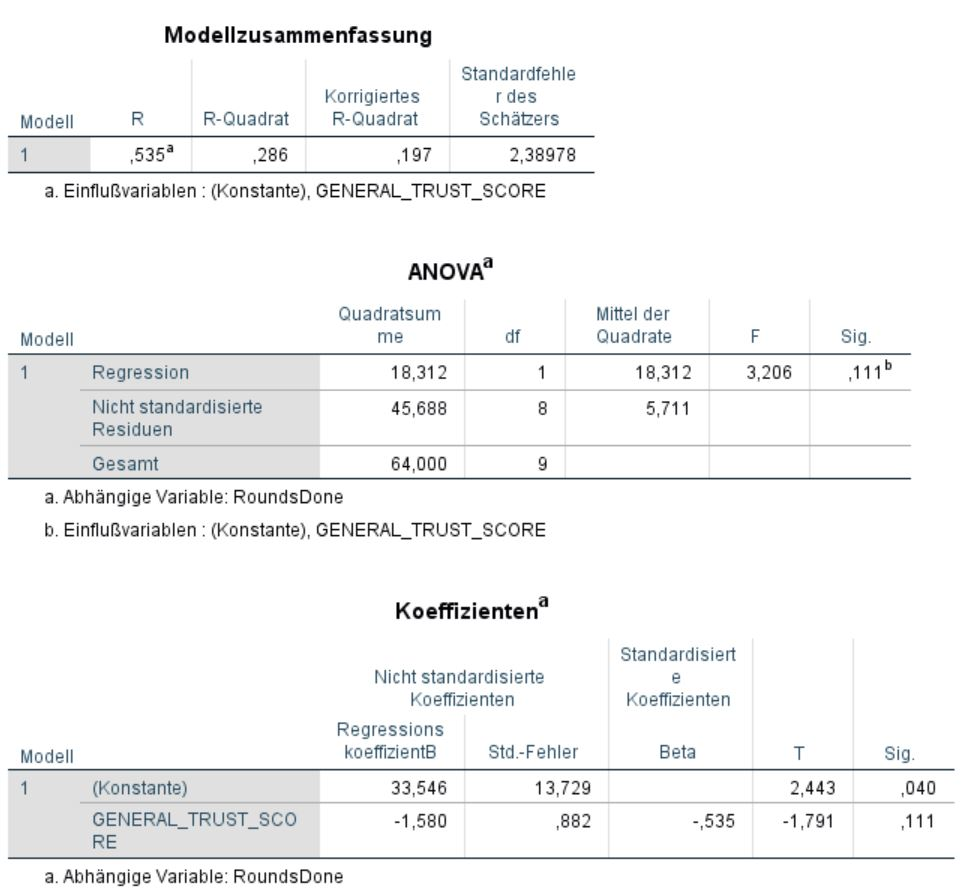
\includegraphics[scale=0.6]{Abbildungen/Post_QuestionnaireStatistiks/h5_both_regression}
			\caption{Regressionsergebnisse der Regressionen \ac{gt} und \ac{te} }
			\label{fig:h5_both}
		\end{footnotesize}
	\end{figure}	

\begin{figure}[H]
\centering
		\begin{footnotesize}
			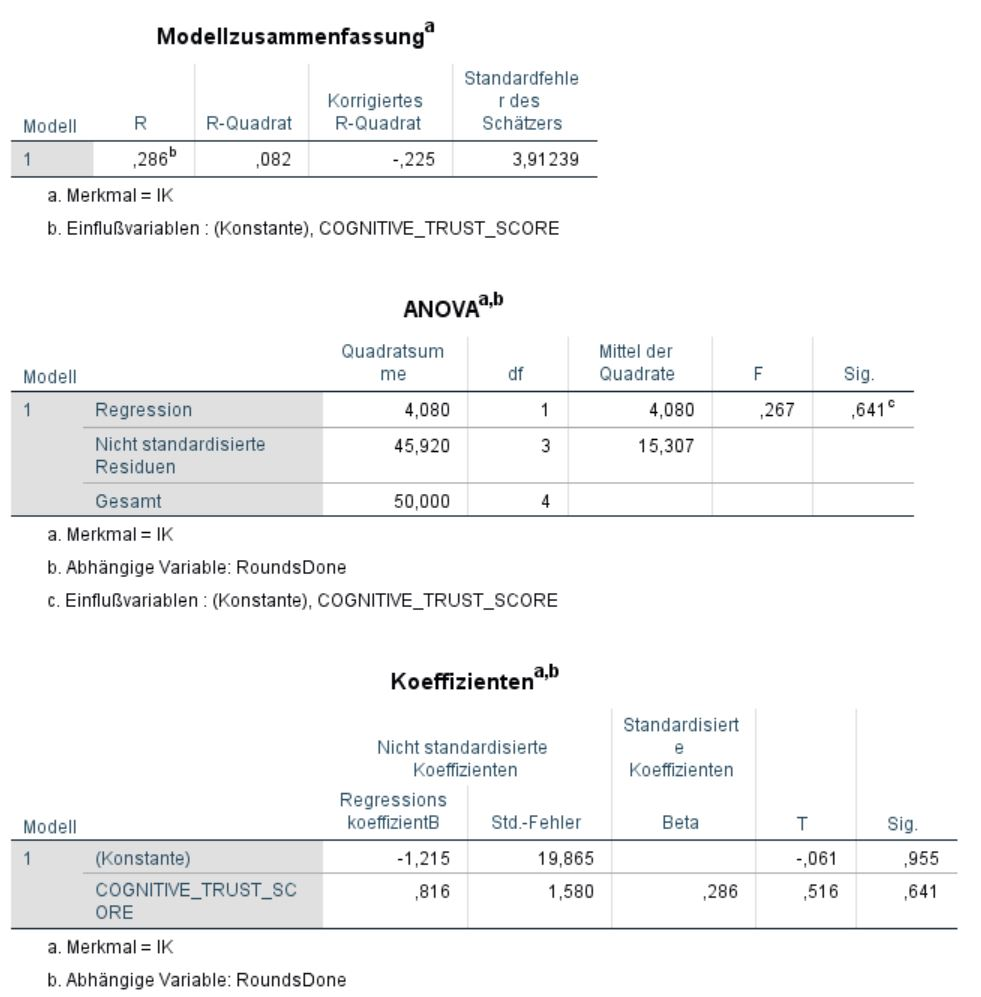
\includegraphics[scale=0.6]{Abbildungen/Post_QuestionnaireStatistiks/h3_regression_ik}
			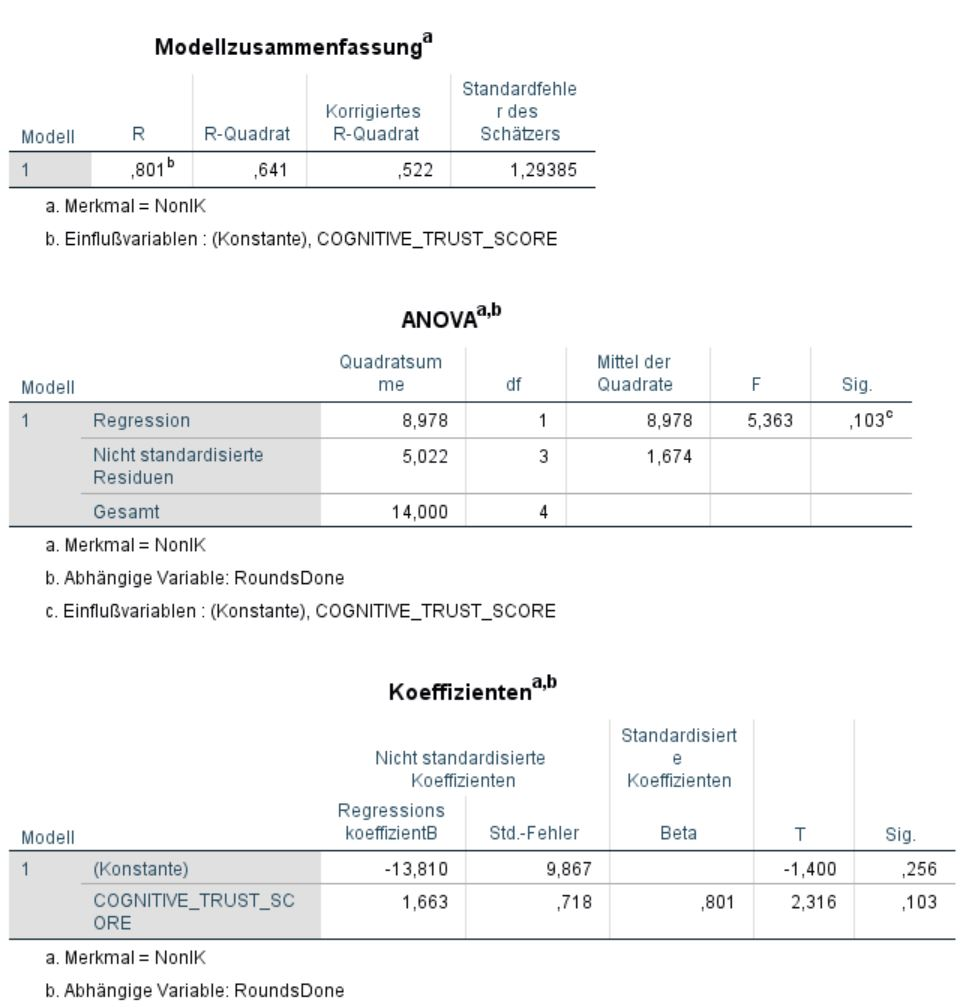
\includegraphics[scale=0.6]{Abbildungen/Post_QuestionnaireStatistiks/h3_regression_nik}
			\caption{Regressionsergebnisse der Regressionen \ac{gti} und \ac{tei} sowie \ac{gtn} und \ac{ten} }
			\label{fig:h5_regression}
		\end{footnotesize}
	\end{figure}	

\clearpage
\newpage
	\section{Demografieauswertung}
	\begin{figure}[H]
	\centering
		\begin{footnotesize}
			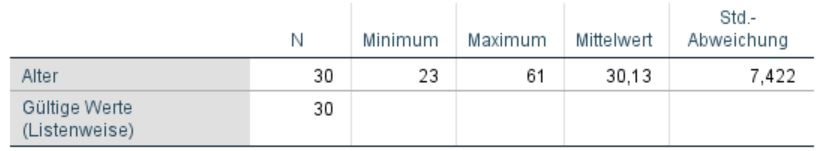
\includegraphics[scale=0.6]{Abbildungen/Pre_QuestionnaireStatistiks/teilnehmerStatistik}\\
			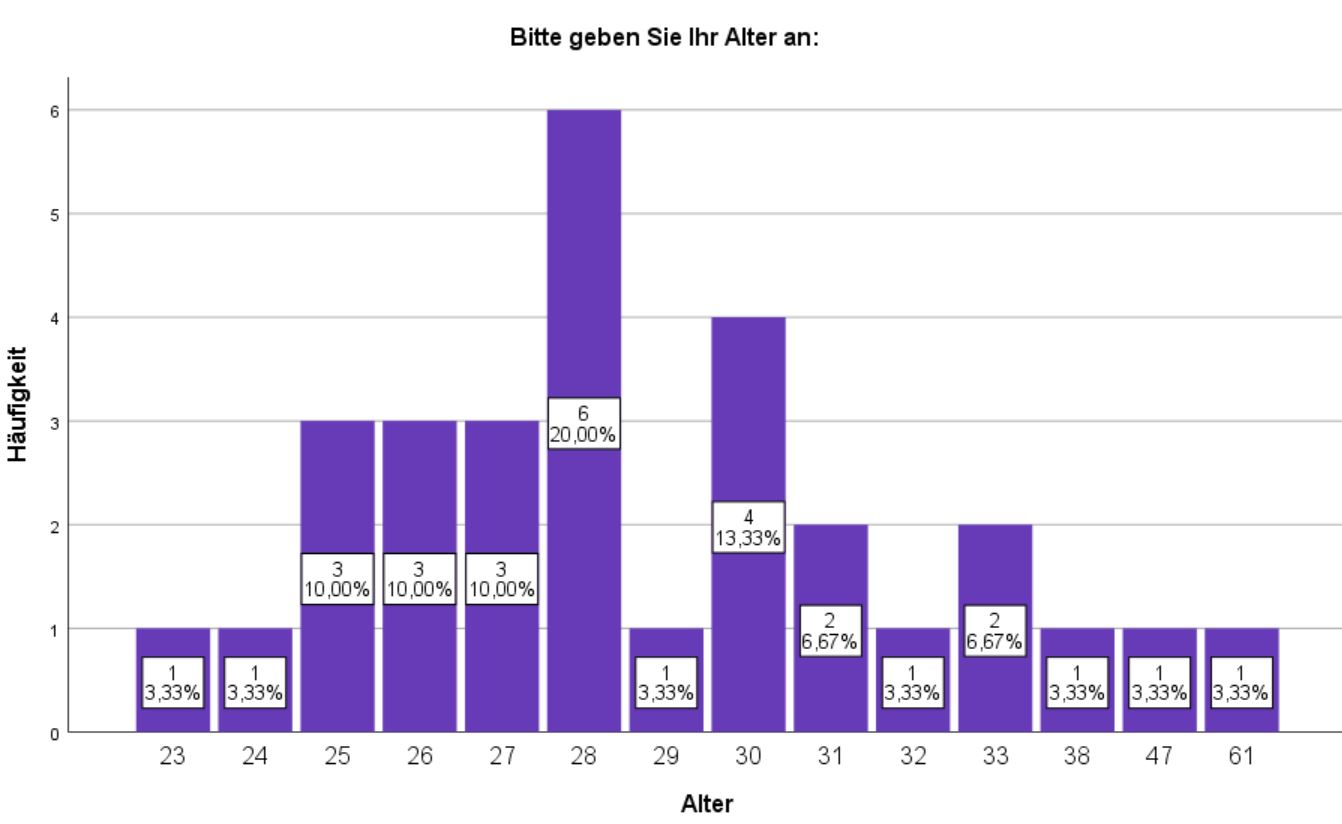
\includegraphics[scale=0.5]{Abbildungen/Demographie/alter}\\
			\caption{Alter der Teilnehmer}
			\label{fig:Teilnehmer}
		\end{footnotesize}
	\end{figure}	
	
	\begin{figure}[H]
	\centering
		\begin{footnotesize}
			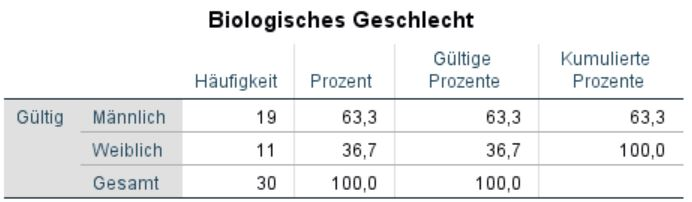
\includegraphics[scale=0.6]{Abbildungen/Pre_QuestionnaireStatistiks/teilnehmerGeschlecht}\\
			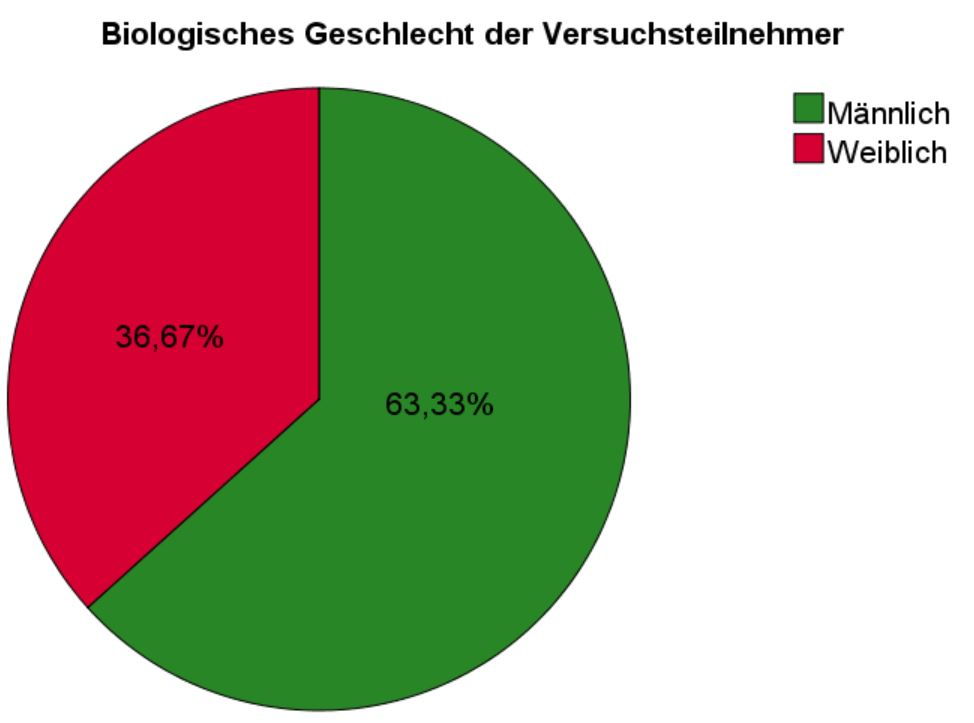
\includegraphics[scale=0.5]{Abbildungen/Demographie/teilnehmerGeschlecht}\\
			\caption{Biologisches Geschlecht der Teilnehmer}
			\label{fig:biologischesGeschlecht}
		\end{footnotesize}
	\end{figure}	
	
	\begin{figure}[H]
	\centering
		\begin{footnotesize}
			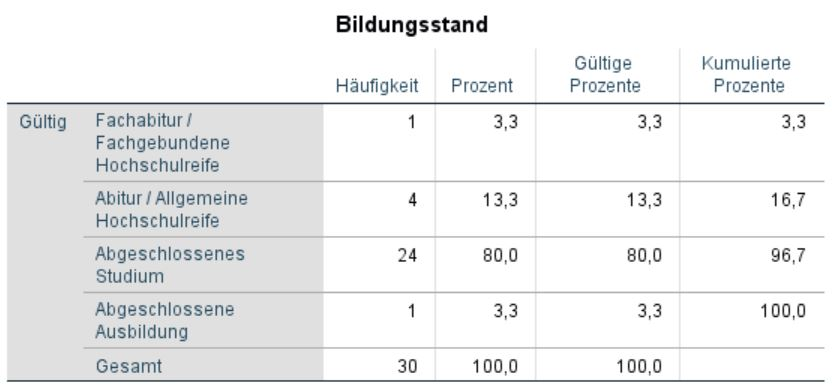
\includegraphics[scale=0.6]{Abbildungen/Pre_QuestionnaireStatistiks/teilnehmerBildungsstand}\\
			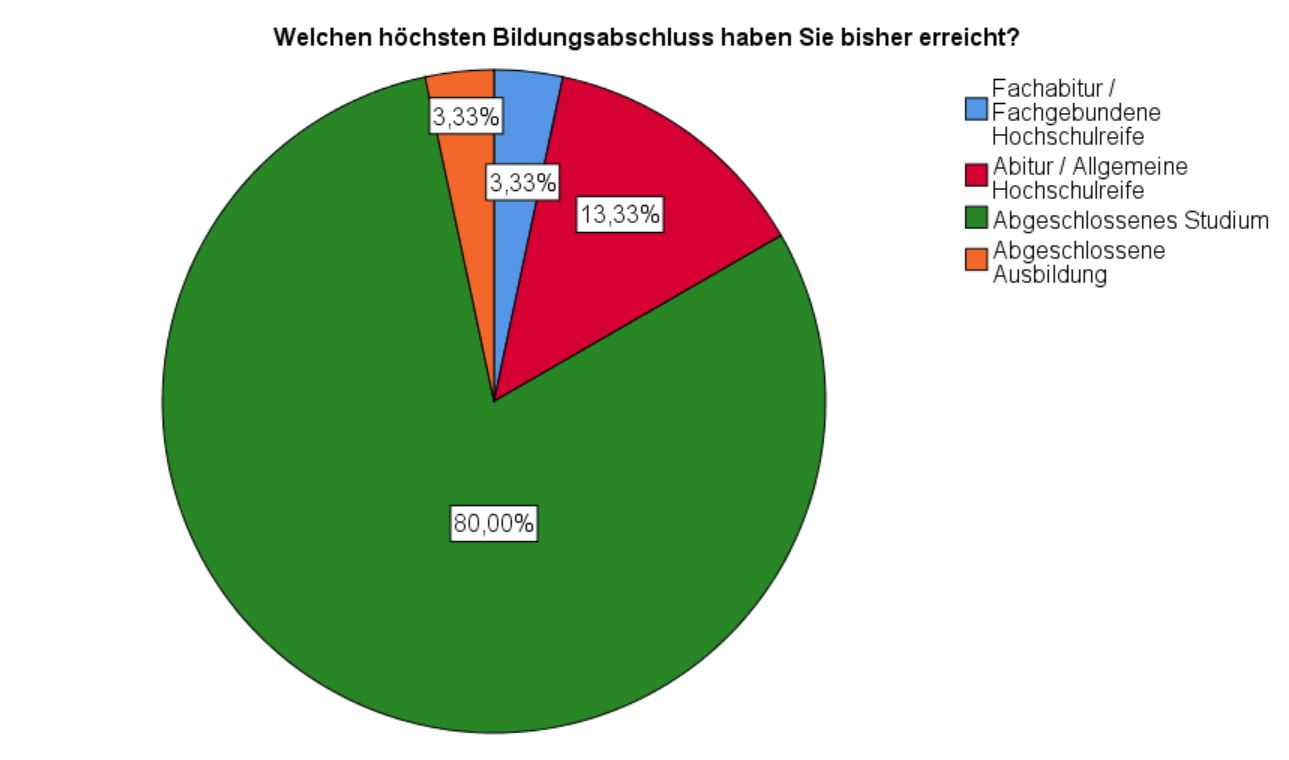
\includegraphics[scale=0.5]{Abbildungen/Demographie/teilnehmerBildungsstand}\\
			\caption{Bildungsstand der Teilnehmer}
			\label{fig:teilnehmerBildungsstand}
		\end{footnotesize}
	\end{figure}	
	
	\begin{figure}[H]
	\centering
		\begin{footnotesize}
			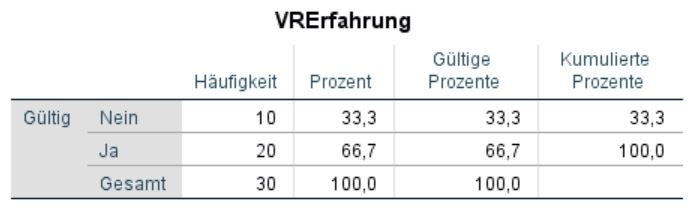
\includegraphics[scale=0.6]{Abbildungen/Pre_QuestionnaireStatistiks/teilnehmerVRErfahrung}\\
			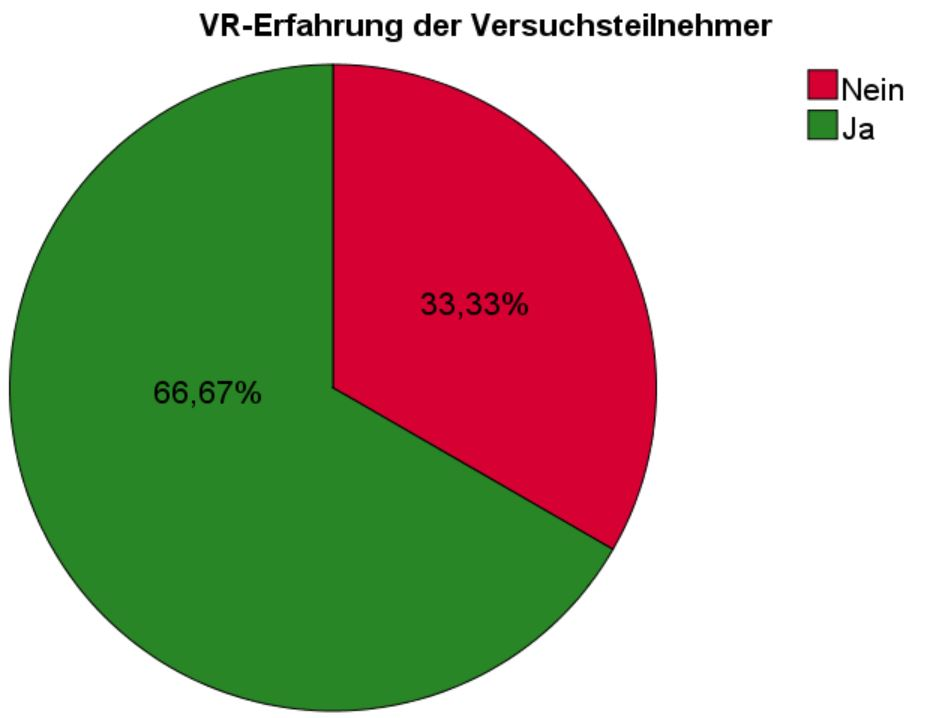
\includegraphics[scale=0.5]{Abbildungen/Demographie/teilnehmerVRErfahrung}\\
			\caption{VR-Erfahrung der Teilnehmer}
			\label{fig:teilnehmerVRErfahrung}
		\end{footnotesize}
	\end{figure}	
	
	\begin{figure}[H]
	[scale=0.6]
		\begin{footnotesize}
			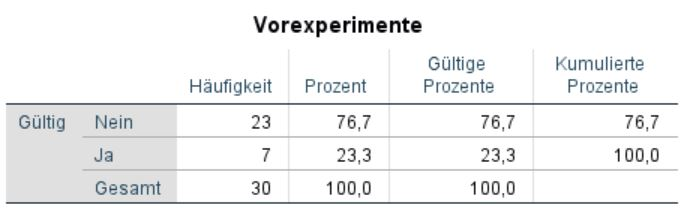
\includegraphics[scale=0.6]{Abbildungen/Pre_QuestionnaireStatistiks/teilnehmerVorexperimente}\\
			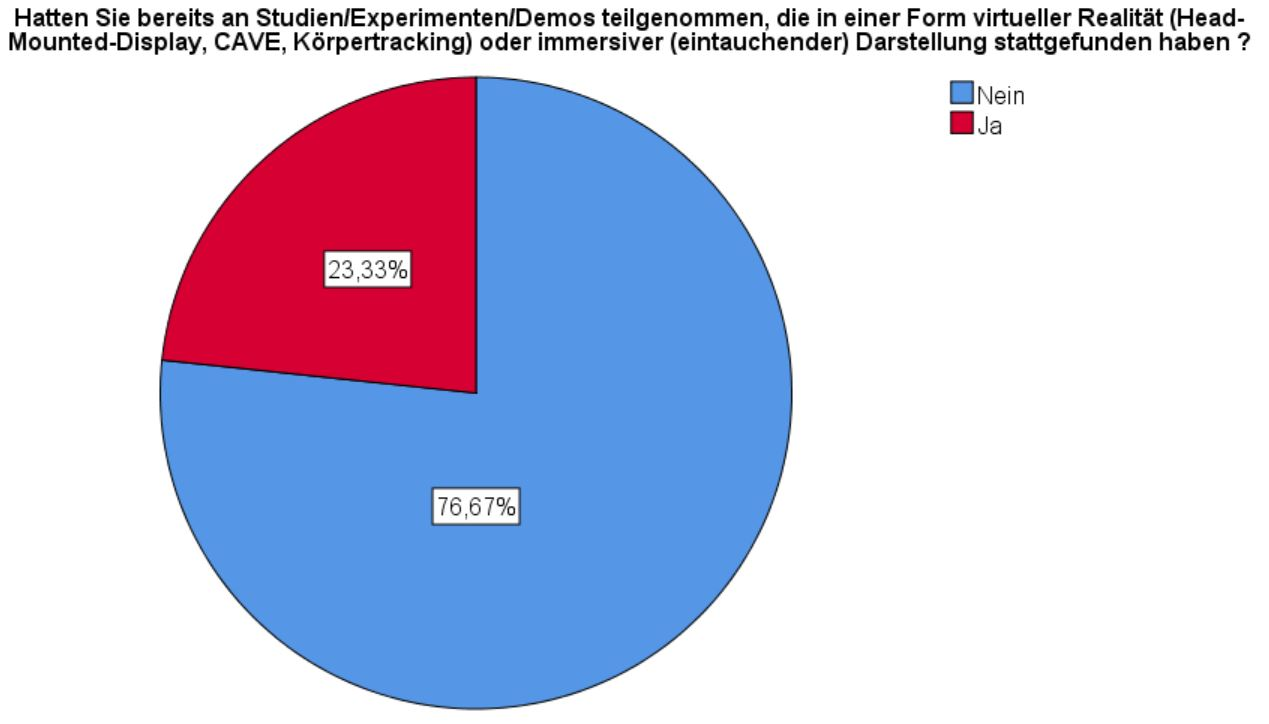
\includegraphics[scale=0.5]{Abbildungen/Demographie/teilnehmerVorexperimente}\\
			\caption{VR-Studien Vorerfahrungen}
			\label{fig:teilnehmerVorexperimente}
		\end{footnotesize}
	\end{figure}		
	
	\begin{figure}[H]
	\centering
		\begin{footnotesize}
			\includegraphics[scale=0.6]{Abbildungen/Pre_QuestionnaireStatistiks/teilnehmerPCAußmaß}\\
			\includegraphics[scale=0.5]{Abbildungen/Demographie/teilnehmerPCAußmaß}\\
			\caption{PC-Nutzung Außmaß sowie zugehörige Perzentile}
			\label{fig:teilnehmerPCAußmaß}
		\end{footnotesize}
	\end{figure}		
	
	\begin{figure}[H]
	\centering
		\begin{footnotesize}
			\includegraphics[scale=0.6]{Abbildungen/Pre_QuestionnaireStatistiks/teilnehmerVideospieleAußmaß}\\
			\includegraphics[scale=0.5]{Abbildungen/Demographie/teilnehmerVideospieleAußmaß}\\
			\caption{Videospieleaußmaß der Teilnehmer}
			\label{fig:teilnehmerVideospieleAußmaß}
		\end{footnotesize}
	\end{figure}		

	
	\section{Pre-Questionnaire}
	\label{Pre-Questionnaire}
	
	\begin{figure}[H]
	\centering
		\begin{footnotesize}
			\includegraphics[scale=0.6]{Abbildungen/Fragebogen/Pre-Questionnaire/PQ1}\\
		\end{footnotesize}
	\end{figure}	
	
	\begin{figure}[H]
	\centering
		\begin{footnotesize}
			\includegraphics[scale=0.6]{Abbildungen/Fragebogen/Pre-Questionnaire/PQ2}\\
		\end{footnotesize}
	\end{figure}	
	
	\begin{figure}[H]
	\centering
		\begin{footnotesize}
			\includegraphics[scale=0.6]{Abbildungen/Fragebogen/Pre-Questionnaire/PQ3}\\
		\end{footnotesize}
	\end{figure}	
	
	\begin{figure}[H]
	\centering
		\begin{footnotesize}
			\includegraphics[scale=0.6]{Abbildungen/Fragebogen/Pre-Questionnaire/PQ4}\\
		\end{footnotesize}
	\end{figure}	
	
	\begin{figure}[H]
	\centering
		\begin{footnotesize}
			\includegraphics[scale=0.6]{Abbildungen/Fragebogen/Pre-Questionnaire/PQ5}\\
		\end{footnotesize}
	\end{figure}	
	
	\begin{figure}[H]
	\centering
		\begin{footnotesize}
			\includegraphics[scale=0.6]{Abbildungen/Fragebogen/Pre-Questionnaire/PQ6}\\
		\end{footnotesize}
	\end{figure}	
	
\section{Post-Questionnaire - Konditionsabfrage}
\label{Post-Questionnaire - Konditionsabfrage}

	\begin{figure}[H]
	\centering
		\begin{footnotesize}
			\includegraphics[scale=0.6]{Abbildungen/Fragebogen/Post-Questionnaire/PQM1}
		\end{footnotesize}
	\end{figure}	

\newpage

\section{Post-Questionnaire - Generelles Vertrauen}
\label{Post-Questionnaire - Generelles Vertrauen}

	\begin{figure}[H]
	\centering
		\begin{footnotesize}
			\includegraphics[scale=0.6]{Abbildungen/Fragebogen/Post-Questionnaire/PQG1}
		\end{footnotesize}
	\end{figure}	
	
	\begin{figure}[H]
	\centering
		\begin{footnotesize}
			\includegraphics[scale=0.6]{Abbildungen/Fragebogen/Post-Questionnaire/PQG2}
		\end{footnotesize}
	\end{figure}	
	
	\begin{figure}[H]
	\centering
		\begin{footnotesize}
			\includegraphics[scale=0.6]{Abbildungen/Fragebogen/Post-Questionnaire/PQG3}
		\end{footnotesize}
	\end{figure}	
	
	\begin{figure}[H]
	\centering
		\begin{footnotesize}
			\includegraphics[scale=0.6]{Abbildungen/Fragebogen/Post-Questionnaire/PQG4}
		\end{footnotesize}
	\end{figure}	

\newpage
\section{Post-Questionnaire - Kognitives Vertrauen}	
\label{Post-Questionnaire - Kognitives Vertrauen}	

	\begin{figure}[H]
	\centering
		\begin{footnotesize}
			\includegraphics[scale=0.6]{Abbildungen/Fragebogen/Post-Questionnaire/PQC1}
		\end{footnotesize}
	\end{figure}	
	
	\begin{figure}[H]
	\centering
		\begin{footnotesize}
			\includegraphics[scale=0.6]{Abbildungen/Fragebogen/Post-Questionnaire/PQC2}
		\end{footnotesize}
	\end{figure}	

\newpage
\section{Post-Questionnaire - Teamkommunikation}	
\label{Post-Questionnaire - Teamkommunikation}	

\begin{figure}[H]
	\centering
		\begin{footnotesize}
			\includegraphics[scale=0.4]{Abbildungen/Fragebogen/Post-Questionnaire/PQKQ1}
		\end{footnotesize}
	\end{figure}	

\newpage
\section{Post-Questionnaire - Team-Effektivität}	
\label{Post-Questionnaire - Team-Effektivität}	

	\begin{figure}[H]
	\centering
		\begin{footnotesize}
			\includegraphics[scale=0.6]{Abbildungen/Fragebogen/Post-Questionnaire/PQTE1}
		\end{footnotesize}
	\end{figure}	

\newpage
\section{Post-Questionnaire - NASA-TLX}
\label{Post-Questionnaire - NASA-TLX}

	\begin{figure}[H]
	\centering
		\begin{footnotesize}
			\includegraphics[scale=0.6]{Abbildungen/Fragebogen/Post-Questionnaire/PQTLX1}
		\end{footnotesize}
	\end{figure}	
	
	\begin{figure}[H]
	\centering
		\begin{footnotesize}
			\includegraphics[scale=0.6]{Abbildungen/Fragebogen/Post-Questionnaire/PQTLX2}
		\end{footnotesize}
	\end{figure}	
	
	\begin{figure}[H]
	\centering
		\begin{footnotesize}
			\includegraphics[scale=0.6]{Abbildungen/Fragebogen/Post-Questionnaire/PQTLX3}
		\end{footnotesize}
	\end{figure}	
	
	\begin{figure}[H]
	\centering
		\begin{footnotesize}
			\includegraphics[scale=0.6]{Abbildungen/Fragebogen/Post-Questionnaire/PQTLX4}
		\end{footnotesize}
	\end{figure}	
	
	\begin{figure}[H]
	\centering
		\begin{footnotesize}
			\includegraphics[scale=0.6]{Abbildungen/Fragebogen/Post-Questionnaire/PQTLX5}
		\end{footnotesize}
	\end{figure}	
	
	\begin{figure}[H]
	\centering
		\begin{footnotesize}
			\includegraphics[scale=0.6]{Abbildungen/Fragebogen/Post-Questionnaire/PQTLX6}
		\end{footnotesize}
	\end{figure}	

\newpage
\section{Post-Questionnaire - IPQ}
\label{Post-Questionnaire - IPQ}

	\begin{figure}[H]
	\centering
		\begin{footnotesize}
			\includegraphics[scale=0.6]{Abbildungen/Fragebogen/Post-Questionnaire/PQP1}
		\end{footnotesize}
	\end{figure}	
	
	\begin{figure}[H]
	\centering
		\begin{footnotesize}
			\includegraphics[scale=0.6]{Abbildungen/Fragebogen/Post-Questionnaire/PQP2}
		\end{footnotesize}
	\end{figure}	
	
	\begin{figure}[H]
	\centering
		\begin{footnotesize}
			\includegraphics[scale=0.6]{Abbildungen/Fragebogen/Post-Questionnaire/PQP3}
		\end{footnotesize}
	\end{figure}	

\newpage
\section{Post-Questionnaire - Co-Presence}			
\label{Post-Questionnaire - Co-Presence}		

	\begin{figure}[H]
	\centering
		\begin{footnotesize}
			\includegraphics[scale=0.6]{Abbildungen/Fragebogen/Post-Questionnaire/PQCP1}
		\end{footnotesize}
	\end{figure}	
	
	\begin{figure}[H]
	\centering
		\begin{footnotesize}
			\includegraphics[scale=0.6]{Abbildungen/Fragebogen/Post-Questionnaire/PQCP2}
		\end{footnotesize}
	\end{figure}	
	
	\begin{figure}[H]
	\centering
		\begin{footnotesize}
			\includegraphics[scale=0.6]{Abbildungen/Fragebogen/Post-Questionnaire/PQCP3}
		\end{footnotesize}
	\end{figure}	
	
	\begin{figure}[H]
	\centering
		\begin{footnotesize}
			\includegraphics[scale=0.6]{Abbildungen/Fragebogen/Post-Questionnaire/PQCP4}
		\end{footnotesize}
	\end{figure}	
	
	\begin{figure}[H]
	\centering
		\begin{footnotesize}
			\includegraphics[scale=0.6]{Abbildungen/Fragebogen/Post-Questionnaire/PQCP5}
		\end{footnotesize}
	\end{figure}	
	
	\begin{figure}[H]
	\centering
		\begin{footnotesize}
			\includegraphics[scale=0.6]{Abbildungen/Fragebogen/Post-Questionnaire/PQCP6}
		\end{footnotesize}
	\end{figure}	

\section{Other}	
	
\begin{figure}[H]
		\begin{footnotesize}
			\includegraphics[scale=1]{Abbildungen/criteriaForVirtualTeams.JPG}
			\caption[Abbildung 1]{Kriterien für virtuelle Teams von \citep[p. 27]{schweitzer2010conceptualizing}}
			\label{criteriaForVirtualTeams}
		\end{footnotesize}
	\end{figure}	
	
	\begin{figure}[H]
	\centering
		\begin{footnotesize}
			\includegraphics[scale=0.6]{Abbildungen/CouchEtAl_1996_TrustScale}\\
			\caption[Abbildung 1]{Items of the Trust Inventory \citep[305-323]{couch1996assessment}}
			\label{Trust-Inventory}
		\end{footnotesize}
	\end{figure}
	

\end{document}
